%File: anonymous-submission-latex-2023.tex
\documentclass[letterpaper]{article} % DO NOT CHANGE THIS
% \usepackage[submission]{aaai23}  % DO NOT CHANGE THIS
\usepackage{aaai23}  % DO NOT CHANGE THIS
\usepackage{times}  % DO NOT CHANGE THIS
\usepackage{helvet}  % DO NOT CHANGE THIS
\usepackage{courier}  % DO NOT CHANGE THIS
\usepackage[hyphens]{url}  % DO NOT CHANGE THIS
\usepackage{graphicx} % DO NOT CHANGE THIS
\urlstyle{rm} % DO NOT CHANGE THIS
\def\UrlFont{\rm}  % DO NOT CHANGE THIS
\usepackage{natbib}  % DO NOT CHANGE THIS AND DO NOT ADD ANY OPTIONS TO IT
\usepackage{caption} % DO NOT CHANGE THIS AND DO NOT ADD ANY OPTIONS TO IT
\frenchspacing  % DO NOT CHANGE THIS
\setlength{\pdfpagewidth}{8.5in} % DO NOT CHANGE THIS
\setlength{\pdfpageheight}{11in} % DO NOT CHANGE THIS
%
% These are recommended to typeset algorithms but not required. See the subsubsection on algorithms. Remove them if you don't have algorithms in your paper.
\usepackage{algorithm}
\usepackage{algorithmic}

%
% These are are recommended to typeset listings but not required. See the subsubsection on listing. Remove this block if you don't have listings in your paper.
\usepackage{newfloat}
\usepackage{listings}
\DeclareCaptionStyle{ruled}{labelfont=normalfont,labelsep=colon,strut=off} % DO NOT CHANGE THIS
\lstset{%
	basicstyle={\footnotesize\ttfamily},% footnotesize acceptable for monospace
	numbers=left,numberstyle=\footnotesize,xleftmargin=2em,% show line numbers, remove this entire line if you don't want the numbers.
	aboveskip=0pt,belowskip=0pt,%
	showstringspaces=false,tabsize=2,breaklines=true}
\floatstyle{ruled}
\newfloat{listing}{tb}{lst}{}
\floatname{listing}{Listing}
%
% Keep the \pdfinfo as shown here. There's no need
% for you to add the /Title and /Author tags.
\pdfinfo{
/TemplateVersion (2023.1)
}

% DISALLOWED PACKAGES
% \usepackage{authblk} -- This package is specifically forbidden
% \usepackage{balance} -- This package is specifically forbidden
% \usepackage{color (if used in text)
% \usepackage{CJK} -- This package is specifically forbidden
% \usepackage{float} -- This package is specifically forbidden
% \usepackage{flushend} -- This package is specifically forbidden
% \usepackage{fontenc} -- This package is specifically forbidden
% \usepackage{fullpage} -- This package is specifically forbidden
% \usepackage{geometry} -- This package is specifically forbidden
% \usepackage{grffile} -- This package is specifically forbidden
% \usepackage{hyperref} -- This package is specifically forbidden
% \usepackage{navigator} -- This package is specifically forbidden
% (or any other package that embeds links such as navigator or hyperref)
% \indentfirst} -- This package is specifically forbidden
% \layout} -- This package is specifically forbidden
% \multicol} -- This package is specifically forbidden
% \nameref} -- This package is specifically forbidden
% \usepackage{savetrees} -- This package is specifically forbidden
% \usepackage{setspace} -- This package is specifically forbidden
% \usepackage{stfloats} -- This package is specifically forbidden
% \usepackage{tabu} -- This package is specifically forbidden
% \usepackage{titlesec} -- This package is specifically forbidden
% \usepackage{tocbibind} -- This package is specifically forbidden
% \usepackage{ulem} -- This package is specifically forbidden
% \usepackage{wrapfig} -- This package is specifically forbidden
% DISALLOWED COMMANDS
% \nocopyright -- Your paper will not be published if you use this command
% \addtolength -- This command may not be used
% \balance -- This command may not be used
% \baselinestretch -- Your paper will not be published if you use this command
% \clearpage -- No page breaks of any kind may be used for the final version of your paper
% \columnsep -- This command may not be used
% \newpage -- No page breaks of any kind may be used for the final version of your paper
% \pagebreak -- No page breaks of any kind may be used for the final version of your paperr
% \pagestyle -- This command may not be used
% \tiny -- This is not an acceptable font size.
% \vspace{- -- No negative value may be used in proximity of a caption, figure, table, section, subsection, subsubsection, or reference
% \vskip{- -- No negative value may be used to alter spacing above or below a caption, figure, table, section, subsection, subsubsection, or reference

\setcounter{secnumdepth}{2} %May be changed to 1 or 2 if section numbers are desired.

% The file aaai23.sty is the style file for AAAI Press
% proceedings, working notes, and technical reports.
%

% Title

% Your title must be in mixed case, not sentence case.
% That means all verbs (including short verbs like be, is, using,and go),
% nouns, adverbs, adjectives should be capitalized, including both words in hyphenated terms, while
% articles, conjunctions, and prepositions are lower case unless they
% directly follow a colon or long dash
% \title{Planning with Belief using Justified Perspectives}
\title{Planning with Multi-Agent Belief Using Justified Perspectives}
\author{
    %Authors
    % All authors must be in the same font size and format.
    % Written by AAAI Press Staff\textsuperscript{\rm 1}\thanks{With help from the AAAI Publications Committee.}\\
    % AAAI Style Contributions by Pater Patel Schneider,
    % Sunil Issar,\\
    Guang Hu,
    Tim Miller,
    Nir Lipovetzky
}
\affiliations{
    %Afiliations
    % \textsuperscript{\rm 1}Association for the Advancement of Artificial Intelligence\\
    % If you have multiple authors and multiple affiliations
    % use superscripts in text and roman font to identify them.
    % For example,

    % Sunil Issar, \textsuperscript{\rm 2}
    % J. Scott Penberthy, \textsuperscript{\rm 3}
    % George Ferguson,\textsuperscript{\rm 4}
    % Hans Guesgen, \textsuperscript{\rm 5}.
    % Note that the comma should be placed BEFORE the superscript for optimum readability
    
    School of Computing and Information Systems\
    The University of Melbourne\\
    Parkville, VIC 3010, AUS\\
    % email address must be in roman text type, not monospace or sans serif
    ghu1@student.unimelb.edu.au, tmiller@unimelb.edu.au, nir.lipovetzky@unimelb.edu.au
%
% See more examples next
}

% %Example, Single Author, ->> remove \iffalse,\fi and place them surrounding AAAI title to use it
% \iffalse
% \title{My Publication Title --- Single Author}
% \author {
%     Author Name
% }
% \affiliations{
%     Affiliation\\
%     Affiliation Line 2\\
%     name@example.com
% }
% \fi

% \iffalse
% %Example, Multiple Authors, ->> remove \iffalse,\fi and place them surrounding AAAI title to use it
% \title{My Publication Title --- Multiple Authors}
% \author {
%     % Authors
%     First Author Name,\textsuperscript{\rm 1}
%     Second Author Name, \textsuperscript{\rm 2}
%     Third Author Name \textsuperscript{\rm 1}
% }
% \affiliations {
%     % Affiliations
%     \textsuperscript{\rm 1} Affiliation 1\\
%     \textsuperscript{\rm 2} Affiliation 2\\
%     firstAuthor@affiliation1.com, secondAuthor@affilation2.com, thirdAuthor@affiliation1.com
% }
% \fi


% REMOVE THIS: bibentry
% This is only needed to show inline citations in the guidelines document. You should not need it and can safely delete it.
\usepackage{bibentry}
% END REMOVE bibentry



\usepackage{amsthm}
\usepackage{amssymb}
\usepackage{multirow}
\usepackage{multicol}
\usepackage{booktabs}
\usepackage{amsmath}
\usepackage{verbatim}

% \newcommand{\showPro}{Proposition}
% \newtheoremstyle{propositionstyle}% name
%   {5pt}%      Space above
%   {5pt}%      Space below
%   {}%         Body font
%   {}%         Indent amount (empty = no indent, \parindent = para indent)
%   {\itshape\bfseries}% Thm head font
%   {:}%        Punctuation after thm head
%   {\newline}%     Space after thm head: " " = normal interword space;
%         %       \newline = linebreak
%   {}%         Thm head spec (can be left empty, meaning `normal')
% \theoremstyle{propositionstyle}
% \newtheorem{Proposition}{Proposition}[section]
\theoremstyle{definition}
% \newtheorem{proposition}{Proposition}[section]

% \theoremstyle{definition}
\newtheorem{definition}{Definition}[section]
% \theoremstyle{definition}
\newtheorem{example}{Example}[section]
% \theoremstyle{definition}
\newtheorem{theorem}{Theorem}[section]
%\theoremstyle{definition}
\newtheorem{lemma}{Lemma}[section]
\newtheorem{plan}{Plan}[section]

% \usepackage{multicolumn}
\usepackage{listings}

\newcommand{\dom}{\textrm{dom}}

\newcommand{\timestamp}{ts}
\newcommand{\seq}{\Vec{s}}
% \newcommand{\bool}{\mathbb{B}}
\newcommand{\bool}{\{true,false\}}
\newcommand{\sees}{\triangleright}
\newcommand{\f}{\mathit{f}}
\newcommand{\observation}{\mathit{O}}
\newcommand{\memorization}{\mathit{R}}
\newcommand{\seen}{\mathbb{S}}
\newcommand{\unseen}{\neg \mathbb{S}}
\newcommand{\notknown}{\neg \mathbb{K}}
\newcommand{\cc}{\mathit{c}}

\def\L{\mathcal{L}}
\def\T{T}
\def\unknown{\frac{1}{2}}
\def\NF{\mathcal{N}\hspace{-0.5mm}\mathcal{F}}


\usepackage[textsize=scriptsize,textwidth=1cm]{todonotes}
% \usepackage[disable]{todonotes}
\newcommand{\tm}[1]{\vspace{0.5em}\todo[author=Tim,inline,color=green]{#1}\vspace{0.5em}}
\newcommand{\nl}[1]{\vspace{0.5em}\todo[author=Nir,inline,color=blue!20!white]{#1}\vspace{0.5em}}
\newcommand{\gh}[1]{\vspace{0.5em}\todo[author=Guang,inline,color=red!30!white]{#1}\vspace{0.5em}}
\newcommand{\rw}[1]{\vspace{0.5em}\todo[author=Reviewer,inline,color=yellow!30!white]{#1}\vspace{0.5em}}



\usetikzlibrary{calc,fadings,decorations.pathreplacing,automata}

\begin{document}

\maketitle

\begin{abstract}
Epistemic planning plays an important role in multi-agent and human-agent interaction domains. 
Most existing works solve multi-agent epistemic planning problems by either pre-compiling them into classical planning problems; or, using explicit actions and their effects to encode Kripke-based semantics. 
A recent approach called \emph{Planning with Perspectives} (PWP) delegates epistemic reasoning in planning to external functions using F-STRIPS, keeping the search within the planning algorithm and lazily evaluating epistemic formulae.
Although PWP is expressive and efficient, it models S5 epistemic logic and does not support belief, including false belief. 
In this paper, we extend the PWP model to handle multi-agent belief by following the intuition that agents believe something they have seen until they see otherwise. We call this \emph{justified perspectives}. We formalise this notion of multi-agent belief based on the definition of knowledge in PWP. Using experiments on existing epistemic and doxastic planning benchmarks, we show that our belief planner can solve benchmarks more efficiently than the state-of-the-art baseline, and can model some problems that are infeasible to model using propositional-based approaches.
\end{abstract}

% \tm{Just noting the title. In the Slack, you proposed `planning with belief using justified perspectives', which I think captures the work better}
% \gh{Sure. But what should the acronyms be? PBJP or PWBUJP, or PWBJP?}
\section{Introduction and Motivation}
\label{sec:intro}
In epistemic planning problems, agents need to reason about the ontic world and the epistemic world. 
There is extensive research on epistemic logic reasoning and epistemic planning, each with its own strengths and limitations. 
%The \emph{Dynamic Epistemic Logic} (DEL) ~\cite{DBLP:journals/jancl/BolanderA11,DBLP:conf/ecsi/Bolander14} based approach uses an event model to update an agent's belief through observations over actions.
%This approach uses different actions to update the ontic state, the epistemic state, and the agent's observability.
%There are two main drawbacks with DEL: 1)
%it has to explicitly model the high-order observability between agents; 
%2) it requires the modeller to understand the domain and the effects of each action with respect to the ontic an epistemic worlds.
Most epistemic planning approaches either explicitly maintain all epistemic relations, such as Kripke frames \cite{DBLP:conf/aips/KominisG15,DBLP:journals/jancl/BolanderA11,DBLP:conf/ecsi/Bolander14}, or require an expensive pre-compilation step to convert an epistemic planning problem into a classical planning problem~\cite{DBLP:journals/ai/MuiseBFMMPS22}, which grows exponentially w.r.t. the depth of the epistemic formula used.

Recently, \citet{Hu2022-ul} proposed a lazy-evaluation approach to epistemic planning called Planning with Perspectives (PWP).
They use Functional STRIPS (F-STRIPS) \cite{geffner2000functional} to separate epistemic reasoning from planning by modelling an agent's perspective using external functions, which can be customised for particular domains. 
The agent perspective function defines which variables each agent `sees' in each state, and from this, a multi-agent epistemic logic is built using the `what you get is what you see' paradigm~\cite{DBLP:conf/atal/GasquetGS14,DBLP:conf/ecsi/Bolander14,DBLP:conf/ecai/CooperHMMR16,DBLP:conf/lori/HerzigLM15}.
By doing so, epistemic reasoning can be performed without generating and reasoning over all epistemic relations. 
They show that they can handle more expressive problems than standard PDDL-based epistemic planners, and avoid the costly pre-compilation \cite{DBLP:conf/aaai/MuiseBFMMPS15,DBLP:journals/ai/MuiseBFMMPS22} and maintenance of Kripke models \cite{DBLP:journals/corr/Bolander17,DBLP:conf/aips/KominisG15,DBLP:conf/aips/LeFSP18,DBLP:conf/aips/FabianoBDP20,DBLP:journals/corr/abs-1909-13778/Causal_Belief_Decomposition_for_Planning_with_Sensing}.
In addition, their agent's perspective model only depends on the state variables valuation, so can be applied to model-free planners as long as they expose their current state, such as when planning with simulators~\cite{DBLP:conf/ijcai/FrancesRLG17}.

The weakness of PWP is that it can plan only with knowledge, but not belief.
By following \citeauthor{Fagin:2003:RK:995831}'s \shortcite{Fagin:2003:RK:995831} interpretation of the difference between knowledge and belief, in knowledge logic such as S5, $K_i \varphi \rightarrow \varphi$ is an axiom, while in belief logics such as KD45$_n$, it is not. Thus, approaches such as PWP cannot model problems in which agents can have incorrect beliefs.

In this paper, we extend the PWP approach to model \emph{justified belief}. We call this Planning with Multi-agent Belief using Justified Perspectives.
The intuition is that when people reason about something they cannot see, they generate \emph{justified} belief by retrieving information from their `memory' that supports that belief~\cite{goldman1979justified}. 
In our model, this information comes from the states they have observed in the past. 
So, an agent believes something if they saw it in the past, and has no evidence to suggest it no longer holds. 
This includes nested beliefs about other agents' beliefs.
We illustrate this idea with a classical false-belief example. 
\begin{figure*}[t!]
    \centering
    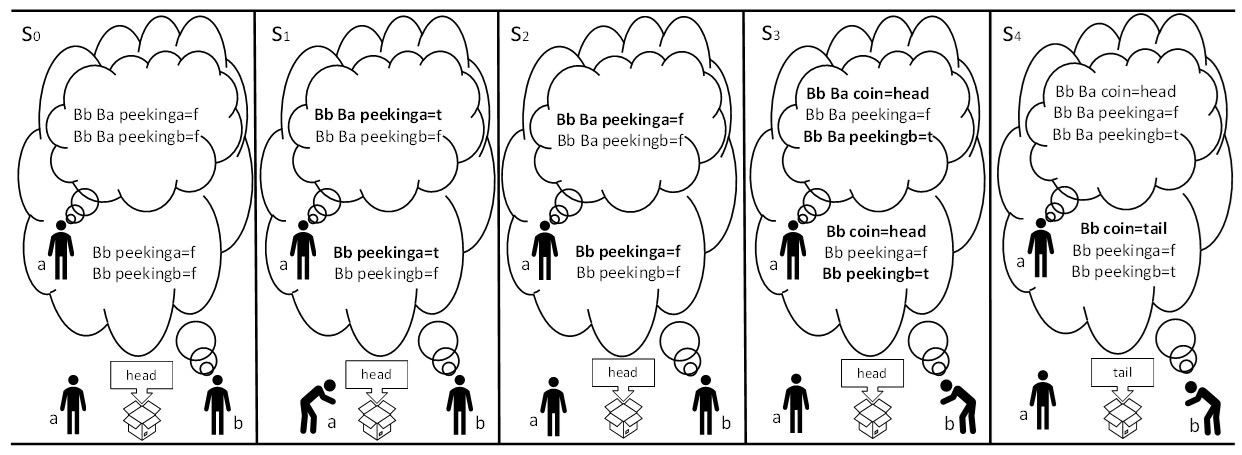
\includegraphics[width=0.9\textwidth]{Figures/plan_2_final.jpg}
    \caption{Plan~\ref{plan2} with agent $b$'s justified beliefs. Bold text indicates the belief that has changed.}
    \label{fig:plan_2_final}
\end{figure*}

\begin{example}
\label{example:coin}
There are two agents, $a$ and $b$, and there is a coin $c \in \{head,\ tail\}$ inside a box. 
The coin can only be seen by the agents when they are peeking into the box.
The agents can see each other all the time, which means they see whether others are peeking into the box. 
The actions that agents can take are ``\emph{peek}'' and ``\emph{return}'', while the coin can ``\emph{flip}'' itself at any point in time. The action and outcome of the flip is only visible to the agents who are peeking into the box.
Initially, both agent $a$ and $b$ are not peeking, and the coin is $head$.
The task is to generate a false belief such that: 
\begin{enumerate}
    \item the coin is $tail$;
    \item agent $b$ believes that the coin is $tail$; 
    \item agent $a$ believes that the coin is $head$; and 
    \item agent $b$ believes that agent $a$ believes that the coin is $head$.
\end{enumerate}
% 1. the coin is $tail$; 
% 2. agent $b$ believes the coin is $tail$; 
% 3. agent $a$ believes the coin is $head$; and 
% 4. agent $b$ believes that agent $a$ believes the coin is $head$.

\end{example}

% \begin{figure*}[h]
%     \centering
%     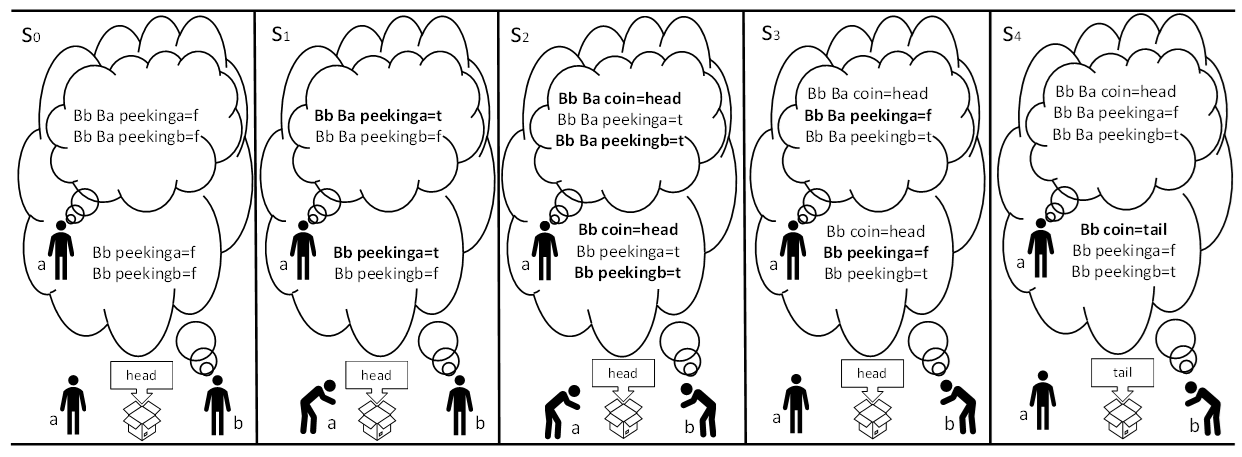
\includegraphics[width=0.9\textwidth]{Figures/plan_1_final.png}
%     \caption{Plan~\ref{plan1} with agent $b$'s justified beliefs. Bold text indicates belief that has changed.}
%     \label{fig:plan_1_final}
% \end{figure*}


% \begin{figure}
%     \centering
%     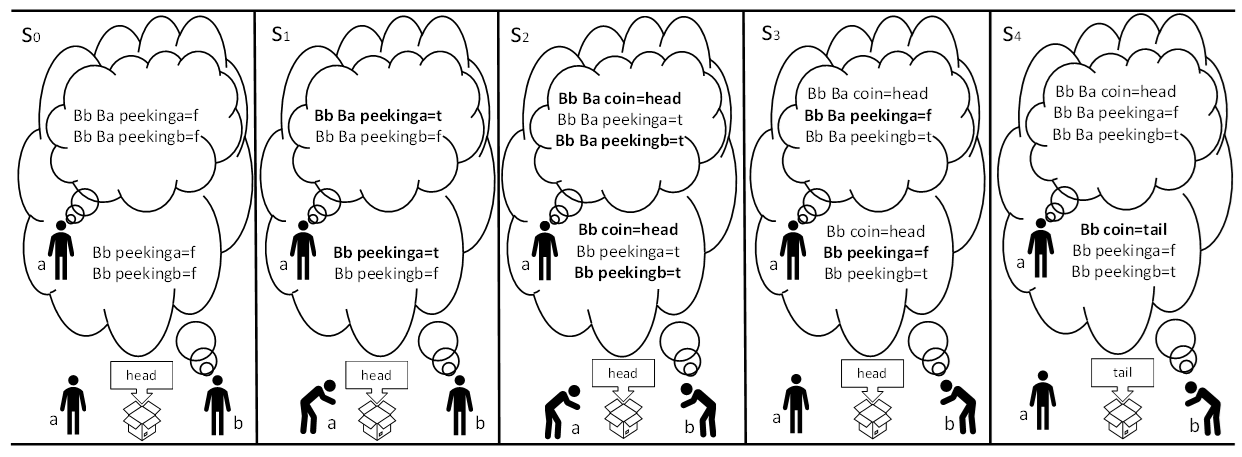
\includegraphics[width=0.95\columnwidth]{Figures/plan_1_final.png}
%     \caption{ Plan~\ref{plan1} to solve Example~\ref{example:coin}}
%     \label{fig:coin_plan_A}
% \end{figure}

% \tm{If you need to save space, I suggest dropping Plan 1.1 and just having Plan 1.2, which illustrates both of the main issues. If you have the space, keep both because the incremental building from 1.1 to 1.2 is nice}
% \gh{I am keeping a simplified version of plan 1.1}

A valid plan would be:
\begin{plan}
\label{plan1}
\emph{peek(a)}, \emph{peek(b)}, \emph{return(a)}, \emph{flip}
\end{plan}
It is intuitive that $B_b B_a coin=head$ holds, because agent $b$ saw agent $a$ peeked into the box after the action $\emph{peek(b)}$ and agent $a$ was not peeking into the box while $coin$ flipped.


\begin{comment}
A valid plan would be:
\begin{plan}
\label{plan1}
\emph{peek(a)}, \emph{peek(b)}, \emph{return(a)}, \emph{flip}
\end{plan}


As shown in Figure~\ref{fig:plan_1_final}, each criteria is reasoned as follows: 
\begin{enumerate}
    \item the coin becomes $tail$ in $s_4$; 
    \item agent $b$ believes (actually knows!) the coin is $tail$ as $b$ is peeking into the box in $s_4$; 
    \item agent $a$ believes coin is $head$ because the last state $a$ peeked into box is $s_2$ and the coin was $head$ in $s_2$, and has no evidence to disregard this;
    \item agent $b$ believes agent $a$ believes coin is $head$ because the last state $b$ saw $a$ peeking into the box is $s_2$ and the coin was $head$ in $s_2$. 
\end{enumerate}

Item 2 and 4 are worth discussing. 
For item 2, in state $s_4$, agent $a$ does not observe what is inside the box (the value of the coin).
Agent $a$ rather recalls the last time it saw the value of the $coin$ is $s_2$, and $a$ should ``remember'' the $coin$ is $head$.
For item 4, in  state $s_4$, agent $b$ observes that agent $a$ is not peeking into the box.
So, agent $b$ recalls that the last time $b$ saw $a$ see the value of the $coin$ was $s_2$ ($S_a coin$). 
Although it might be intuitive to use the value of the $coin$ from state $s_2$ to form the justified believe $B_b\ B_a coin=head$, the value we use should come from what agent $b$ believes the value was when agent $a$ peeked. 
It might look equivalent when analysing Plan~\ref{plan1}, but the former may lead the agent to hold no belief or a false-belief of the value compared to the actual value.
\end{comment}
% 1. the coin becomes $tail$ in $s_4$; 
% 2. agent $b$ believes (actually knows!) coin is $tail$ as $b$ is peeking into the box in $s_4$; 
% 3. agent $a$ believes coin is $head$ because the last state $a$ peeked into box is $s_2$ and coin was $head$ in $s_2$;
% 4. agent $b$ believes agent $a$ believes coin is $head$ because the last state $b$ saw $a$ peeking into the box is $s_2$ and the coin was $head$ in $s_2$. 

% \begin{figure}
%     \centering
%     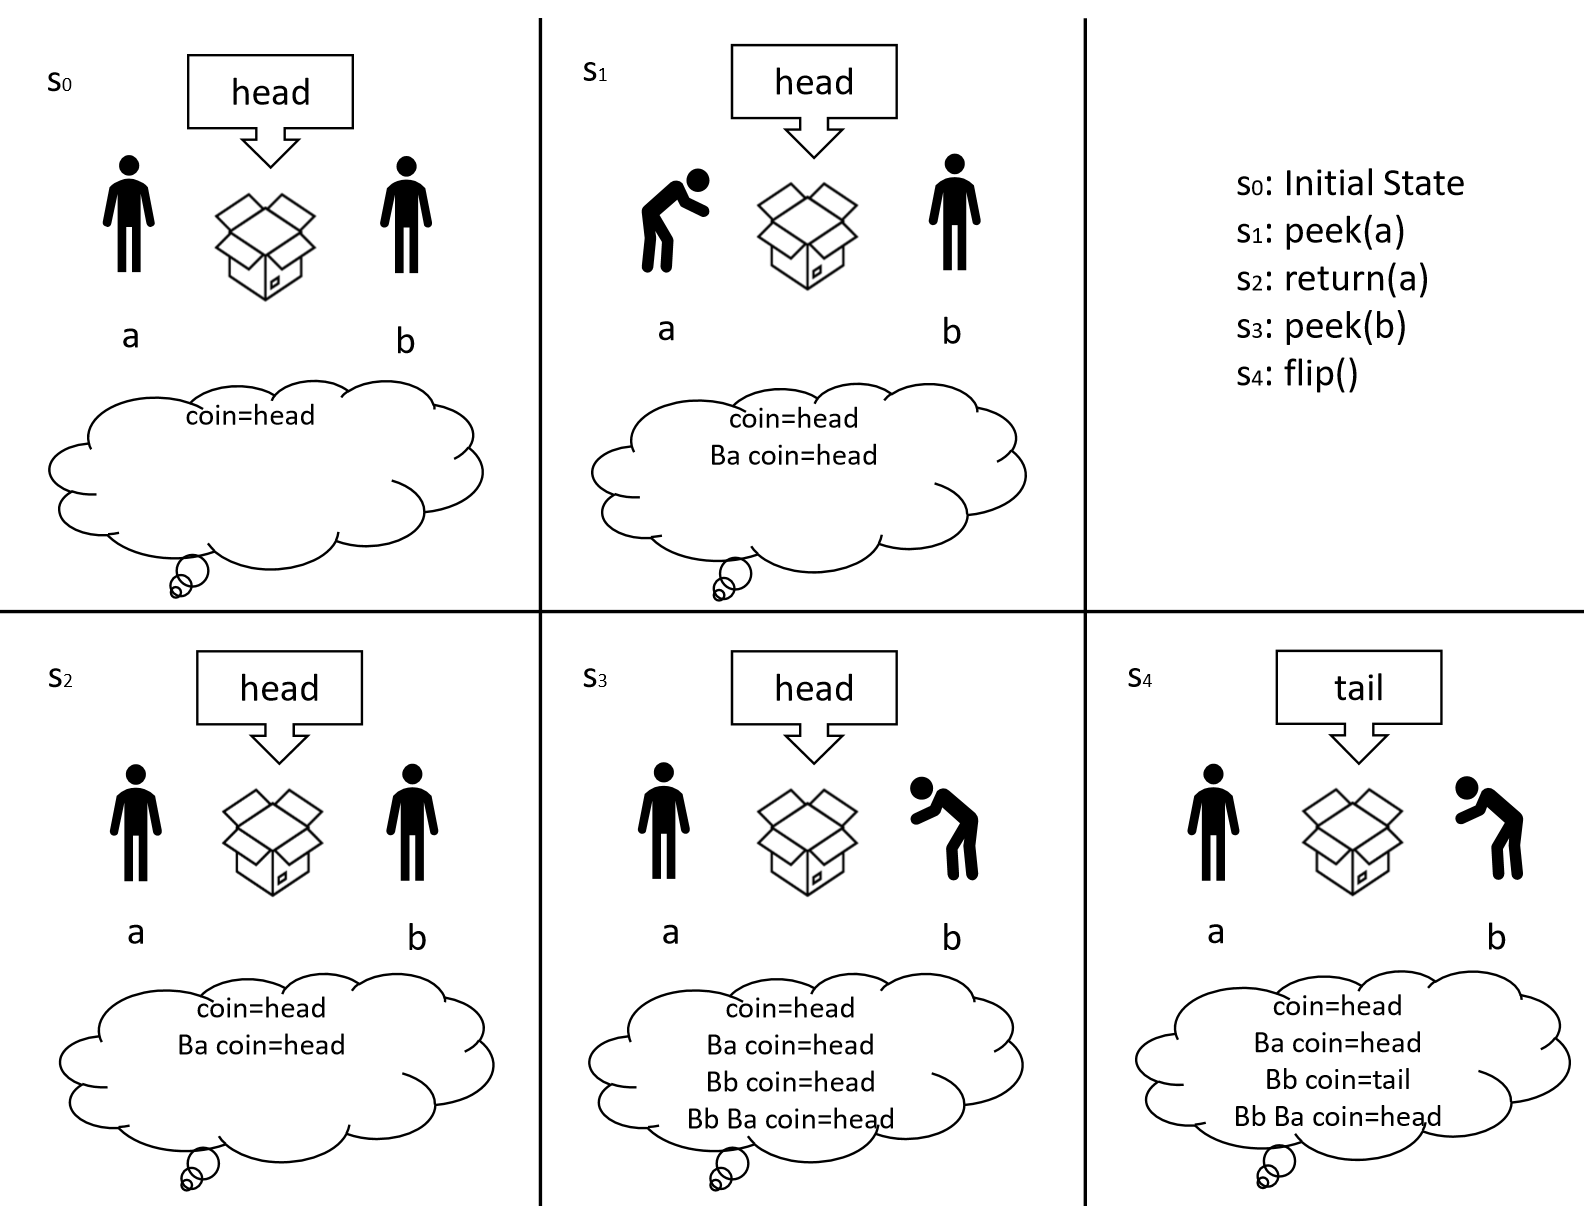
\includegraphics[width=0.9\columnwidth]{Figures/coin_plan2.png}
%     \caption{ Plan~\ref{plan2} to solve Example~\ref{example:coin}}
%     \label{fig:coin_plan_B}
% \end{figure}

A more challenging  plan to reason about, shown in Figure~\ref{fig:plan_2_final}), is:
\begin{plan}
\label{plan2}
\emph{peek(a)}, \emph{return(a)}, \emph{peek(b)}, \emph{flip}
\end{plan}



In this plan, agent $a$ and $b$ no longer peek into the box at the same time, which means, we do not have $K_b K_a coin=head$ in state $s_2$.
All criteria are met as in Plan~\ref{plan1}, except item 4.
For item 4, similarly, agent $b$ recalls that the last time it saw agent $a$ seeing the coin ($S_a coin$) was $s_1$.
However, agent $b$ holds no knowledge or belief on the value of the $coin$ from $s_1$, which means she cannot generate the justified belief in $s_1$.
Fortunately, agent $b$ gains belief of the coin from $s_3$.
So, agent $b$ still can justify its belief $B_b\ B_a coin=head$:
\begin{enumerate}
    \item $b$ recalls that the last time agent $a$ peeked inside of the box is $s_1$; and
    \item after $b$ saw $a$ peek, the next time $b$ saw the value of the $coin=head$ is at state $s_3$.
\end{enumerate}

In a model-free setting, reasoning about this is particularly challenging. 
Agents do not have access to the action model, so they cannot reason about what other agents have seen. 
Instead, they can only partially observe states and re-construct belief by observing states and who else observes each state.

This paper presents a model for KD45$_n$ belief over such plans, with the ability to solve model-free problems. Instead of keeping track of all possible beliefs, we instead use a lazy-evaluation approach that searches through previous states of the plan to re-construct what has been seen, and by who, to evaluate nested belief formulae. Our results show that we can efficiently solve existing benchmarks in epistemic and doxastic planning, even with a simple prototype planner.


% As shown in the Figure~\ref{fig:coin_plan_B}: 
% 1. the coin becomes $tail$ in $s_4$; 
% 2. agent $b$ believes (actually knows!) coin is $tail$ as $b$ is peeking into the box in $s_4$; 
% 3. agent $a$ believes coin is $head$ because the last state $a$ peeked into box is $s_2$ and coin was $head$ in $s_2$;
% 4. agent $b$ believes agent $a$ believes coin is $head$ because the last state $b$ saw $a$  peeking into the box is $s_2$ and the coin was $head$ in $s_2$. 



% The ability to reason about ones knowledge or belief beyond observation is another intelligent behaviour for epistemic agents. 
% Considering the following BBL example, which agents must be reason about two variables that they cannot observe at the same time.

% \tm{It is not clear to me that this BBL example gives much of a better idea than the coin task}

% \begin{example}
% \label{example:bbl}
% Agent $a$ and $b$ are two stationary cameras with certain vision range ($90^\circ$), and there is a target $x \in \{armed,\ unarmed\}$.
% Agent $b$ and target $x$ are located on the each side of agent $a$, which indicates that agent $a$ cannot see them both at the same moment.
% Agents do not know the location of each other nor target unless its within their sight. 
% The actions that agents can take is ``\emph{turn}'' and targets can take are ``\emph{pickup}'' and ``\emph{drop}''.
% Initially, agent $a$ faces west ($180^\circ$), agent $b$ faces west ($180^\circ$) and target $x$ is $armed$.
% The task is to generate a belief such that:
% 1. the target $x$ is $armed$;
% 2. agent $b$ knows the target $x$ is $armed$;
% 3. agent $a$ believes that agent $b$ knows the target $x$ is $armed$
% \end{example}
% % The two variables lies in separate boxes, and each agent is only able to look into one of the box at a time. In addition, agents know which box each other are looking at the moment.  

% % Example 1.0: Initially, let $x,y=1$ and $i \triangleright b_x, j \triangleright b_x$. Then, let us assume that agent $j$ looks away (e.g. turn to peek $b_y$), and the agent $i$ change the value of $x$ in box $b_x$ into $2$.
% To allow agent $a$ reason about agent $b$'s knowledge, agent $a$ needs to turn to be able to see agent $b$, $turn(-180^\circ)$, etc..
% Then, following the PWP model, agent $a$'s perspective contains agent $a$ and agent $b$ (target $x$ is not there).
% That is, agent $a$ can only reason about $b$'s perspective from $a$'s perspective of the world.
% Clearly, (3) does not hold as target $x$ is not in agent $a$'s perspective at all.
% It is obvious that some useful information, such as agent $a$ in the past knows target $x$ is $armed$, has lost during this process.

% Example 2.0: Can an agent gain the belief such as $x+y=2$?

% The tricky part is in this domain, agent is never able to see both variables at the same moment. So, that agent's belief about $x+y$ could be generated based on its belief over $x$ and $y$ separately rather than the belief over the relation $x+y$ as a whole.



\section{Background}

\subsection{Epistemic and Doxastic Logic}

\label{sec:background:epistemic_doxastic_logic}

% \subsubsection{Kripke Structure}
% Most of the works in epistemic logic using \emph{Kripke} models~\cite{Fagin:2003:RK:995831} as their theoretical base. 
% A Kripke model $M=\langle \mathcal{S}, \pi, \mathcal{K}_1,\dots,\mathcal{K}_n \rangle$ contains a set of worlds, interpretation function and accessibility relations between the worlds for each agent.
% The language that commonly used can be represented by:
% \[
%     \phi ::= p \mid \neg \phi \mid \phi \land \psi \mid K_i \phi \mid B_i \phi
% \]

% \tm{Guang, I would suggest that we don't need this level of detail. Things like Kripke semantics are briefly mentioned but not discussed. Just give an overview of logics for knowledge and belief, etc. The grammar for knowledge is given below in the PWP section}

% There are many interpretation on the beliefs~\cite{DBLP:journals/rsl/BjorndahlO20}.

The relation between knowledge and belief is not so clear.
Some authors state that knowledge is truthful belief~\cite{DBLP:journals/corr/DitmarschHHK15,DBLP:conf/kr/FriedmanH94,DBLP:conf/tark/FriedmanH94}, while others claim that knowledge is truthful \emph{justified} belief~\cite{DBLP:conf/nmr/Scherl22,DBLP:journals/rsl/Artemov08,DBLP:conf/atal/FanL17,DBLP:conf/kr/GrossiH14}.
\citet{DBLP:journals/rsl/BjorndahlO20} define the topology for knowledge and belief based on the different types of justification, while \citet{DBLP:conf/kr/GrossiH14} state that belief is generated, endorsed or justified by external arguments. 
However, there are no definitions of nested belief based on agents' previous observations.

% Some of the works state that $K_i \varphi$ if and only if $\varphi \land B_i \varphi$~\cite{DBLP:conf/kr/FriedmanH94,DBLP:conf/tark/FriedmanH94}, while some others extend this by adding the justification that $i$ is justified in believing $\varphi$~\cite{DBLP:conf/nmr/Scherl22,DBLP:journals/rsl/Artemov08,DBLP:conf/atal/FanL17}.

% \begin{comment}
Others use possible worlds to define both knowledge and belief~\cite{stalnaker2006logics,Fagin:2003:RK:995831}.
The idea in these logics is that the agents have a possibility relation $\mathcal{K}_i$ that models whether the agent $i$ can distinguish between two states.
Both the knowledge formula $K_i \varphi$ and belief formula $B_i \varphi$ are defined as that $\varphi$ holds in all the worlds that agent $i$ considers possible.
The difference is that possibility relation $\mathcal{K}_i$ in modelling knowledge needs to be \emph{reflective} and \emph{symmetric}\footnote{Reflective means for all $s\in \mathcal{S}$, $(s,s)$ must be in $\mathcal{K}$, while symmetric means if there is a possibility relation $(s,t)$ in $\mathcal{K}_i$, $(t,s)$ must also be in $\mathcal{K}_i$.}, while it is \emph{serial} in modelling beliefs.
Thus, such approaches have to maintain separate Kripke structures for handling knowledge and belief, and constraints between them must hold to ensure that certain properties hold; e.g.\ if an agent knows something then it believes it. In this paper, knowledge is based on what an agent currently `sees', while belief is based on what it currently sees and has  seen in the past.


The theoretical foundation for knowledge is the S5 axioms, while for belief are the KD45$_n$ axioms \cite{Fagin:2003:RK:995831}.
The difference between these two sets of axioms is that: 
S5 includes the axiom $K_i \varphi \rightarrow \varphi$ (Axiom T), which states that an agent's knowledge must be the truth (reflexivity); 
while KD45$_n$ does not have this axiom, so relations generated between possible worlds are derived from the agent's imperfect information of the world (could be false).
Axiom D, replacing T in KD45$_n$, captures $\neg K_i false$, which is preserved by the serial possibility relation.
% While the belief formula
% \end{comment}

% \gh{I changed the wording in the first sentence. The above paragraph is about how to use DEL approach modeling knowledge and beliefs, which mentioned a few times in introduction and background. Please feel free to remove it if you think it is not relevant :)  }
% \tm{Give a one sentence overview of how these authors deifne belief from knowledge.}
% \gh{Done}
% \tm{The above does not define belief though? How do they define belief from knowledge?}
% \gh{It is pretty hard to explain using one sentence. The idea is that the knowledge came from possibles worlds that is transitive, reflexive and \emph{symmetric}. while the belief needs to be \emph{serial}.}
% \gh{Done. Does this work?}
% \tm{Ok. I would say that `` define the knowledge first and derive belief from knowledge" is misleading. I thought the belief modal operator was defined in terms of knowledge; but this just extends the logic. So, I've removed this and just moved onto the next section. Is there anything else you think we should add here?}
% \gh{Maybe just changing the first sentence, and we can still keep this? unless you think this is not relevant:) We probably need it as in later section, we refer back to discuss there is no theoretical proof with possible worlds. }
\subsection{Epistemic Planning}

% Researchers in robotics face the problem of modeling robots' sensing.
% Many of them solving this problem use \emph{belief planning}.
% Belief planning is solving a search problem in belief space~\cite{DBLP:conf/aips/BonetG00}.
% They solve the problem by considering it as a partial-observable or non-deterministic planning problem, and using belief tracking, which require agents know how the model (action) works~\cite{DBLP:journals/corr/abs-1909-13778/Causal_Belief_Decomposition_for_Planning_with_Sensing,DBLP:conf/aaai/BonetG12a}.
% In addition, the objective of belief planning is to solve planning with incomplete information instead of generating and modeling agent's epistemic state.
% Thus, these approach does not allow agent to have belief or knowledge over others.

% \gh{The two paragraph below are added about epistemic planning}
Dynamic Epistemic Logic (DEL)  approaches use event models to track the agents' knowledge/belief over possible worlds. 
Most DEL approaches do not support false-belief because they are built on S5 logics. 
False-belief is challenging to model in DEL because it removes the `correct' possibility relation between worlds, which results in the agent's belief state becoming isolated~\cite{DBLP:journals/ai/BaralGPS22}.
% \citet{DBLP:journals/ai/BaralGPS22}'s work allows agents to 
So, in order to allow agents to recover from false-belief, it requires special sensing or announcing actions~\cite{DBLP:conf/aips/LeFSP18,DBLP:journals/ai/BaralGPS22,DBLP:journals/jolli/LiE22}.
In addition, it is costly to maintain all agents' possible worlds.
Although \citet{DBLP:conf/aips/KominisG15}'s work captures a fragment of DEL by tracking single agents' belief under the multi-agent setting and updating it by actions in order to achieve better computational performance, it still cannot handle false-belief.

As for the non-DEL-based approach, \citet{DBLP:journals/ai/MuiseBFMMPS22} define a proper epistemic knowledge base (PEKB) that contains all epistemic formulae as literals.
They convert an epistemic planning problem into a classical planning problem using the precondition and conditional effects in actions to update and revise the knowledge and belief literals following some modal axiom, such as those of KD45$_n$.
The advantage of their approach is that the model can be solved by any existing classical planner that supports conditional effects.
The limitations are: it cannot handle disjunctive belief; the depth of belief is bounded; and the number of literals grows exponentially on the depth of epistemic formulae, so the pre-compilation step has exponential time complexity.
\cite{DBLP:journals/ai/WanFL21} use a similar method that updates and revises belief knowledge base by implementing their own planner called MEPK, rather than converting to a classical planning problem.
By doing so, they lose the advantage of using an existing planner but gain  flexibility.
However, their approach still cannot handle false-belief.

% \tm{Above: can Wan's approach handle false belief? Make this clear}
% \gh{Cannot. Updated.}

% \tm{Add the PDKB stuff. I also suggest having one sentence on S5 planners, such as Huang's and Kominos, and just noting they solve for S5 not KD45}
% \gh{Done}




\subsection{Planning with Perspectives Approach}
\label{sec:background:pwp_appraoch}

\citet{Hu2022-ul} propose \emph{Planning with Perspectives} (PWP), which delegates epistemic reasoning to an external solver using F-STRIPS.

\paragraph{Signatures}
A PWP \emph{signature} is a tuple $\Sigma = (Agt, V, D_{v_1}, \ldots D_{v_n}, R)$, in which $Agt$ is a finite set of agent identifiers ($n$ of them), $V$ is a finite set of variables such that $Agt \subseteq V$ (agent identifiers can be used as variables), $D_{v_i}$ is a possibly infinite domain of constant symbols, one for each variable $v_i \in V$, and $R$ is a finite set of predicate symbols. Domains can be discrete or continuous, and the set of all values is defined as $D = \bigcup_{v\in V} D_v$.

\paragraph{Language}
The PWP language $\L(\Sigma)$ is defined by the grammar:
\[
    \varphi ::= r(\Vec{t}) \mid \neg \varphi \mid \varphi \land \varphi \mid S_i v \mid S_i \varphi \mid K_i \varphi,
\]
in which $r \in R$, vectors of terms $\Vec{t} \in V \cup D \cup Agt$, $i \in Agt$, and $v \in V$. A relation $r$ is a $k$-ary propositional relation; $S_i \varphi$ is a visibility formula that means agent~$i$ `sees' the truth value of formula $\varphi$, $S_i v$ is a visibility formula that means that agent~$i$ `sees' the value of the variable $v$, and $K_i \varphi$ is a knowledge formula. `Seeing' a formula is similar to `knowing whether` a formula is true or not \cite{DBLP:journals/rsl/FanWD15,DBLP:conf/aaai/MillerFMPS16}. `Seeing' should not be treated literally: an agent may `see' the value of a variable by hearing it through a communication channel, for example.

\paragraph{Model}
A model $M$ is defined $M=(Agt, V, D_{v_1}, \ldots, D_{v_k},\pi,\f_1,\dots,\f_n)$, in which $Agt$, $V$, $D_{v_i}$ are as in a signature.
A state $s: V \rightarrow D$ is a mapping from variables to values. 
A \emph{global state} is a total function (a complete assignment for all variables in $V$), while a \emph{local state} is a partial function (some variables may not be assigned). 
The expression $s(v)$  denotes the value of variable $v$ in state $s$. 
The set of all local and global states is denoted $\mathcal{S}$, while the set of all global states is $\mathcal{S}_G \subsetneq \mathcal{S}$. 
% We use $s(v_i)$ to represent the value of $v_i$ in $s$. 
% If variable $v_i$ is not in the domain of local state $s$, then $s(v_i)=null$. The set of all states (local and global) is denoted as $\mathcal{S}$, while the set of all global states is $\mathcal{S}_G \subsetneq \mathcal{S}$. 
The set of all models is denoted $\mathcal{M}$. 
$\pi$ is an interpretation function $\pi : \mathcal{S} \times R \rightarrow \{true,false\}$ that determines whether the atomic term $r(\Vec{t})$ is true in $s$. 
$r$ is undefined if any of its arguments $t_i$ is a variable $v\in V$ that is not assigned a value in a local state $s$, i.e. $v \not\in dom(s)$.


\paragraph{Perspective Function}
The key idea in the PWP model is the \emph{perspective function}.
A perspective function for agent $i$, $\f_i: \mathcal{S} \rightarrow \mathcal{S}$ is a function that takes a state and returns a subset of that state, which represents the part of that state that is visible to agent~$i$. 
The following properties must hold on a perspective function, $\f_i$ for all $i \in Agt$ and $s \in \mathcal{S}$:

% \vspace{2mm}
% \begin{tabular}{ll}
%  (1) & $\f_i(s) \subseteq s$ \\[1mm]
%  (2) & $\f_i(s) = \f_i(\f_i(s))$\\[1mm]
%  (3) & If $s \subseteq s'$, then $\f_i(s) \subseteq \f_i(s')$
% \end{tabular}
% \vspace{2mm}

\vspace{2mm}
\begin{tabular}{ll}
 (1) & $\observation_i(s) \subseteq s$ \\[1mm]
 (2) & $\observation_i(s) = \observation_i(\observation_i(s))$\\[1mm]
 (3) & If $s \subseteq s'$, then $\observation_i(s) \subseteq \observation_i(s')$
\end{tabular}
\vspace{2mm}



\citeauthor{Hu2022-ul} define general perspective functions, but note that perspective functions can be customised for domains. This provides a level of expressiveness not possible in declarative languages such as PDDL.


\paragraph{Complete Semantics}
\citet{Hu2022-ul} propose a sound and complete semantics for PWP\footnote{They call these semantics the `non-na\"ive' semantics, but we use the term `complete' in this paper as we do not have present a `na\"ive' semantics as \citet{Hu2022-ul} do.}.

\begin{definition}
\label{def:pwp:individual_semantics}

Given a model $M$ and state $s$, the truth of a PWP formula is defined as:

\vspace{2mm}
\noindent
\begin{tabular}{ll@{~~}l@{~~~}l}
 (a) & $M,s \vDash r(\vec{t})$ & iff & $\pi(s, r(\vec{t})) = true$\\[1mm]
 (b) & $M,s \vDash \phi \land \psi$  & iff & $M,s \vDash \phi$ and $M,s \vDash \psi$\\[1mm]
 (c) & $M,s \vDash \neg \varphi$     & iff & $M,s \not\vDash \varphi$\\[1mm]
 (d) & $M,s \vDash S_i v$            & iff & $v \in \dom(f_i(s))$\\[1mm]
 (e) & $M,s \vDash S_i \varphi$      & iff & 
     $\forall g \in \mathcal{S}_G$, $M,g[f_i(s)] \vDash \varphi$  or \\ 
   &  & & $\forall g \in \mathcal{S}_G$, $M,g[f_i(s)] \vDash \neg \varphi$ \\[1mm]
\end{tabular}
\vspace{2mm}
where: $\vec{t}$ is the terms in the relation $r$, and where $g[s]$ is defined as an override function, where $g[s](v) = s(v)$ if  $v \in \dom(s)$, and $g(v)$ otherwise.
So, the truth value of $S_i \varphi$ is such that $\varphi$ is true in every possible state based on the partial view of agent $i$, or false in every possible state based on the partial view of agent $i$.

From this, echoing \citet{DBLP:conf/ecai/CooperHMMR16}, the knowledge operation is defined as:
$K_i \varphi \leftrightarrow S_i \varphi \land \varphi$.
That is, agent $i$ knows $\varphi$ iff $\varphi$ is true and agent $i$ can see whether $\varphi$ is true.
\end{definition}

\paragraph{Ternary Semantics}
\citet{Hu2022-ul} show that the complete PWP semantics has exponential time complexity---in the $S_i \varphi$ definition, we must iterate over all global states $\mathcal{S}_G$. To counter this, they propose a polynomial time \emph{ternary} semantics \cite{levesque1998completeness}, which contains truth values 0 (false), 1 (true), and $\unknown$ (not known). They define a function $T$, which evaluates the value of the formula, defined as follows (omitting $M$ for readability):

\vspace{2mm}
\noindent
\begin{tabular}{@{}lllll}
 (a) & $T[s, r(\vec{t})]$ & =
         &  $1$ if $\pi(s_n, r(\vec{t})) = true$; \\
     & & &  $0$ if $\pi(s_n, r(\vec{t})) = false$; \\
     & & &  $\unknown$  otherwise\\[2mm]

 (b) & $ T[s, \phi \land \psi]$ & = & $\min(T[s_n,\phi]$, $ T[s_n,\psi]$)\\[2mm]
 (c) & $T[s,\neg \varphi]$ & = &  $1-T[s_n, \varphi]$\\[2mm]
%  (d) & \multicolumn{2}{l}{ $ T[s \vDash S_i v]=$}            \\ & = & $v \in \observation_i(s_n)$\\[2mm]

 (d) & $T[s, S_i v$] & = 
        & $\unknown$  if $ i \notin \dom(s_n)$ or $v \notin \dom(s_n)$;\\
     &&   & $0$ if  $v \notin \dom(\f_i(s_n))$;\\
     &&   & $1$ otherwise\\[2mm]
 (e) & $T[s,S_i \varphi]$ & = 
        & $\unknown$ if $T[s_n,\varphi]=\unknown$ or $i \notin \dom(s)$\\
      &&  & $ 0 $  if $ T[\f_i(s_n),\varphi]=\unknown$\\
      &&  & $ 1 $  otherwise
%  (f) & $T[s, K_i\varphi]$ & = & $T[s, \varphi \land S_i \varphi]$ \\[1mm] 
%  (f) & $T[s, B_i \varphi]$ & = & $ T[\f_i(s), \varphi]$  \\[1mm] 
\end{tabular}
\vspace{2mm}

They prove that this semantics is sound on all formulae, and is also complete for a fragment of the language known as $\NF$. 
This fragment $\NF$  captures formulae such as those that do not contain tautologies or contradictions. Given perspective functions for each agent, knowledge formulae in preconditions and effects are evaluated by an F-STRIPS external function that implements the ternary semantics. 
This approach is considerably more efficient that the PDKB baseline \citet{DBLP:journals/ai/MuiseBFMMPS22}, while offering more expressiveness.

% \subsubsection{Common Perspective}
% They define the common perspective of a group as a perspective fixed point when apply infinite level of nest as follows:

% \begin{definition}
% \label{def:fix_point}
%     Let $s$ be the given state and $G$ a group of agents, a perspective fixed point $\cc\f(G,s)=s'$ can be defined as:
%     \[
%         \cc\f(G,s')=\cc\f(G,\bigcap _{i \in G} \f_i(s'))
%     \]
% \end{definition}
% That is, using joint everyone's perspective of a given state as input, generate joint nested perspective for everyone until reached a fix point (could be empty).


% \subsubsection{Group Semantics}
% Similar as Individual semantics, their give their group semantics with three formats as well.
% For simplicity, we only show the definition of their Na\"ive Semantics as follows:

% \begin{definition}
% \label{def:pwp:group_semantics}
% Given a model $M$ and state $s$, their group semantics for seeing formulae can be defined as follows:

% \vspace{2mm}
% \begin{tabular}{llll}
% 	(g) & $ M,s \vDash ES_G\alpha$   & iff & for all $i\in G$, $ M,s \vDash S_i\alpha$\\[1mm]
% 	(h) & $ M,s \vDash DS_G v$       & iff & \(v \in dom(\bigcup_{i\in G}\f_i(s))\)\\[1mm]
% 	(i) & $ M,s \vDash DS_G \varphi$ & iff & $ M,s' \vDash \varphi$\\
% 	    &                            &     & or $ M,s' \vDash \neg\varphi$,\\
% 	    & & \multicolumn{2}{l}{where $s'=\bigcup_{i\in G}\f_i(s)$} \\[1mm]
% 	(j) & $ M,s \vDash CS_G v$       & iff & $v \in \dom(\cc\f(G,s))$\\[1mm]
% % 	(k) & $ M,s \vDash CS_G \varphi$ & iff & for all $g \in \mathcal{S}_G$, $ M,g[s']) \vDash \varphi$ \\
% % 	& & & or for all $g \in \mathcal{S}_G$, $ M,s' \vDash \neg\varphi$, where $s'= \cc\f(G,s)$.
% 	(k) & $ M,s \vDash CS_G \varphi$ & iff & $ M,s' \vDash \varphi$\\
% 	    &                            &     & or $ M,s' \vDash \neg\varphi$,\\
% 	    & & \multicolumn{2}{l}{where $s'= \cc\f(G,s)$} \\[1mm]
% \end{tabular}
% \vspace{2mm}
% \end{definition}

% Then, following the equivalency between knowledge and seeing, they can derived the semantics for group knowledge formulae.

% \begin{definition}
% \label{def:group_equiv}
% The equivalent relations between group seeing and group knowledge can be defined as:

% \vspace{2mm}
% \begin{tabular}{l}
%     $ EK_G \varphi \leftrightarrow \varphi \land ES_G \varphi \leftrightarrow \bigwedge i\in G K_i \varphi$\\[1mm]
%     $DK_G \varphi \leftrightarrow \varphi \land DS_G$\\[1mm]
%     $CK_G \varphi \leftrightarrow \varphi \land CS_G$\\[1mm]
% \end{tabular}
% \vspace{2mm}
% \end{definition}

% By following \cite{Fagin:2003:RK:995831}'s interpretation of difference between knowledge and belief, in the logic S5, $K_i \varphi \rightarrow \varphi$ is an axiom, while in belief logics that as KD45, $B_i \varphi \rightarrow \varphi$ is not an axiom, which implies that $B_i \varphi$ and $\neg \varphi$ can be both true simultaneously. 



\section{Justified Perspective Model}

In this section, we add a belief operator, $B_i$, to the PWP model \cite{Hu2022-ul}. This belief operator captures the intuition that we believe  something if we have  seen it before, and we have seen no contradicting evidence since. 
% \gh{maybe say something like: Although we give all necessary definitions, space limitations demand we do this succinctly. Or it is already a common knowledge among the researchers?}

\subsection{Language and Model}

%\begin{definition}[Signature]
%\label{def:signature}
%A \emph{signature} is a tuple $\Sigma = (Agt, V, D_{v_1}, \ldots, D_{v_n}, \mathcal{R})$, in which $Agt$ is a finite set of agents, a $V$ is countably infinite set of variables, $D_{v_i}$ is a possibly infinite domain of constant symbols, one for each variable $v_i \in V$, and $\mathcal{R}$ is a finite set of predicate symbols. 
%Domains can be discrete or continuous. We define $D = \bigcup_{v\in V} D_v$.
%\end{definition}
%\vspace{2mm}

\begin{definition}[Syntax]
\label{def:language}
The language $\L(\Sigma)$ is defined by the grammar:
\[
\begin{array}{lll}
\alpha &::=& r(t_1,\dots,t_k) \mid \neg \alpha \mid \alpha \land \alpha \mid S_i v \mid S_i \alpha \mid K_i \alpha\\
\varphi & ::= & \alpha \mid B_i \varphi
\end{array}
    \]
\end{definition}

$B_i \varphi$ is a belief formula meaning that agent $i$ believes that proposition $\varphi$ is true. 
This grammar prohibits formulae such as $S_i B_j \varphi$ or $K_i B_j \varphi$ because seeing or knowing belief are not semantically meaningful in the PWP model---if belief is known then it is knowledge.


%\subsection{Model}
% A signature is defined as in Section~\ref{sec:background:pwp_appraoch}.
Both signature and model are defined as in Section~\ref{sec:background:pwp_appraoch}, except that in this paper we rename their perspective function $\f_i(s)$~\footnote{We give a new definition of the perspective function $\f_i$ in Definition~\ref{def:perspective_function}} to be an \emph{observation function} $\observation_i(s)$, which models what an agent can observe in state $s$.
%except the notation of the perspective function in PWP model becomes the notation of the observation function: $\observation_1,\dots,\observation_n$, which means the model $M$ becomes:
%\[
%M=(Agt, V, D_{v_1}, \ldots, D_{v_k},\pi,\observation_1,\dots,\observation_n)
%\]

% \[
% M=(Agt, V, D_{v_1}, \ldots, D_{v_k},\mathcal{R},\pi,\observation_1,\dots,\observation_n)
% \]

% \begin{definition}[Model]
% \
% A model $M$ is defined as: 
% \[
% M=(Agt, V, D_{v_1}, \ldots, D_{v_k},\mathcal{R},\pi,\sees_1,\dots,\sees_n),
% \]


% %A state $s :V \rightarrow D$, is a mapping from variables to values. 
% %A \emph{global state} is a total function (a complete assignment for all variables in $V$), while a \emph{local state} is a partial function (some variables may not be assigned). 
% %The expression $s(v)$  denotes the value of variable $v$ in state $s$. 
% %The set of all local and global states is denoted $\mathcal{S}$, while the set of all global states is $\mathcal{S}_G \subsetneq \mathcal{S}$. 
% %
% %The set of all models is $\mathcal{M}$. %$\mathcal{R}$ is a set of relations among variables.
% %$\pi$ is an interpretation function $\pi : \mathcal{S} \times \mathcal{R} \rightarrow \bool$ that determines whether the atomic relation $r$ is true in $s$ at time $t$. 
% %$\pi$ is undefined if any $t_i$ is a variable in $V$ that is not also in $\dom(s)$.
% %
% PWP's model is extended with the agents' \emph{seeing functions} $\sees_1,\dots,\sees_n$, one for each agent $i$ in $Agt$. 
% A seeing function $ \sees_i : \mathcal{S} \times V \rightarrow \bool$ is a function that takes a state and a variable, returning whether agent $i$ sees the variable in the state. 
% \end{definition}




% \begin{definition} 
% \label{def:visibility}
%     $\triangleleft: V \rightarrow \mathcal{S} $
% \end{definition}
% $\triangleleft$ is the visibility function for variables. 
% $\triangleleft(v)$ takes a variable $v$ as input, returns a set of variables that are necessary to determine whether the variable is able to be seen by an agent. 
% For example, in BBL, $\triangleleft(v)$ would return the location variable of the variable $v$.

% \begin{definition}
% \label{def:observability}
%     $\triangleright: Agt \rightarrow \mathcal{S} $
% \end{definition}
% $\triangleright$ is the observability function for agents.
% $\triangleright(i)$ takes in an agent $i$ as input, returns a set of variables that are necessary to determine agent $i$'s observation. 
% For example, in BBL, $\triangleright(i)$ would return the location, direction and angle range variables of the agent $i$.

% \subsection{Belief Model}


% The language $\L(\Sigma)$ is defined by the grammar:
% \[
%     \varphi ::= r(v_1,\dots,v_k) \mid \neg \varphi \mid \varphi \land \varphi \mid S_i v \mid S_i \varphi \mid K_i \varphi,
% \]

% \[
%     \varphi ::= \varphi \mid B_i \varphi,
% \]
% in which $\dots$ $K_i \varphi$ is a knowledge formula, and $B_i \varphi$ is a belief formula. $r$ is the static relation formula, and we denote $R(v_1,\dots.v_n) \equiv \varphi$

% \begin{definition}
% Simplest Form (SF): A formula is in simplest form if and only if this formula is not logical separable
% \end{definition}

% \begin{definition}
%     The omniscience agent is $g$, whose observation (perspective) is always consistent with the global states. 
% \end{definition}
% \gh{We don't need this agent $g$ anymore}


\subsection{Observation and Justified Perspectives}

Now, we  define a retrieval function $\memorization$ to retrieve a variable's value from the latest timestamp that the agent had an `eye' on this variable. From this, we will define the perspective function $\f_i$ to construct the agent's \emph{justified perspective}, and reason about the agent's justified belief following the intuition discussed in Section~\ref{sec:intro}.

A sequence of states is denoted as $\seq$, the set of all possible states sequences is denoted as $\vec{S}$, a timestamp is denoted as $\timestamp$, and the states in a sequence $\seq$ are denoted as $s_0,\dots,s_n$. Here, the sequence of states in the states that are part of the state-action pairs in a potential plan.
A specific state in agent $i$'s perspective $\f_i(\seq)$ at timestamp $n$ is referred as $\f_i(\seq)[n]$.

%For simplicity, we use $n$ to denote the length of any sequence.
% Now, we give the definition of the observation function, the memorization function and the perspective function. A sequence of state is denoted as $\seq$, the set of all possible state sequences is denoted as $\vec{S}$, and a timestamp is denoted as $\timestamp$

\begin{comment}
\begin{definition}[Observation function]
\label{def:Observation_function}
    The Observation Function for agent $i$, $\observation_i: \mathcal{S} \rightarrow \mathcal{S}$ can be defined as: 
    \[
    \observation_i(s) = \{ v \rightarrow s(v) \mid \triangleright_i(s,v) \}
    \]

\end{definition}

This is the same as the perspective function $f$ defined by \citet{Hu2022-ul} in their PWP approach. 
The function $\observation_i(s)$ contains all the variables and their values that are visible to agent $i$ in state $s$.


It is up to the modeller to model the assumptions of the domain.
For example, one common assumption is that the agents has the common knowledge of the domain $D$.
Then, a variable $v$ with $|D_v|=1$ must always return by the observation function $O_i$ for any agent $i$.
However, as in \cite{Hu2022-ul}, the observation function must have the following properties:

\vspace{2mm}
\begin{tabular}{ll}
 (1) & $\observation_i(s) \subseteq s$ \\[1mm]
 (2) & $\observation_i(s) = \observation_i(\observation_i(s))$\\[1mm]
 (3) & If $s \subseteq s'$, then $\observation_i(s) \subseteq \observation_i(s')$
\end{tabular}
\vspace{2mm}
\end{comment}

An observation function is defined the same as the perspective function in Section~\ref{sec:background:pwp_appraoch}, except the notation becomes $\observation$ instead of $\f$.
% It is up to the modeller to model the assumptions of the domain.
% For example, one common assumption is that the agents has the common knowledge of the domain $D$.
% Then, a variable $v$ with $|D_v|=1$ must always return by the observation function $O_i$ for any agent $i$.
% \gh{Maybe we don't need the above discussion?}

\noindent
Then, we can construct a retrieval function, $\memorization$.


\begin{definition}[Retrieval function]
\label{def:memorization_function}
    Given a sequence of states  $\seq$, a timestamp $ts$ and a variable $v$, the retrieval function, $\memorization: \seq \times \mathbf{N} \times V \rightarrow D$, is defined as:
    % \[
    % \memorization(\seq,\timestamp,v) = \memorization'_i(\seq,\timestamp,v,\timestamp)  
    % \]
    \[
    \memorization(\seq,\timestamp,v) = 
    \begin{cases}
        s_{\timestamp}(v) & \text{if } v \in s_{\timestamp}\\
        s_{max(lts)}(v) & \text{if } lts \neq \{\}\\
        s_{min(rts)}(v) & \text{if } rts \neq \{\} \\
        None &  otherwise
    \end{cases}
    \]
    where:
    \[
    \begin{array}{lll}
    lts & = & \{j \mid v \in s_j \land j < \timestamp\}\\
    rts & = & \{j \mid v \in s_j \land 0 \leq \timestamp < j \leq |\seq|\}
    \end{array}
    \]
\end{definition}

% \begin{definition}
%     A retrieval function, $\memorization: SEQ \times \mathbf{N} \times V \rightarrow D_v$, is defined as:
%     \[
%     \memorization(\seq,\timestamp,v) = \memorization'_i(\seq,\timestamp,v,\timestamp)  
%     \]
%     \[
%     \memorization'(\seq,\timestamp,v,i) = 
%     \begin{cases}
%         s_i(v) & \text{if } s_i(v) \neq None\\
%         \memorization'(\seq,\timestamp,v,i-1) & \text{if } i \leq \timestamp \\
%         \memorization'(\seq,\timestamp,v,\timestamp +1) & \text{if } i = -1 \\
%         \memorization'(\seq,\timestamp,v,i+1) & \text{if } i > \timestamp \\
%         None &  \text{if } i > |seq|
%     \end{cases},
%     \]
%     where: $\seq$ is a sequence of state and $\timestamp$ is a timestamp.
% \end{definition}


Here, $\seq$ represents the sequence of states of a plan from a particular perspective, which could be an agent's perspective or the global perspective. The sets $lts$ and $rts$ specify the set of states before and after timestamp $ts$ respectively in which $v$ is seen.

The function $\memorization$ plays a crucial role. If we see an agent $i$ seeing variable $v$, we know that agent $i$ learns the value of $v$. However, what value should we believe that $i$ believes? The function $\memorization$ determines this.
%
If the value of variable $v$ exists at time $\timestamp$, then this is in `our' perspective, $\seq$, and we see the variable at the same time as $i$, so $\memorization$ returns the value of $v$ in state $s_{ts}$. This is the straightforward case. 

However, if we do not see variable $v$ at time $\timestamp$, what value should we assign to agent $i$'s belief?  $\memorization$ searches the timestamps before $\timestamp$ to find the most recent reference to $v$. Intuitively, if we see that agent $i$ sees $v$ at $\timestamp$, but we do not see the value of $v$ itself at time $ts$, then we believe that agent $i$ believes the value is the same as the last time we saw $v$. For example, if we peek at the coin in the box and see it is a tail, and then we observe agent $i$ peeking at the coin, it implies $B_a coin=tail$ should hold, because $tail$ is the most recent observation of the coin.

If there is no value of $v$  before $\timestamp$, the function $\memorization$ retrieves the value by searching forward (the timestamps after $\timestamp$).
Intuitively, if we believe that agent $i$ sees $v$ at $\timestamp$, but we have not seen variable $v$ previously, then we assign $i$'s belief about $v$ the next time we see $v$ after $\timestamp$.

%
This is what we see in Plan~\ref{plan2} -- agent $b$ forms a belief about agent $a$ based on agent $b$'s observation after agent $a$'s observation.
If there is no value found about $v$ within $\seq$, then $\memorization$ function returns $None$, as the variable has not been seen from $\seq$. 


Other design decisions could be made for $\memorization$: searching forward first, then backwards; finding the value closest to $ts$; or `forgetting' the value of a variable after a certain number of timestamps. Ultimately, there is no `correct' design here and no design can handle all possible cases, but we believe our choice above is intuitive and justified.

% approach 1
% \begin{lstlisting}[language=Python]
% def m(i,path,t,v):
%     ts = len(path)-1
%     output_v = None
%     while ts >-1:
%         temp_v = path[ts](v)
%         if ts <= t and not temp_v==None:
%             return temp_v
%         elif ts > t and not temp_v==None:
%             output_v = temp_v
%             ts-- 
%         else:
%             st--
%     return output_v
% \end{lstlisting}

% \vspace{2mm}
% approach 2
% \begin{lstlisting}[language=Python]
% def m(i,path,t,v,last_t):
%     ts = t
    
%     # if i saw v before timestamp t
%     while ts >-1:
        
%         value = path[ts](v)
%         if not value==None:
%             return value
%         ts--
    
%     # if i did not saw v before timestamp t
%     ts=t+1
%     while ts<last_t:
%         value = path[ts](v)
%         if not value==None:
%             return value
%         ts++
        
%     # if i did not saw v before timestamp t
%     # and i did not saw v after timestamp t
%     return None
% \end{lstlisting}

% \begin{tabular}{ll}
%   & $\memorization_i(s_t,t',v)$ = \\[1mm]
%  if  & $\observation_i(s_t) = \observation_i(\observation_i(s_t))$\\[1mm]
%  (2) & If $s_t \subseteq s'_t$, then $\observation_i(s_t) \subseteq \observation_i(s'_t)$
% \end{tabular}

% \begin{tabular}{l}
%   $\memorization_i(s_t) = \{ v=\f_i (s(t-1))(v) \ |\ v \in s_t \backslash \observation_i(s_t)\} $ \\[1mm]
%   $\memorization_i(f_j(s_t)) =$ \\
%   $\{ v=\f_i (\f_j(s(t-1)))(v) \ |\ v \in s(t) \backslash \observation_i(f_j(s(t)))\} $ \\[1mm]
% \end{tabular}

% The common properties of the retrieval functions are listed as follows:

% \vspace{2mm}
% \begin{tabular}{ll}
%  (0) & $\forall v \in V,\ \memorization_i(s(-1))(v)=null$ \\[1mm]
%  (1) & $\memorization_i(s(t))$ is not necessarily be a subset of $ s(t)$ \\[1mm]
%  (2) & $\memorization_i(s(t)) = \memorization_i(\memorization_i(s(t))$\\[1mm] 
%  (3) & $\memorization_i(s(t)) \cap \observation_i(s(t)) = \emptyset$ \\[1mm] 
% %  (4) & $\memorization_i(s(t)) \cup \observation_i(s(t)) \in \mathcal{S}_G$ 
 
% \end{tabular}
%  \gh{not sure about the (2)}
We can now give the definition of a perspective function $\f_i$ for agent $i$.
Intuitively, a perspective function models an agent's perspective over the sequence of states in a plan; specifically, an agent's belief about each variable in each state from a given state sequence, which can either be the sequence of global states or another agent's perspectives.

\begin{definition}
    
    \label{def:perspective_function}
    A perspective function for agent $i$, $\f_i: \vec{S} \rightarrow \vec{S}$, is defined as follows:
    % \vspace{2mm}
    \[
    \f_i([s_0,\dots,s_n])=[s'_0,\dots,s'_n] 
    \]
\noindent
    where for all $t \in [0, n]$ and all $v \in \dom(s_t)$:
    %
    \[
    \begin{array}{l@{\ }l@{\ }l}
    s'_t            & = & \{v \mapsto e \mid lt = max(a\timestamp(v)) \land e \neq None\} \text{,} \\
    a\timestamp(v)  & = & \{j \mid v \in \dom(\observation_i(s_j)) \land j \leq t \} \cup \{ -1\} \text{,}\\
    e               & = & \memorization([s_0,\dots,s_t],lt,v)
    \end{array}
    \]
    % \[    
    % \text{where: }a\timestamp = \{j \mid \triangleright_i(s_j)(v) = true \land j \leq t \}
    % \]


% \begin{itemize}
%     \item $\f_i([s_0,\dots,s_t])=[s_0',\dots,s_t']$, where:

%     \item $s_t' = \{v \mapsto \memorization_i([s_0,\dots,s_t],lt,v,t) \mid lt = max(st)$, where $st = \{tt\mid \triangleright_i(s_{tt},v) =1 \}\}$

% \end{itemize}
\end{definition}
% In Definition~\ref{def:perspective_function}, we set $\f_i(\seq)=\f_i(\f_g(\seq))$ to allow nesting on the perspective function.

This definition is not so straightforward, so let's give some intuition. First, recall that the sequence $\seq = [s_0,\ldots, s_n]$ can be the perspective of another agent, so it may contain partial states. The set $a\timestamp$ contains all timestamps in which agent $i$ sees  variable $v$ before state $s_t$, according to the current perspective. Then, $lt$ is the most recent timestamp up to $s_t$ in which $i$ sees $v$, which is $-1$ if agent $i$ has not seen $v$ at all. This tells us the last time that agent $i$ was seen observing variable $v$ in the current perspective. This evidence is used to justify belief \cite{goldman1979justified}.

However, if the current perspective represents an agent's perspective, agent $j$, rather than a global perspective, then agent $j$ may not have seen variable $v$ at time $lt$---it may have merely observed agent $i$ seeing $v$, without seeing $v$ itself; e.g.\ the two agents peek at the coin in the box at different times. We use $\memorization([s_0,\ldots,s_t], lt, v)$ (Definition~\ref{def:memorization_function}) to find what value agent $j$ will believe variable $v$ was in state $s_t$. That is, the most recent value before $s_t$ or the closest after $lt$, as defined by $\memorization$. Therefore, the value $\memorization([s_0,\ldots,s_t], lt, v)$ is the value of $v$ that agent $j$ `believes' agent $i$ saw;
and the perspective function forms a justified perspective of the agent $i$. We can nest perspective functions arbitrarily to form nested beliefs.

% Based on Definition~\ref{def:Observation_function} and Definition~\ref{def:perspective_function}, we have the following Lemma:
% \begin{lemma}
%     \label{lemma:o_subset_f}
%     $\observation_i(s_n) \subseteq \f_i(\seq)[n]$
% \end{lemma}







% \begin{tabular}{ll}
% %   $\f_i(s(t)) = \memorization_i(s(t)) \cup \observation_i(s(t)) $\\[1mm]
  
% \end{tabular}


% The perspective function contains both variables and their values from observation function or retrieval function. Then, the inherited properties are listed as follows:

% \vspace{2mm}
% \begin{tabular}{ll}
%  (1) & If $s(t) \in \mathcal{S}_G$, then $\f_i(s(t)) \in \mathcal{S}_G$ \\[1mm]
%  (2) & $\f_i(s(t)) = \f_i(\f_i(s(t))$\\[1mm] 
%  (3) & $\memorization_i(s(t)) \cap \observation_i(s(t)) = \emptyset$ \\[1mm] 
%  (4) & $\memorization_i(s(t)) \cup \observation_i(s(t)) \in \mathcal{S}_G$ \\[1mm] 
% %  (5) & $\memorization_i(s(t)) \observation_i(s(t)) \in \mathcal{S}_G$ 
 
% \end{tabular}
% \gh{Should we specify how the observation function works?}
% For example, given a state $s(t) = \{v_1 \mapsto e_1, v_2 \mapsto e_2\}$ and next state $s(t') = \{v_1 \mapsto e_1', v_2 \mapsto e_2'\}$ and assume agent $i$ sees both variables in time $t$, but only sees $v_1$ in time $t'$, then $\observation_i(s(t)) = \{v_1 \mapsto e_1, v_2 \mapsto e_2\}$ and $\observation_i(s(t')) = \{v_1 \mapsto e_1'\}$ specifies that agent $i$ can see both variables in time $t$ and can only see $v_1$ in time $t'$. While, the retrieval of agent $i$ at time $t'$ can be represented by $\memorization_i(s(t')) = \{v_2 \mapsto e_2\}$. So that the perspective of agent $i$ in time $t'$ is $\f_i(s(t')) = \{v_1 \mapsto e_1', v_2 \mapsto e_2\}$. Different from the original vision-based perspective model, this model cannot be nested as the retrieval of each agent are different.





%These functions can be nested, such that $\f_j(\f_i(s(t))$ represents agent $i$'s perspective of agent $j$'s perspective, which can be just a subset of agent $i$'s actual perspective. 

% Note the set of logical separable formula as $LSF$. Then, we have that, for any logical separable formula $\Phi$, the truth value can be evaluated as: $M,s(t) \vDash \bigwedge_{\varphi \in \Phi \varphi}$
\subsection{Semantics}
Now, we give two different KD45$_n$ semantics: complete semantics and ternary semantics, which extend their respective S5 semantics from Section~\ref{sec:background:pwp_appraoch}.
These have an exponential worst-case time complexity, while the ternary semantics have a polynomial time complexity and have the same properties of incompleteness as their S5 version.


% \subsubsection{Na\"ive Semantics}

% \tm{Note that so far there has been no discussion about na\"ive semantics. I would suggest dropping this section altogether and just calling Section 3.5 ``Semantics".}
% \gh{I was planed to talk about the relation of naive, non-navie and ternary in background session}
% \tm{I suggest just the Non-naive and ternary semantics. The naive semantics is done just for presentation, but we don't have the space in a conference paper}

% The na\"ive semantics of our model is same as in Definition~\ref{def:pwp:individual_semantics}, except adding one item for the belief formulae as:
% \begin{tabular}{llll}
% %  (f) & $M,\seq \vDash K_i\varphi$  & iff   & $M,\seq \vDash \varphi \land S_i \varphi$ \\[1mm] 
%  (f) & $M,\seq \vDash B_i \varphi$ & iff & $M,\f_i(\seq) \vDash \varphi$  \\[1mm] 
% \end{tabular}

% The na\"ive semantics strictly based on the agent's observation of a global or local state.
% % The semantics for $B_i \varphi$, which means agent $i$ believe $\varphi$, is determined by agent $i$ belief perspective $\f_i$.
% However, the na\"ive semantics suffers the similar problems as in the PWP approach, which are all related with the local states. 
% First, the semantics do not allow an agent always sees a tautology. 
% To be specific, $S_i \varphi$ should always be $true$ while $\varphi$ is a tautology.
% However, if any variable determining (appears as a term of $\varphi$ in a tautology) the truth value of $\varphi$ is unseen for agent $i$, then, $S_i \varphi$ is $false$.
% Second, the semantics of $\neg \varphi$ uses a closed-world assumption.
% However, we are unable to prove $\varphi$ pr $\neg \varphi$ under a local state $s$.
% To be specific, some variables $p$\footnote{For simplicity, here uses proposition variable $p$ as example}, such that $\neg p \rightarrow \neg S_i p$ indicates $S_i \neg p$, which should indicates $K_i \neg p$, cannot be handled by the na\"ive semantics. 
% In addition, in our new perspective function, instead of $\neg K_i \neg p \lor \neg K_i p$, $B_i p$ could be evaluated as $true$, since $\neg S_i p$ in current timestamp results in $p$'s value is retrieved from previous timestamp while $p$ is still $true$.

% Thus, we believe it is better to explain Non-Na\"ive Semantics in details in the following sections.
\subsubsection{Complete Semantics}

% \gh{The second sentence need to be reviewed}
The complete semantics inherits the definitions of items (a) - (e) in Definition~\ref{def:pwp:individual_semantics}, but with three minor changes:
(1) the frame is a pair $M, \seq$ instead of $M, s$, i.e. it requires a sequence of states instead of a single state $s$; (2) the $S_i$ operator uses $\observation_i$ instead of $\f_i$ (our function $\observation_i$ is equivalent to PWP's $\f_i$ perspective function, while our justified perspective function $\f_i$ generalises for belief);
and (3) the evaluation of atomic propositions is based on the final state of the sequence $\seq$.
% \gh{ adding ''The detailed semantics after changes can be found in appendix?''}
% \tm{Yes definitely}
% \gh{But it is in separate files, so the reader will not be able to see appendix?}
% \tm{Yes, they can download the other file. This is a routine thing in conferences, so they will know it. When we put this up on arxiv etc., we can add them to just a single PDF file}

The major addition is the semantics~\footnote{The detailed full semantics can be found in our Appendix: \url{https://github.com/guanghuhappysf128/bpwp/blob/main/ICAPS-23_Supplementarymaterial_final.pdf}} for the belief operator:

\vspace{2mm}
\noindent
\begin{tabular}{@{}l@{~}l@{~~}l@{~~}l}
%  (a) & $M,s \vDash r(\vec{t})$ & iff & $\pi(s, r(\vec{t})) = true$\\[1mm]
%  (b) & $M,s \vDash \phi \land \psi$  & iff & $M,s \vDash \phi$ and $M,s \vDash \psi$\\[1mm]
%  (c) & $M,s \vDash \neg \varphi$     & iff & $M,s \not\vDash \varphi$\\[1mm]
%  (d) & $M,s \vDash S_i v$            & iff & $v \in \dom(f_i(s))$\\[1mm]
    % (f) & $M,\seq \vDash B_i \varphi$      & iff & $M,\f_i(\seq) \vDash \varphi$  \\[1mm]
    
    (g) & $M,\seq \vDash B_i \varphi$   & iff & $\forall \vec{g} \in \vec{S}_G, (M,  \vec{g}[\f_i(\seq)]) \vDash \varphi$ \\[1mm]
        % &                               &     & $\forall \vec{g} \in \vec{S}_G, (M,  \vec{g}[\f_i(\seq)])\ \vDash \neg \varphi$\\[1mm]

    % (g) & $M,\seq \vDash B_i \varphi$      & iff & $M,\f_i(\seq) \vDash \varphi$  \\[1mm] 
\end{tabular}
\vspace{2mm}

% \tm{Is this correct?? Why the `or'? Surely an agent believe $\varphi$ only if $\varphi$ holds; not $\neg\varphi$ as well?}
% \gh{I was thinking correctly, it was from $O$. Updated}

\noindent
where $\vec{S}_G \in \vec{S}$ is the set of all possible global states sequences and $\vec{g}[\seq] = g_1[s_1],\dots,g_n[s_n]$.
% \tm{This is good -- very clear}
% \tm{Also, two things regarding this: (1) We should use this notation for items e, f, and g in the appendix, so that the frame is always a sequence instead of sometimes a sequence, sometimes a state. It is much cleaner that way; and (2) don't forget to keep the semantics in the appendix up to date so they don't become out of line. In fact, I would say the semantics in the appendix should be the thing we change first so that they are all in 'one place'}
% \gh{Done}
% \gh{I am not sure whether this representation makes sense. The key is to capture $g[f_i(\seq)]$ in the item (f), which is effectively evaluated based on the last state if the formulae is in $\alpha$. If is in $\varphi$, which means it is a nested belief formula, it evaluated by (g). But it is not really the case because $ \alpha \subseteq \varphi  $}
% \tm{I don't understand why there are two definitions above, nor }


This definition requires some discussion.
At a high level, the definition of $B_i \varphi$ aims to capture is that agent $i$ believes $\varphi$ if in its past (including present), it saw $\varphi$ and $\varphi$ is true: that is, $K_i\varphi$ was true. 
However, this does not capture situations where $\varphi$ contains references to variables observed in different states. 
For example, consider the proposition $B_a (x + y \geq 0)$. 
If agent $a$ observes $x=1$ in state $s_0$, then observes $y = 1$ in state $s_1$, while not observing $x$ in state $s_1$ at all, then it is not the case that $M, s_0 \vDash K_a (x + y \geq 0)$ or $M, s_1 \vDash K_a (x + y \geq 0)$ because it does not know the value of $y$ in state $s_0$ or the value of $x$ in state $s_1$. 
However, it seems valid to state that $M, s_1 \vDash B_a (x + y \geq 0)$ because it can remember $x=1$ from state $s_0$, and has no evidence to suggest $x$ has changed. 

% \gh{Added how the above example work with the justified perspective function in the following sentences, not sure whether it is needed.}
% \tm{It's good! Very clear (I think!)}
Based on the item (g), $\f_a(\seq)$ is needed to evaluate the proposition $B_a (x + y \geq 0)$. 

In the last timestamp ($1$), the perspective function identifies the most recent timestamps in which $x$ and $y$ are seen by agent $a$, which are $0$ and $1$ respectively. 
Then, the retrieval function $\memorization$ retrieves the value of $x$ and $y$, which are $x=1$ and $y=1$.
So, the last state in agent $a$'s justified perspective $\f_a(\seq)$ at $s_1$ is $\{x \!\rightarrow\! 1,y \!\rightarrow\! 1\}$.
Then, in the previous timestamp, also the first timestamp ($0$), the $lt$ for $x$ and $y$ identified by the perspective function are $0$ and $-1$.
So that, $\memorization$ retrieves $x$'s value is $1$, and $a$'s justified perspective at timestamp $0$ ($\f_a(\seq)$ at $s_0$) is $\{x \!\rightarrow\! 1\}$.

Then, assuming $D_y = \{-1,1\}$, by applying the function override $\vec{g}[ ]$ on $a$'s justified perspective $\f_a(\seq)$, we have two possible sequences:
$\seq_1 = [\{x \!\rightarrow\! 1,y \!\rightarrow\! -1\},\{x \!\rightarrow\! 1,y \!\rightarrow\! 1\}]$ and $\seq_2 = [\{x \!\rightarrow\! 1,y \!\rightarrow\! 1\},\{x \!\rightarrow\! 1,y \!\rightarrow\! 1\}]$.

Then, we have $M,\seq \vDash B_a (x + y \geq 0) \leftrightarrow (M,\seq_1 \vDash (x + y \geq 0) \land M,\seq_2 \vDash (x + y \geq 0))$.
Then, based on item (a) in semantics, $M,\seq \vDash B_a (x + y \geq 0)$ holds.
% $\vec{g}[\f_a(\seq)]$ is $\{[\{x \!\rightarrow\! 1,y \!\rightarrow\! -1\},\{x \!\rightarrow\! 1,y \!\rightarrow\! 1\}],[\{x \!\rightarrow\! 1,y \!\rightarrow\! 1\},\{x \!\rightarrow\! 1,y \!\rightarrow\! 1\}]\}$.
% Thus, $M, \seq \vDash B_a (x + y \geq 0)$ holds.
% \tm{This last part is a bit hard to follow. Can you make it clearer what the different parts between the first and last curly brackets refer to?}
% \gh{Done.}




% \gh{I am not sure which (d) to use}
% All the semantics above are only related with the last state $s_n$ in a state sequence $\seq$.
% \tm{These don't quite work. For example, with $\phi \land \psi$, if one or both of $\phi$ or $\psi$ are belief formula, then we lose the sequence of states, and therefore all of the context. It is reasonably straightforward to fix for conjunction, negation, and $S_i v$. I think for $S_i \varphi$ you need to define $O_i$ over a sequence of states? Then to evaluate $r$ or $S_i v$, we just use the final state, like you already have.}
% \gh{It does not really make sense to have $S_i B_j \varphi$? An agent cannot sees someone belief a variable?}

% \tm{Also, you need to quantify $\forall$ over all $g$ in definition (e) right? As was done in the JAIR PWP paper. Otherwise, we just have the naive semantics}
% \gh{Yes. That what I was asking in the above comments}
% \gh{Why don't we change $\vec{t}$ into language?}
% Item (a) quantifies the value of $r(\vec{t})$ over every possible state in $g[s]$.
% Item (b) and (c) are straightforward,  which just evaluating relations and logic operators in global states.
% In Item (d), $S_i v$ depends on whether every state $\observation_i(s')$ in $g[s_n]$ agrees on existence of the variable $v$.
% In Item (e), $S_i \varphi$ depends on whether agent's observation agrees on the truth value of $\varphi$.





% Since both the input $\seq$ (based on the grammar in Definition~\ref{def:language}) and output $\seq~'$ of the perspective function are lists of global states, there is no effect if we apply the function override $g$ on it directly.
% %
% \nl{we did not specify that the input of the perspective function can be only global states $S_G$. If that's the case, then we need to edit the definition of perspective function adding $s_t \in S_G$. Even so, if e=None, then the resulting state will become local, right? Unless you use ternary semantics as you may assign it to 1/2, but not with the non-naive semantics}
% \gh{Yes. The above statement was outdated. }


% However, the definition of $a\timestamp$ used $\observation_i(s)$, which could yield a local state.
% Therefore, we need to update the definition of $a\timestamp$ as follows to be consistent with non-na\"ive semantics:
%     \[    
%     a\timestamp = \{j \mid v \in \observation_i(g[s_j]) \land j \leq t \}
%     \]
% \tm{Above: I think we don't need this now? For the non-naive semantics, it will quantify over all global states $g$ already?}
% \gh{I think we need it, as this is a part of the $\f_i$, which is not the $M,\seq \vDash S_i v$?
% }
% \tm{I'm not sure that I follow. It is part of $\f_i$, but in the non-na\"ive semantics, each time we apply $\f_i$, we quantify over all $\mathcal{S}_G$, so states are never partial.}
% \gh{So, we quantify over $\f_i(\seq)$? It will filling every partial state in the sequence with possible values?}

As noted in Section~\ref{sec:background:epistemic_doxastic_logic}, there is no underlying definition for our justified belief. 
So, there is no underlying model to which we can prove soundness or completeness.
However, we show our model is sound with respect to KD45$_n$ logic (see the Appendix, Section 3).



% This can be proved by simply constructing the Kripke structure corresponding to our model using the same approach.

% \nl{the sentence is incomplete. The same approach as the one used where ...?}

% \tm{If we make this claim, logicians will ask for the proof. For a conference paper, the proof itself can be moved to `supplementary material', which is a separate PDF containing appendices, etc.}

% Now, we give the theorem and proof for KD45$_n$ properties.
% \begin{theorem}
% \label{pos:kd45}
% The following axioms hold, making this a KD45$_n$ logic:

% \noindent
% \vspace{2mm}
% \begin{tabular}{l@{~~}l}
% 	K (Distribution):           & $B_i \varphi \land B_i(\varphi \rightarrow \psi) \rightarrow B_i \psi $\\[1mm]
% 	D (Consistency):            & $B_i \varphi \rightarrow \neg B_i \neg \varphi $\\[1mm]
% 	4 (Positive Introspection): & $B_i \varphi \rightarrow  B_i B_i \varphi $\\[1mm]
% 	5 (Negative Introspection): & $\neg B_i \varphi \rightarrow B_i \neg B_i \varphi $\\[1mm]
% \end{tabular} 
% \end{theorem}

% \tm{Move the proof to the appendix to give us some space in the main paper}
% \begin{proof}
%     Based on the definition of $B_i$, $M,\seq \vDash B_i \varphi$ is equivalent to $M,\f_i(\seq) \vDash \varphi$.
%     From this, axiom K is: $M,\f_i(\seq) \vDash \varphi$ and $M,\f_i(\seq) \vDash (\varphi \rightarrow \psi)$ imply $M,\f_i(\seq) \vDash \psi$, which holds trivially.
%     For the axiom D, when $M,\f_i(\seq) \varphi$ holds, then it must be that  $M,\f_i(\seq) \neg \varphi$ does not hold.

%     Axioms 4 and 5 are more involved.
%     The value of a variable from $\f_i(\seq)$ depends on two values: $lt$ and $\seq$, which are, respectively, the last time the variable was seen by agent $i$ and the input perspectives.
%     The $lt$ depends only on the function $\observation_i$.
%     Since $\observation_i(s)=\observation_i(\observation_i(s))$, the $lt$ of $\f_i(\seq)$ and $\f_i(\f_i(\seq))$ for each state and each variable are the same.
    
%     Now, note that the retrieval function $\memorization$ returns the value $v=e$ if $v$ is in the state $s_{lt}$ (the first line of $\memorization$), the value of each variable in $\f_i(s)$ is the same as its in $\f_i(\f_i(s))$. Therefore, $\f_i(s) = \f_i(\f_i(s))$. 

%     Given that axiom 4 is equivalent to $M,\f_i(\seq) \vDash \varphi$ implies $M,\f_i(\f_i(\seq)) \vDash \varphi$, this holds trivially.
    
%     For axiom 5, $M, \f_i(s) \nvDash \varphi$ is equivalent to $M, \f_i(\f_i(s)) \nvDash \varphi$.
%     Based on the definition of $B_i$, $M,\f_i(\f_i(s)) \nvDash \varphi$ gives $M,\f_i(s) \nvDash B_i \varphi$.
%     Then, based on the definition of $\neg$, we have that $M,\f_i(s) \nvDash B_i \varphi$ is equivalent to $M,\f_i(s) \vDash \neg B_i \varphi$. Therefore, axiom 5 holds.
% \end{proof}

\begin{table*}[ht]
    %\addtolength{\tabcolsep}{-3pt}    
    \centering
    \small
    \begin{tabular}{ccccrrrrrrrrr}
         \toprule
          \multicolumn{4}{c}{Parameters} & \multicolumn{5}{c}{PWP} & \multicolumn{4}{c}{PDKB} \\ 
          \cmidrule(lr){1-4} \cmidrule(lr){5-9} \cmidrule(lr){10-13}
          \multirow{2}{*}{$|Agt|$} & \multirow{2}{*}{$d$} & \multirow{2}{*}{$|\mathcal{G}|$} & \multirow{2}{*}{$|\mathcal{P}|$} & \multirow{2}{*}{$|Gen|$} & \multirow{2}{*}{$|Exp|$} & \multirow{2}{*}{$|Calls|$} & \multicolumn{2}{c}{TIME(s)} & \multirow{2}{*}{$|Gen|$} & \multirow{2}{*}{$|Exp|$}&\multicolumn{2}{c}{TIME(s)}
          \\ & & & & & & & {Calls} & Total & & & Search & Total \\
         \midrule

            $3$ & $1$ & $2$ & $5$ & $575$ & $154$ & $185$ & $0.2$ & $0.3$ & $34$ & $16$ & $0.1$& $0.2$\\
            $5$ & $1$ & $2$ & $5$ & $575$ & $154$ & $185$ & $0.4$ & $0.5$ & $36$ & $16$ & $0.1$ & $0.2$\\
            $7$ & $1$ & $2$ & $5$ & $575$ & $154$ & $185$ & $0.6$ & $0.7$ & $37$ & $16$ & $0.1$ & $0.2$\\
            $3$ & $3$ & $2$ & $5$ & $575$ & $154$ & $185$ & $0.3$ & $0.4$ & $34$ & $16$ & $0.1$ & $0.7$\\
            $5$ & $3$ & $2$ & $5$ & $575$ & $154$ & $185$ & $0.4$ & $0.5$ & $36$ & $16$ & $0.2$ & $3.3$\\
            $7$ & $3$ & $2$ & $5$ & $575$ & $154$ & $185$ & $0.7$ & $0.8$ & $37$ & $16$ & $0.6$ & $10.8$\\
            $3$ & $5$ & $2$ & $5$ & $575$ & $154$ & $185$ & $0.3$ & $0.3$ & $34$ & $16$ & $2.4$ & $39.6$\\
            $5$ & $5$ & $2$ & $5$ & $575$ & $154$ & $185$ & $0.4$ & $0.5$ & $36$ & $16$ & $217.8$ & $1348.8$\\
            $7$ & $5$ & $2$ & $5$ & $575$ & $154$ & $185$ & $0.7$ & $0.8$ & $-$ & $-$ & $-$ & $-$\\
                  
        \bottomrule
    \end{tabular}
    \caption{Experimental results for corridor domain}
    \label{tab:corridor}
\end{table*}


\subsubsection{Ternary Semantics}
Now, we show how to implement our model using ternary logic semantics, based on the ternary semantics used by \citet{Hu2022-ul}. This semantics offers a polynomial time complexity logic, compared to the complete semantics, which is exponential in the number of states in the problem. It sacrifices completeness for efficiency. The ternary values for propositions are: $0$ denotes false, $1$ denotes true, and $\unknown$ means the truth value is unknown (unable to be proved). 

\vspace{2mm}
\noindent
\begin{tabular}{@{}lllll}
%  (a) & $T[\seq, r(\vec{t})]$ & =
%          &  $1$ if $\pi(s_n, r(\vec{t})) = true$; \\
%      & & &  $0$ if $\pi(s_n, r(\vec{t})) = false$; \\
%      & & &  $\unknown$  otherwise\\[2mm]

%  (b) & $ T[\seq, \phi \land \psi]$ & = & $\min(T[s_n,\phi]$, $ T[s_n,\psi]$)\\[2mm]
%  (c) & $T[\seq,\neg \varphi]$ & = &  $1-T[s_n, \varphi]$\\[2mm]
% %  (d) & \multicolumn{2}{l}{ $ T[\seq \vDash S_i v]=$}            \\ & = & $v \in \observation_i(s_n)$\\[2mm]

%  (d) & $T[\seq, S_i v$] & = 
%         & $\unknown$  if $ i \notin \dom(s_n)$ or $v \notin \dom(s_n)$;\\
%      &&   & $0$ if  $v \notin \dom(\observation_i(s_n))$;\\
%      &&   & $1$ otherwise\\[2mm]
%  (e) & $T[\seq,S_i \varphi]$ & = 
%         & $\unknown$ if $T[s_n,\varphi]=\unknown$ or $i \notin \dom(s)$\\
%       &&  & $ 0 $  if $ T[\observation_i(s_n),\varphi]=\unknown$\\
%       &&  & $ 1 $  otherwise\\
%         [1mm]
%  (f) & $T[\seq, K_i\varphi]$ & = & $T[\seq, \varphi \land S_i \varphi]$ \\[1mm] 
 (g) & $T[\seq, B_i \varphi]$ & = & $ T[\f_i(\seq), \varphi]$  \\[1mm] 
\end{tabular}
\vspace{2mm}

So, $B_i \varphi = 1$ is `true' (is equal to 1 in the ternary semantics) if and only if $\varphi$ is `true' in agent $i$'s perspective. 

% \nl{I agree with Tim, we need to explain why this is linear and non-naive exponential. You could include a proof sketch of soundness and completeness for non-naive where you focus on the exponential blow up. A proof sketch could be included for incompleteness and linear size of ternary semantics.}
% \tm{Yes, at this point, again we can note that the efficiency comes in for the fact that we don't have to quantify over $\mathcal{S}_G$.}
% \subsection{Properties}

\subsubsection{Complexity}
The time complexity for the complete semantics and the ternary semantics are similar to the PWP approach.
The only difference is the time complexity for the new justified perspective function.

To evaluate $M, \seq \vDash \varphi$, the worst case scenario is that $\varphi$ is a belief formula with the depth of $d$.
Then, the justified perspective function complexity is in $\Theta(d\cdot|V|^2\cdot|\seq|^3)$, which is for each variable, getting the $a\timestamp$, getting $R(\seq,\timestamp,v)$, for $s$ in $\seq$ and for each level of nesting from $\varphi$.

For the complete semantics, in $\seq$, each state could have $|V| \times |D|$ possibilities.
Thus, the number of possible sequences is $|V \times D|^{|\seq|}$.
So, the complexity of the query in the complete semantics is in $\Theta(d\cdot|V|^2\cdot|\seq|^3 \cdot |V \cdot D|^{|\seq|})$, which is exponential on the input size.
While, in the ternary semantics, the complexity of the query is the same as the justified perspective function, assuming item (a) defined in Section~\ref{sec:background:pwp_appraoch} is in $\Theta(1)$.

% \tm{WHy the $V^2$ in the justified perspective function?}

% \gh{$\Theta(|V|\times |V|*|\seq| \times |\seq| \times |\seq| \times d)$, each part representing: for each variable, getting the $a\timestamp$, getting $R(\seq,\timestamp,v)$, for $s$ in $\seq$ and for each level of nesting from $\varphi$. So the first $|V|$ is for each variable from $s_t$ in perspective function, and second $|V|*1$ is calculation for a single $\observation$ (assuming seeing function can be calculated within $\Theta(1)$), while we need to calculate for every timestamp, thus $|V|*|\seq|$ }


%S
\subsection{Group Semantics}
The group semantics for the seeing relation is the same as \cite{Hu2022-ul}, while for the belief, it is much more complex.
We can not simply extend the idea of using group seeing relation to derive the agent's justified perspectives, as the agent might holds different beliefs compared to the group.

\subsubsection{Language} We extend the language defined in Definition~\ref{def:language} by adding group seeing formulae, group knowledge formulae and group belief formulae as follows:

\begin{definition}
\label{def:g_language}
Let $G$ be a group of agent and $\gamma$ be $v \mid \alpha$ for simplicity:
    \[
        \alpha ::= \alpha \mid ES_G \gamma \mid DS_G \gamma \mid CS_G \gamma,
    \]
    \[
        \alpha ::= \alpha \mid EK_G \alpha \mid DK_G \alpha \mid CK_G \alpha,
    \]
    \[
        \varphi ::= \varphi \mid \alpha \mid EB_G \varphi \mid CB_G \varphi \mid UB_G \varphi %\mid DB_G \varphi
    \]
\end{definition}
\vspace{2mm}

$ES_G \gamma$ represents every agent in group $G$ sees $\gamma$.
$DS_G \gamma$ and $CS_G \gamma$ represents agents in group $G$ distributively and commonly sees $\gamma$ respectively.
$EK_G \alpha$, $DK_G \alpha$ and $CK_G \alpha$ are similar except they represents knowledge relations.
$EB_G \varphi$ represents every agent in group $G$ believe $\varphi$, while $UB_G \varphi$ represents that agents as a group $G$ believes $\varphi$.
$CB_G \varphi$ represents all agents in group shared a common belief of $\varphi$.
We omit the distributed belief as it does not make sense syntactically. 
\gh{Not sure if the above makes sense}


\subsubsection{Non-Na\"ive Semantics}
Now, we can simply gives the group semantic for the seeing relations as:
\vspace{2mm}

\begin{tabular}{llll}
	(g) & $M,\seq \vDash ES_G\gamma$      & iff & $\forall i\in G$, $M,\seq \vDash S_i\alpha$\\[1mm]
	(h) & $M,\seq \vDash DS_G v$        & iff & $v \in \dom(\bigcup_{i\in G}\observation_i(s_n))$\\[1mm]
	(i) & $M,\seq \vDash DS_G \varphi$  & iff & $M,s' \vDash \varphi$ \\ 
	    &                               &     & $M,s' \vDash \neg \varphi$ \\
	    &                               & \multicolumn{2}{l}{ , where $s'=\bigcup_{i\in G}\observation_i(s_n)$} \\[1mm]
	(j) & $M,\seq \vDash CS_G v$        & iff & $v \in \dom(\cc\observation(G,s_n))$\\[1mm]
% 	(k) & $M,\seq \vDash CS_G \varphi$ & iff & for all $g \in \mathcal{S}_G$, $(M,g[s']) \vDash \varphi$ \\
% 	& & & or for all $g \in \mathcal{S}_G$, $(M,g[s']) \vDash \neg\varphi$, where $s'= \cc\f(G,s)$.
	
	(k) & $M,\seq \vDash CS_G \varphi$  & iff & $M,s' \vDash \varphi$ \\ 
        &                               &     & $M,s' \vDash \neg \varphi$ \\
        &                               & \multicolumn{2}{l}{ , where~\footnote{The function for fix point $\cc\observation$ is exactly the same as the one in Definition~\ref{def:fix_point} with different notation. } $s'=\cc\observation_G(s_n)$} \\[1mm]
\end{tabular}
\vspace{2mm}
\gh{Should I handle g[n] in the $DS_G v$ or $DS_G v$  }

Then, we can derive semantics for group knowledge using the same equivalent relation as in Definition~\ref{def:group_equiv}.

The group belief semantic is more tricky.
Instead of simply using group observation to generate a justified perspective, we should merge agent's individual justified perspectives.
For example using Example~\ref{example:coin} with Plan~\ref{plan2} (shown in Figure~\ref{fig:coin_plan_B}): 
if we simply using group observation $\observation_{a,b}$, there is no state holds $ES_{a,b} coin$, which means joint justified perspective between $a$ and $b$ would return $None$ for the value of $coin$.
Another example can be found in Example~\ref{example:coin} with Plan~\ref{plan1} (shown in Figure~\ref{fig:coin_plan_A}):
if we simply using common group observation fix point $\cc\observation(\{a,b\},s)$, the most recent state that $CS_{a,b} coin$ holds is $s_2$, and value of coin is $head$, which results in $B_{a,b} coin=head$ holds.
However, it is obvious that $B_b coin=tail$ holds, which is inconsistent with $B_{a,b} coin=head$.

\begin{definition}
    
    \label{def:common-perspective-function}
    A common perspective function for a group of agents $G$, with respect to agents $i,j \in G$, $\f_{G,i,j}: \vec{S} \rightarrow \vec{S}$, is defined as as follows:
    \[
    \f_{G,i,j}([s_0,\dots,s_n])=[s'_0,\dots,s'_n] \text{, where:}
    \]
\noindent
    where for all $t \in [0, n]$ and all $v \in \dom(s_t)$:
    %
    \[
    \begin{array}{l@{\ }l@{\ }l}    
    s'_t & = & \{v \mapsto \memorization([s_0,\dots,s_t, lt,v) \mid lt = max(a\timestamp)\}\\
    a\timestamp & = & \{j \mid M, s_j \vDash CS_G S_i v \land j \leq t \}\\
                & = & \{j \mid v \in \observation_i(\cc\f(G, s_k)) \land j \leq t\}
    \end{array}
    \]

Recall that $\cc\f$ is the fixed-point function for defining common seeing and common knowledge from \citet{Hu2022-ul}.

This is similar to the perspective function $\f_i$ for an individual agent, but it considered the common perspective for a group. The variable $lt$ gives us the most recent timestep in which the group of agents $G$ collectively saw that agent $i$ saw variable $v$, while $\memorization([s_0,\dots,s_t],lt,v)$ is as for the single-agent case. This will be empty if the group $G$ has never collectively seen agent $i$ observe $v$, as it cannot be common belief otherwise.
\end{definition}

We now define $CB_G$, the common belief of group $G$, as follows:

\vspace{2mm}
\noindent
\begin{tabular}{lll}
  $M, \seq \vDash CB_G \varphi$ & iff & for all $i,j \in G$, $M, \f_{G,i}(f_j(\seq)) \vDash \varphi$
\end{tabular}
\vspace{2mm}

This requires some unpacking. The expression $\f_{G,i}(f_j(\seq))$ captures the commonly-believed perspective from agent $j$'s perspective. The perspective $\f_{G,i}(\seq)$ finds the perspective for when the group $G$ saw agent $i$ observing each variable. This effectively gives each agent in $G$ the reference to when agent $i$ saw each variable. However, each agent in the group then needs to determine what value \emph{they} believe that variable is, because they may not have observed some variables in the same state that another agent did. To do this, for each agent $j$, we pass their perspective $\f_j(\seq)$ into $\f_{G,i}$. The expression $\f_{G,i}(f_j(\seq))$ therefore returns agent $j$'s perspective on the common belief. If all agents $j \in G$ agree that $\varphi$ is true in their common perspective, then $\varphi$ is common belief.

Hence, we propose a new concept called unified belief.
An unified belief over formula $\varphi$ among a group of agent $G$ can be represented by $UB_G$.
An unified perspective function can be derived from perspective function defined in Definition~\ref{def:perspective_function} with joint observation $\cc\observation$.

\begin{definition}
    
    \label{def:unified_perspective_function}
    An unified perspective function for a group of agent $G$, $U\f_G: \vec{S} \rightarrow \vec{S}$, is a recursive function as follows:
    \[
    U\f_G([s_0,\dots,s_t,\dots,s_n])=[s'_0,\dots,s'_t,\dots,s'_n] \text{, where:}
    \]
    \[    
    s'_t = \{v \mapsto \memorization([s_0,\dots,s_t],lt,v) \mid lt = max(a\timestamp), v\in V\} \text{,} 
    \]
    \[    
    \text{where: }a\timestamp = \{j \mid v \in \cc\observation_G(s_j) \land j \leq t \}
    \]
    % \[    
    % \text{where: }a\timestamp = \{j \mid \triangleright_i(s_j)(v) = true \land j \leq t \}
    % \]


% \begin{itemize}
%     \item $\f_i([s_0,\dots,s_t])=[s_0',\dots,s_t']$, where:

%     \item $s_t' = \{v \mapsto \memorization_i([s_0,\dots,s_t],lt,v,t) \mid lt = max(st)$, where $st = \{tt\mid \triangleright_i(s_{tt},v) =1 \}\}$

% \end{itemize}
\end{definition}
\vspace{2mm}

Then, in order to handle common belief, we give definition of the perspective fix point as follows:

\begin{definition}
\label{def:fix_perspective}
    Let $\seq$ be the given perspective and the group of agent as $G$, the fixed perspective $\cc\f_G(\seq) = \seq~'$ can be defined as:
    \[
        \cc\f_G(\seq~') = \cc\f_G(\bigcap_{i \in G} \f_i(\seq~'))
    \]
    
\end{definition}


Then, we give the semantics for group belief as follows:
\vspace{2mm}

\begin{tabular}{llll}
	(l) & $M,\seq \vDash UB_G \varphi$  & iff    & $ M,U\f_G(\seq) \vDash \varphi$\\[1mm]
	(m) & $M,\seq \vDash EB_G \varphi$  & iff    & $ M,\seq~'\vDash \varphi$\\
	    &                               & \multicolumn{2}{l}{, where $\seq~'=\bigcap_{i \in G} \f_i(\seq)$ } \\
	    &                               & $\equiv$ & $\forall i \in G,\ M,\seq \vDash B_i \varphi$ \\ [1mm]
% 	(n) & $M,\seq \vDash DB_G \varphi$  & iff    & $ M,\seq~'\vDash \varphi$\\
% 	    &                               & \multicolumn{2}{l}{, where $W=\bigcup_{i \in G} \f_i(\seq)$ } \\
% 	    &                               & $\equiv$ & $\forall i \in G,\ M,\seq \vDash B_i \varphi$ \\ [1mm]
	(n) & $M,\seq \vDash CB_G \varphi$  & iff    & $ M,\seq~'\vDash \varphi$\\
	    &                               & \multicolumn{2}{l}{, where $\seq~'=\cc\f_G(\seq)$ } \\
	    &                               & $\equiv$ & $M,\seq \vDash EB_G \varphi \land UB_G \varphi $ \\ [1mm]	    
\end{tabular}
\vspace{2mm}


% \vspace{2mm}
% \begin{tabular}{llll}
% 	(l) & $M,\seq \vDash UB_G \varphi$      & iff & $M,\f_G(\seq) \vDash \varphi$\\[1mm]
	

% 	(o) & $M,\seq \vDash CS_G v$        & iff & $v \in \dom(\cc\f(G,s))$\\[1mm]
% % 	(k) & $M,\seq \vDash CS_G \varphi$ & iff & for all $g \in \mathcal{S}_G$, $(M,g[s']) \vDash \varphi$ \\
% % 	& & & or for all $g \in \mathcal{S}_G$, $(M,g[s']) \vDash \neg\varphi$, where $s'= \cc\f(G,s)$.
	
% 	(p) & $M,\seq \vDash CS_G \varphi$  & iff & $M,s' \vDash \varphi$ \\ 
%         &                               &     & $M,s' \vDash \neg \varphi$ \\
%         &                               & \multicolumn{2}{l}{ , where~\footnote{The function for fix point $\cc\observation$ is exactly the same as the one in Definition~\ref{def:fix_point} } $s'=\cc\observation(G,s)$} \\[1mm]
% \end{tabular}
% \vspace{2mm}










% \subsection{Group Semantics}

% Now we give the formal definition for our group semantics, which formed by using group observation functions: $E\observation$, $D\observation$ and $C\observation$.

% % \begin{definition}
% % \label{def:group_observation_function}
% %     An Joint Observation Function for a group of agent $g$, $\observation_g: \mathcal{S} \rightarrow \mathcal{S}$ can be defined as: 
% %     \[
% %     E\observation_g(s) = \{ v \rightarrow s(v) \mid \forall i \in g,\ \triangleright_i(s,v) \}
% %     \]
% %     An distributed Observation Function for a group of agent $g$, $\observation_g: \mathcal{S} \rightarrow \mathcal{S}$ can be defined as: 
% %     \[
% %     D\observation_i(s) = \{ v \rightarrow s(v) \mid \exists i \in g,\ \triangleright_i(s,v) \}
% %     \]    
% %     A common observation Function for a group of agent $g$, $\observation_g: \mathcal{S} \rightarrow \mathcal{S}$ can be defined as: 
% %     \[
% %     C\observation_i(s) = \{ v \rightarrow s(v) \mid \triangleright_i(s,v) \}
% %     \]
% % \end{definition}

% % \gh{Which one is better?}
% \begin{definition}
% \label{def:group_observation_function}
%     An Joint Observation Function for a group of agent $g$, $\observation_g: \mathcal{S} \rightarrow \mathcal{S}$ can be defined as: 
%     \[
%     E\observation_g(s) = \bigcap _{i \in G} \observation_i
%     \]
%     An distributed Observation Function for a group of agent $g$, $\observation_g: \mathcal{S} \rightarrow \mathcal{S}$ can be defined as: 
%     \[
%     D\observation_i(s) = \bigcup _{i \in G} \observation_i
%     \]    
%     A common observation Function for a group of agent $g$, $\observation_g: \mathcal{S} \rightarrow \mathcal{S}$ can be defined as: 
%     \[
%     C\observation_i(s) = \cc\observation(g,s)
%     \]
% \end{definition}
% in which $\cc\f(G,s)$ is the state reached by applying composite function $\bigcap _{i \in G} \f_i$ until it reaches its fixed point. That is, the fixed point $s'$ such that $\cc\f(G,s')=\cc\f(G,\bigcap _{i \in G} \f_i(s'))$.

% calculated as follows:
%     \[    
%     a\timestamp = \{j \mid T[s_j, S_i v] =1 \land j \leq t \}
%     \]




% \vspace{2mm}\begin{tabular}{llll}
% %  (f) & $ M,s(t) \vDash \Phi$ &\\ iff & $\bigwedge_{\varphi \in \Phi} M,s(t) \vDash \varphi$\\[1mm]
% %  (f) & $M,s(t) \vDash K_i v$       &\\ iff & $M,s(t) \vDash S_i v \land \pi(s(t),v)=e \land |e|=1$ \\[1mm]
% %  (f) & $M,s(t) \vDash K_i v$       &\\ iff & $M,s(t) \vDash S_i v$ \\[1mm] 
%  (f) & $M,\seq \vDash K_i\varphi$       &\\ iff & $M,\seq \vDash \varphi \land S_i \varphi$ \\[1mm] 
% %  (f) & $M,s(t) \vDash K_i\varphi$       &\\ iff & $M,s(t) \vDash \varphi \land S_i \varphi$ \\[1mm] 
% %  (g) & $M,s(t) \vDash B_i\varphi$   &\\ iff & $M, \f_i(s(t)) \ \vDash \varphi$ \\[1mm]

% %  (h) & if $ M,s(t) \vDash B_i v$ \\ 
% %  & $ M,s(t) \vDash S_i v \lor M,s(t-1) \vDash B_i v$  \\[1mm]
 
% %  (g) & if $ M,s(t) \vDash B_i r(v_1,\dots,v_n)$ & \\
% %  iff 
% % %  & $\bigwedge_{v \in \{v_1,\dots,v_n\}} M,s(t) \vDash B_i v$\\$ \land$ 
% %  & $  M,s(t) \vDash r(\f_i(s(t))(v_1),\dots,\f_i(s(t))(v_n))$  \\[1mm]
%  (g) & if $ M,\seq \vDash B_i \varphi$ & \\
%  iff 
% %  & $\bigwedge_{v \in \{v_1,\dots,v_n\}} M,s(t) \vDash B_i v$\\$ \land$ 
%  & $  M,\f_i(\seq) \vDash \varphi$  \\[1mm] 
% \end{tabular}
% \vspace{2mm}






% \subsection{Non-na\"ive Semantics}

% To handle the issue with local states, similar, we define the expression $a[s]$ to mean function override: $a[s](v)=s(v)$ when $ \triangleright_i(s)(v)$; and, $a(v)$ otherwise. To be specific, $a[s]$ is a list contains every global state $s'$ such that $s \subseteq s'$. Using this we can extend semantics where local states occurs to handled non-visible variables.  
% \vspace{2mm}
% \begin{tabular}{lll}

%     (d) & \multicolumn{2}{l}{ $ M,\seq \vDash S_i v$ }\\ 
%     & iff & $ \triangleright_i(a[s_n])(v) $\\[1mm]
%     (e*) & \multicolumn{2}{l}{$ M,\seq \vDash S_i \varphi$ }  \\ 
%     & iff & $ M,\observation_i(a[s_n])\ \vDash \varphi$ \\ 
%     & or & $ M,\observation_i(a[s_n])\ \vDash \neg\varphi$\\
%  [1mm]
% \end{tabular}
% \vspace{2mm}
% The effect of evaluating $S_i v$ under $a[s_n]$ means that $\triangleright_i(s')(v)$ is evaluated for every state $s'$ from $a[s_n]$. 


% \vspace{2mm}
% \begin{tabular}{lll}

%  (g*) & \multicolumn{2}{l}{ if $ M,\seq \vDash B_i \varphi$ }\\
%  & iff & $  M,\f_i(a[\seq]) \vDash \varphi$  \\[1mm] 
% \end{tabular}
% \vspace{2mm}

%  \gh{It is up to the model to make sure the inconsistent cases would not occur?}
 
%  \gh{possible inconsistent cases: 1, The R needs to be logical separable, otherwise, you need to specify in the prospective function; 2, indicating the false value}






















% \subsubsection{Na\"ive semantics for belief model 2}

% Given this definition of a model, we first define the following semantics for our language, which we call the \emph{na\"{i}ve} semantics, where $s$ is a local or global state:

% \vspace{2mm}

% \begin{tabular}{llll}
%  (a) & $ M,s(t) \vDash r(t_1,\dots,t_k)$ &\\ iff & $\pi(s,t, r(t_1,\ldots,t_k)) = true$\\[1mm]
%  (b) & $ M,s(t) \vDash \phi \land \psi$  &\\ iff & $ M,s(t) \vDash \phi$ and $ M,s(t) \vDash \psi$\\[1mm]
%  (c) & $ M,s(t) \vDash \neg \varphi$     &\\ iff & $ M,s(t) \not\vDash \varphi$\\[1mm]
%  (d) & $ M,s(t) \vDash S_i v$            &\\ iff & $v \in \f_i(s(t))$\\[1mm]
%  (e) & $ M,s(t) \vDash S_i \varphi$     &\\ iff & $ M,\f_i(s(t))\ \vDash \varphi$ or $ M,\observation_i(s(t))\ \vDash \neg\varphi$\\
%  [1mm]
%  (f) & $M,s(t) \vDash K_i\varphi$       &\\ iff & $M,s(t) \vDash \varphi \land S_i \varphi$ \\[1mm] 
%  (g) & $M,s(t) \vDash B_i\varphi$   &\\ iff & $M, s(t) \ \vDash \varphi$ \\[1mm]
% \end{tabular}
% \vspace{2mm}




% \subsection{Ternary Semantics}
% \vspace{2mm} 
% \begin{tabular}{llll}
% (a) & $\T[s(t), r(t_1,\dots,t_k)]$ & $=$ & 1 if $\pi(s,t, r(t_1,\ldots,t_k)) = true$;\\
%  &                          &     & 0 if $\pi(s,t, r(t_1,\ldots,t_k)) = false$;\\
%  &                          &     & $\unknown$ otherwise\\[1mm] % ($vars(r(t_1,\ldots,t_k)) \not\subseteq dom(s)$)
% (b) & $\T[s,t, \phi \land \psi]$  & $=$ & $\min(\T[s,t, \phi], \T[s,t, \psi])$\\[1mm]
% (c) & $\T[s,t, \neg \varphi]$     & $=$ & $1 - \T[s,t, \varphi]$\\[1mm]
% (d) & $\T[s,t, S_i v]$            & $=$ & $1$ if $v \in \dom(f_i(s,t))$; 0 otherwise\\[1mm]
% (e) & $\T[s,t, S_i \varphi]$      & $=$ & $\unknown$ if $\T[s,t,\varphi] = \T[s,t,\neg\varphi] = \unknown$;\\
%  &                          &   & $0$ if $\T[f_i(s,t),t, \varphi] = \T[f_i(s,t),t, \neg\varphi] = \unknown$;\\
%  &                          &   & $1$ otherwise\\ %\max(\T[f_i(s), \varphi], \T[f_i(s), \neg\varphi])$ otherwise\\
% (f) & $\T[s,t, K_i \varphi]$ & $=$ & $\min(\T[s,t, S_i \varphi],\T[s,t, \varphi])$ \\
% (e) & $\T[s,t, B_i \varphi]$      & $=$ & $\T[s,t, K_i \varphi]$ if $\T[s,t,S_i \varphi] = 1\lor t=0$;\\
% %  &                          &   & $\T[s,0, \varphi]$ if $t=0$;\\
%  &                          &   & $\T[s,t-1, B_i \varphi]$ otherwise\\ %\max(\T[f_i(s), \varphi], \T[f_i(s), \neg\varphi])$ otherwise\\
% \end{tabular}
% \begin{lemma}

% \end{lemma}


\vspace{2mm} 

% \section{Forwards method}

% \begin{definition}
%     $Agt = Agt \cup \{g\}$. We denote the omniscience agent as $g$, whose perspective/observation is always consistent with the global states. 
% \end{definition}

% \begin{definition}
%     stats: \{$\seen$,$\unseen$\}
% \end{definition}

% \begin{definition}
%     $\mathcal{S}: V \mapsto D \cup \{\notknown \}, stats$
% \end{definition}



% \begin{tabular}{ll}
%  (1) & $\observation_i(s) \subseteq s$ \\[1mm]
%  (2) & $\observation_i(s) = \observation_i(\observation_i(s))$\\[1mm]
%  (3) & If $s \subseteq s'$, then $\observation_i(s) \subseteq \observation_i(s')$ \\[1mm]
%  (4) & $s = \observation_g(s)$
% \end{tabular}
% \vspace{2mm}



% \begin{definition}
%     $\diamond_{i_s} :  \mathcal{S} \mapsto \mathcal{S}$ is the seen update function, which works as follows: \vspace{2mm}
    
%     $ s \diamond_{i_s} s'$ = $ \{ v \mapsto (e,stat') \mid v \mapsto (e,stat) \in \f_i(s) \}$, 
%      where $stat'$ is $\seen$ if $ \triangleright_i(s',v)$; $stat$ otherwise.
% \end{definition}


% \begin{definition}
%     $\diamond_{i_v} :  \mathcal{S} \mapsto \mathcal{S}$ is the value update function, which works as follows: \vspace{2mm}
    
%     $ s \diamond_{i_v} s'$ = $ \{ v \mapsto (e',stat') \mid v \mapsto (e,stat) \in s \}$, 
%      where:
%      \begin{itemize}
%          \item if $stat = \seen$ and $v \in \observation_i(\f_i(s'))$, then $e' = s'(v), stat' = \unseen$
%          \item otherwise, $e' = e$, $stats' = stats$
%      \end{itemize}
% \end{definition}


% \begin{definition}
%     $s \diamond_i s' = s \diamond_{i_s} s' \diamond_{i_v} s'$
% \end{definition}

% Then, we can define our perspective function as follows:
% \begin{definition}
%     $\f_i : \mathcal{S} \mapsto \mathcal{S}$ is the perspective function returns agents belief of the world based on the sequence of states.
    
%     $\f_i(s_0,\dots,s_t)$: \vspace{2mm}
    
%     \begin{tabular}{ll}
%      (a) & if $t=0$, [$\{ v \mapsto (\notknown,\unseen) \} \diamond_i s_0$ ] \\[1mm]
%      (b) & otherwise, $states$ + $[states[-1]\diamond_i s_t]$-,\\
%          & where $ states = \f_i(s_0,\dots,s_{t-1})$
%     \end{tabular}
    
% \end{definition}


% \begin{itemize}
%     \item [$s_0$:] $\{peeking_a \mapsto f,\ peeking_b \mapsto f,\ coin \mapsto head\}$
%     \item [$\f_b(s_0)$:] $\{peeking_a \mapsto f,\ peeking_b \mapsto f,\ coin \mapsto unknown\}$
%     \item [$\f_b(s_0)$:] $\{peeking_a \mapsto f,\ peeking_b \mapsto f,\ coin \mapsto unknown\}$
% \end{itemize}


% \gh{it should be a sequence of state, not sure about the notation here.}
% \gh{This works exactly the same as sudo code in 3.2. The only problem the complexity.}

% \tm{I've removed the 'Examples' section header and just put these into 'example' environments. We are going to need the space later :)}

\begin{comment}
\begin{example}[Example~\ref{example:coin} with Plan~\ref{plan1}]
% \begin{figure}
%     \centering
%     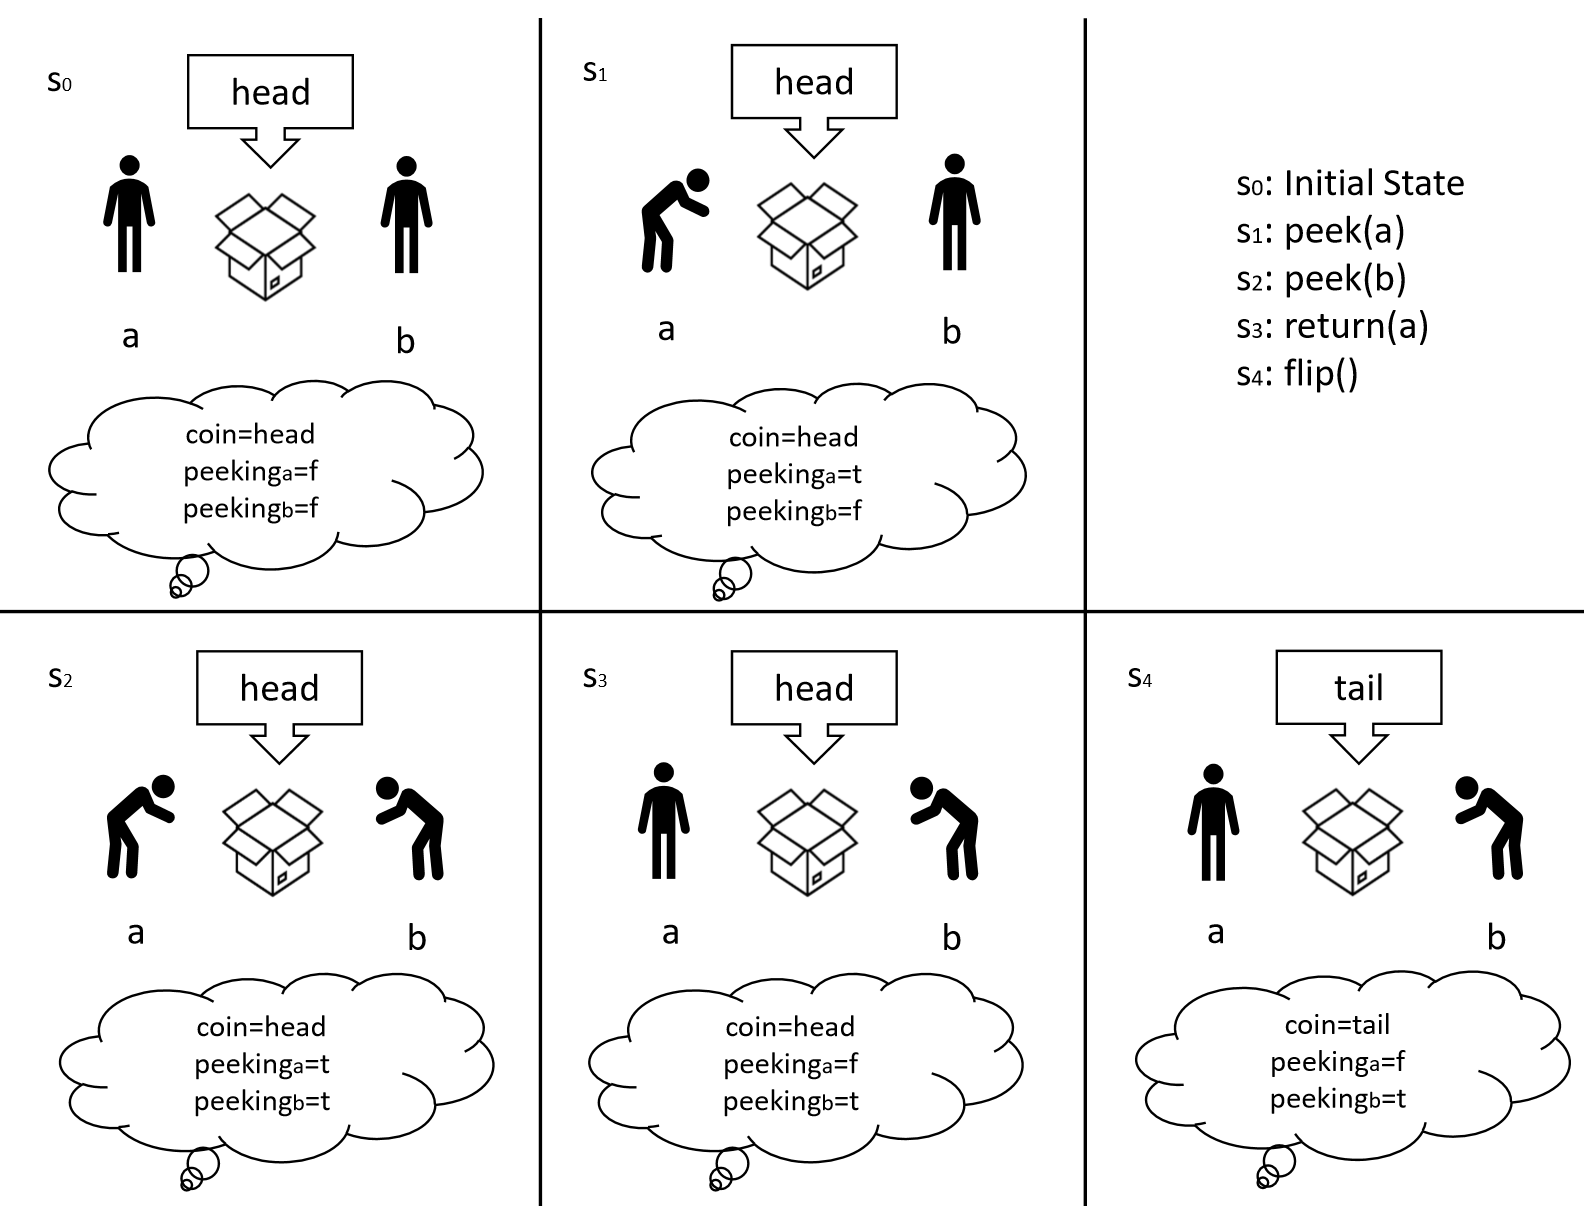
\includegraphics[width=0.9\columnwidth]{Figures/coin_plan1_s.png}
%     \caption{ The sequence of states for Plan~\ref{plan1}}
%     \label{fig:coin_plan1_s}
% \end{figure}



% Using the same example from Example~\ref{example:coin}, the state sequence $\seq=[s_0,s_1,s_2,s_3,s_4]$ from Figure~\ref{fig:coin_plan1_s} can be represented as follows:
% \begin{itemize}
%     \item [$s_0$:] $\{peeking_a \mapsto f,\ peeking_b \mapsto f,\ coin \mapsto head\}$
%     \item [$s_1$:] $\{peeking_a \mapsto t,\ peeking_b \mapsto f,\ coin \mapsto head\}$
%     \item [$s_2$:] $\{peeking_a \mapsto t,\ peeking_b \mapsto t,\ coin \mapsto head\}$
%     \item [$s_3$:] $\{peeking_a \mapsto f,\ peeking_b \mapsto t,\ coin \mapsto head\}$
%     \item [$s_4$:] $\{peeking_a \mapsto f,\ peeking_b \mapsto t,\ coin \mapsto tail\}$
% \end{itemize}

% \begin{figure}
%     \centering
%     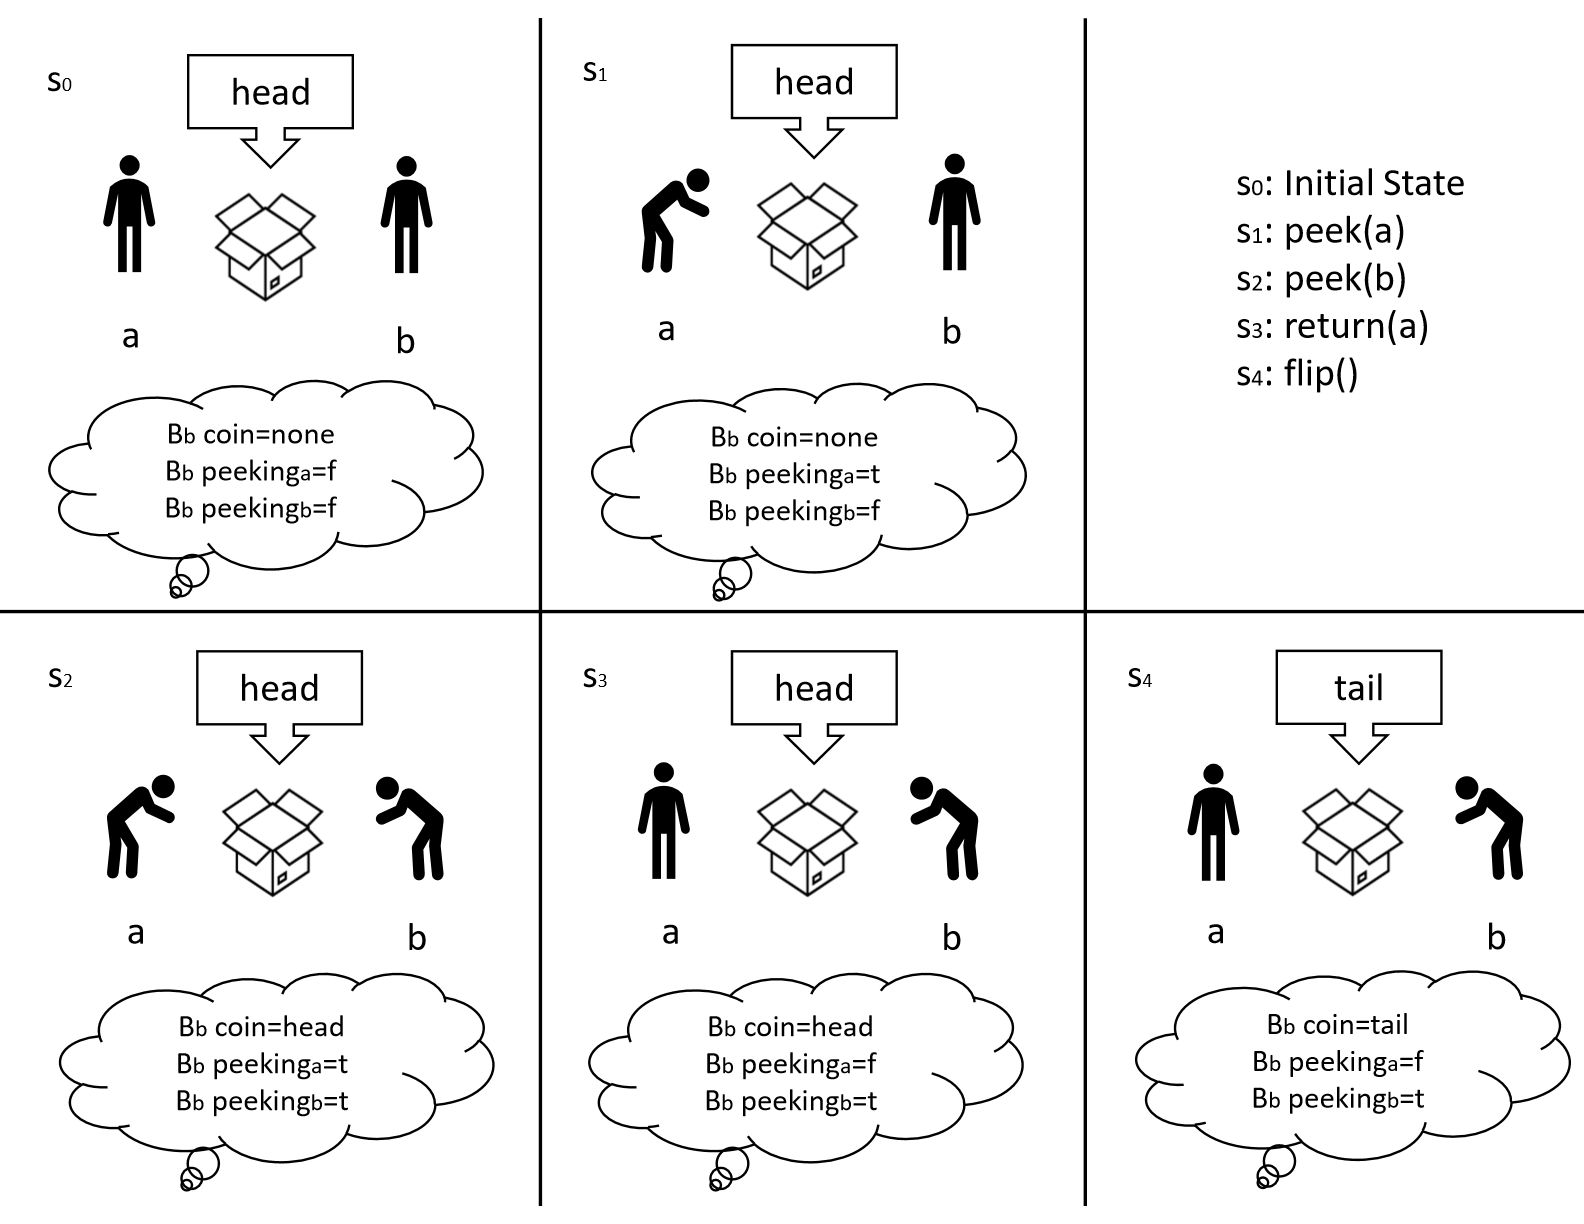
\includegraphics[width=0.9\columnwidth]{Figures/coin_plan1_sb.png}
%     \caption{ Agent $b$'s perspective for Plan~\ref{plan1}}
%     \label{fig:coin_plan1_sb}
% \end{figure}



% Agent $b$'s perspectives ($\f_b(\seq)$) should be (Figure~\ref{fig:coin_plan1_sb}):
% \begin{itemize}
%     \item [$s_0$:] $\{peeking_a \mapsto f,\ peeking_b \mapsto f,\ coin \mapsto None\}$
%     \item [$s_1$:] $\{peeking_a \mapsto t,\ peeking_b \mapsto f,\ coin \mapsto None\}$
%     \item [$s_2$:] $\{peeking_a \mapsto t,\ peeking_b \mapsto t,\ coin \mapsto head\}$
%     \item [$s_3$:] $\{peeking_a \mapsto f,\ peeking_b \mapsto t,\ coin \mapsto head\}$
%     \item [$s_4$:] $\{peeking_a \mapsto f,\ peeking_b \mapsto t,\ coin \mapsto tail\}$
% \end{itemize}
% All variables agent $b$ can see are in the red dash circles.


% \begin{figure}
%     \centering
%     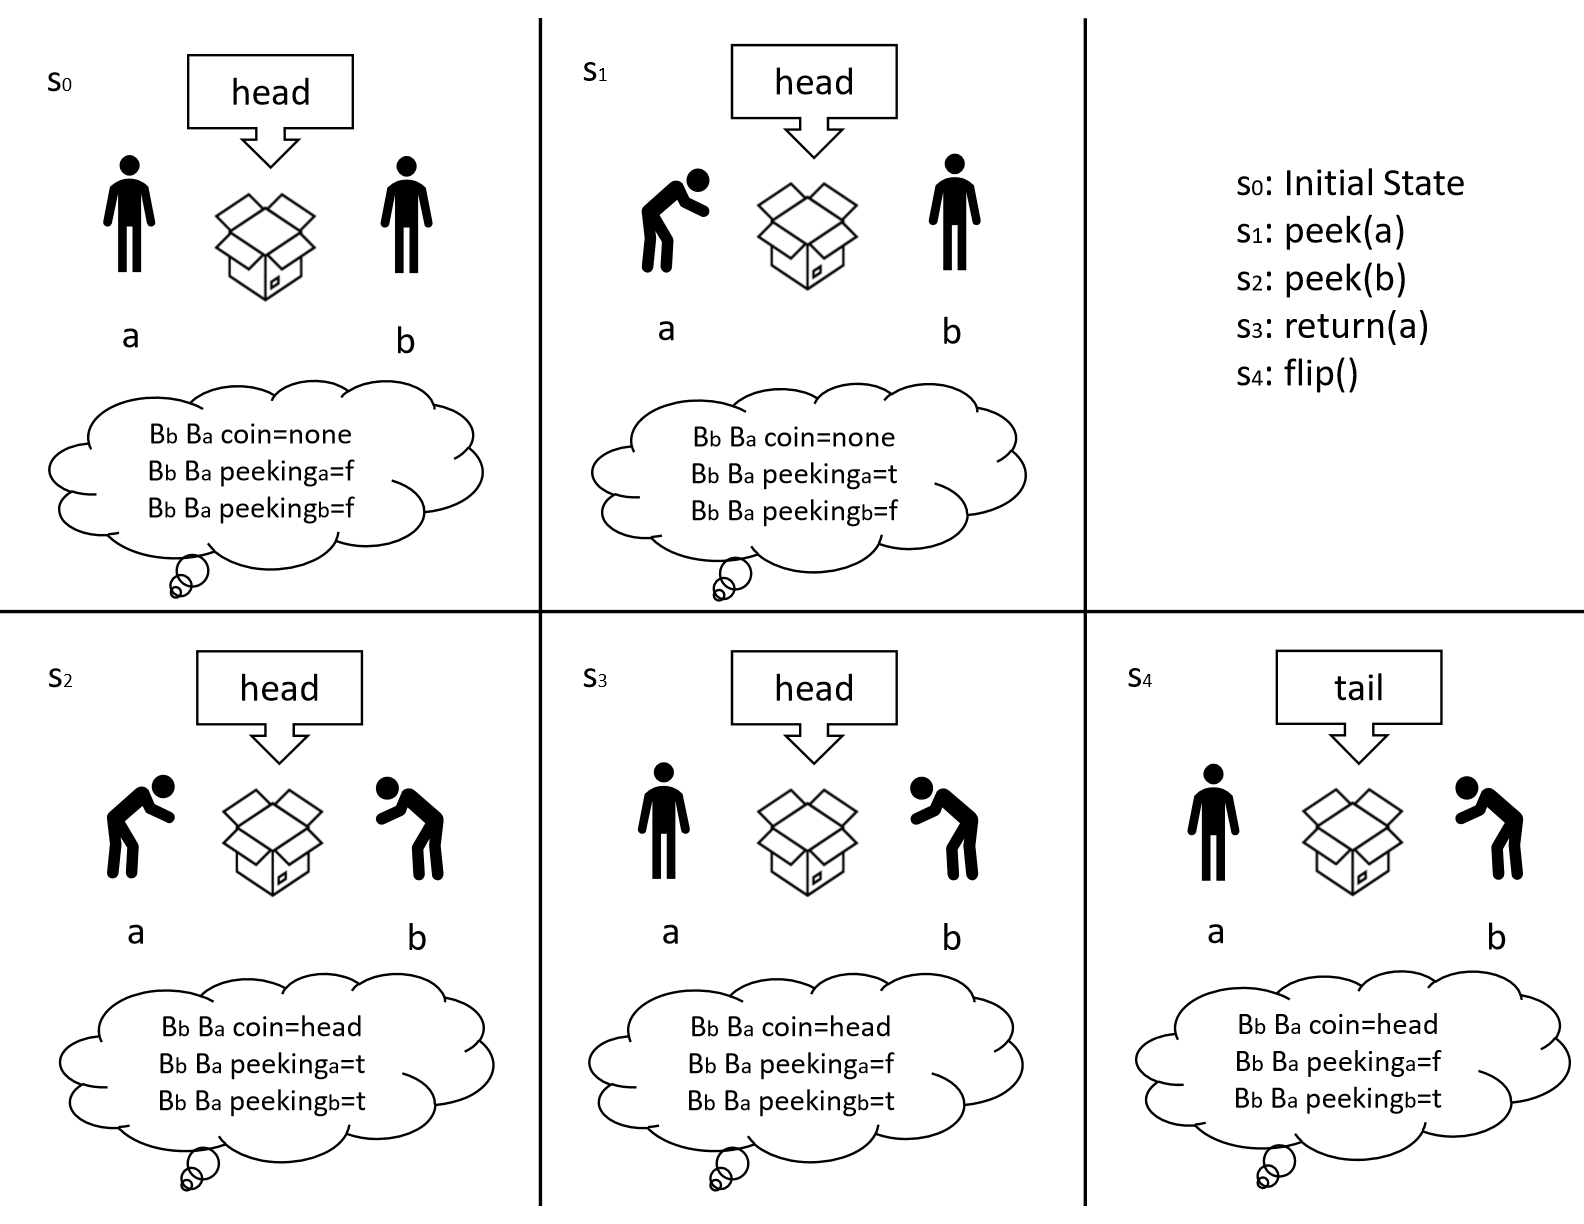
\includegraphics[width=0.9\columnwidth]{Figures/coin_plan1_sba.png}
%     \caption{ Agent $a$'s perspective under $b$'s perspective for Plan~\ref{plan1}}
%     \label{fig:coin_plan1_sba}
% \end{figure}

% In agent $b$'s mind, agent $a$'s perspectives ($\f_a(\f_b(\seq))$) should be (Figure~\ref{fig:coin_plan1_sba}):
% \begin{itemize}
%     \item [$s_0$:] $\{peeking_a \mapsto f,\ peeking_b \mapsto f,\ coin \mapsto None\}$
%     \item [$s_1$:] $\{peeking_a \mapsto t,\ peeking_b \mapsto f,\ coin \mapsto None\}$
%     \item [$s_2$:] $\{peeking_a \mapsto t,\ peeking_b \mapsto t,\ coin \mapsto head\}$
%     \item [$s_3$:] $\{peeking_a \mapsto f,\ peeking_b \mapsto t,\ coin \mapsto head\}$
%     \item [$s_4$:] $\{peeking_a \mapsto f,\ peeking_b \mapsto t,\ coin \mapsto head\}$
% \end{itemize}

% \begin{figure*}
%     \centering
%     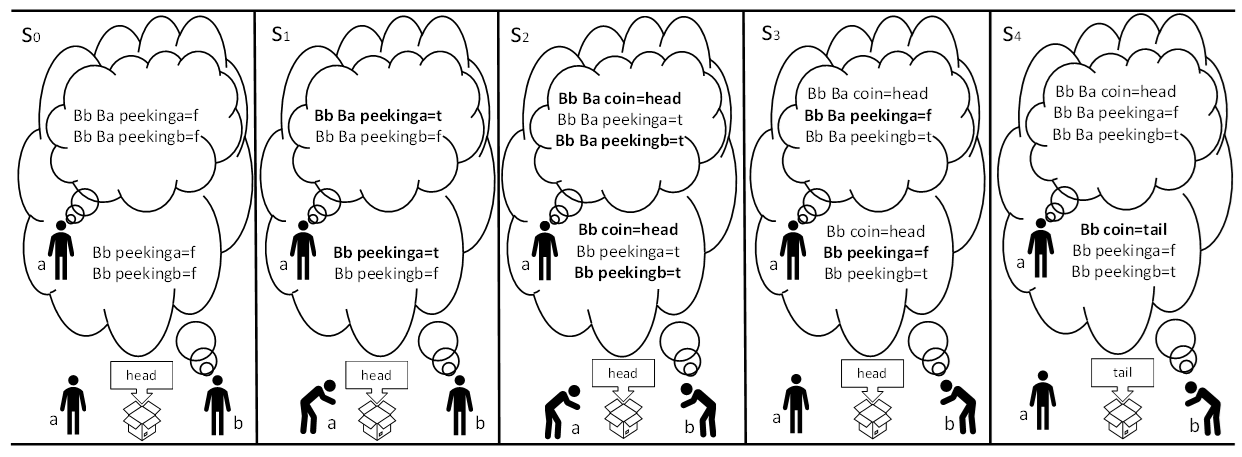
\includegraphics[width=0.9\textwidth]{Figures/plan_1_final.png}
%     \caption{Plan~\ref{plan1} with agent $b$'s justified beliefs. Bold text indicates belief that has changed.}
%     \label{fig:plan_1_final}
% \end{figure*}

Figure~\ref{fig:plan_1_final} shows the evolution of agent $b$'s justified perspective as well as agent $b$'s mind about agent $a$'s justified perspective.
Since agent $b$'s justified perspectives are derived directly from the sequence of world states $\seq$, $b$'s justified perspectives are generated simply based on $b$'s observation function.
However, the nested perspective $\f_a(\f_b(\seq))$ is worth discussing.
As both $peeking_a$ and $peeking_b$ are visible to all agents at all times, they are always common knowledge. We focus on the steps needed to retrieve the value for variable $coin$ in state $s_4$ to generate $\f_a(\f_b(\seq))$:

\begin{enumerate}
    \item Under $b$'s justified perspective $\f_b(\seq)$, finding all the timestamps ($a\timestamp$) that agent $a$ sees $coin$. The set of timestamps $ts = \{1,2\}$.
    \item Identifying the latest timestamp ($lt$) that agent $a$ sees $coin$ in $\f_b(\seq)$, which is $2$. 
    \item  $\memorization(\f_b(\seq),2,coin) = \f_b(\seq)[2](coin)=head$ since $coin\in \f_b(\seq)[2]$ and $b$'s perspective of $coin$ at this time is $head$.. 
\end{enumerate}
\end{example}

\end{comment}

\begin{example}[Example~\ref{example:coin} with Plan~\ref{plan2}]

% \begin{figure}
%     \centering
%     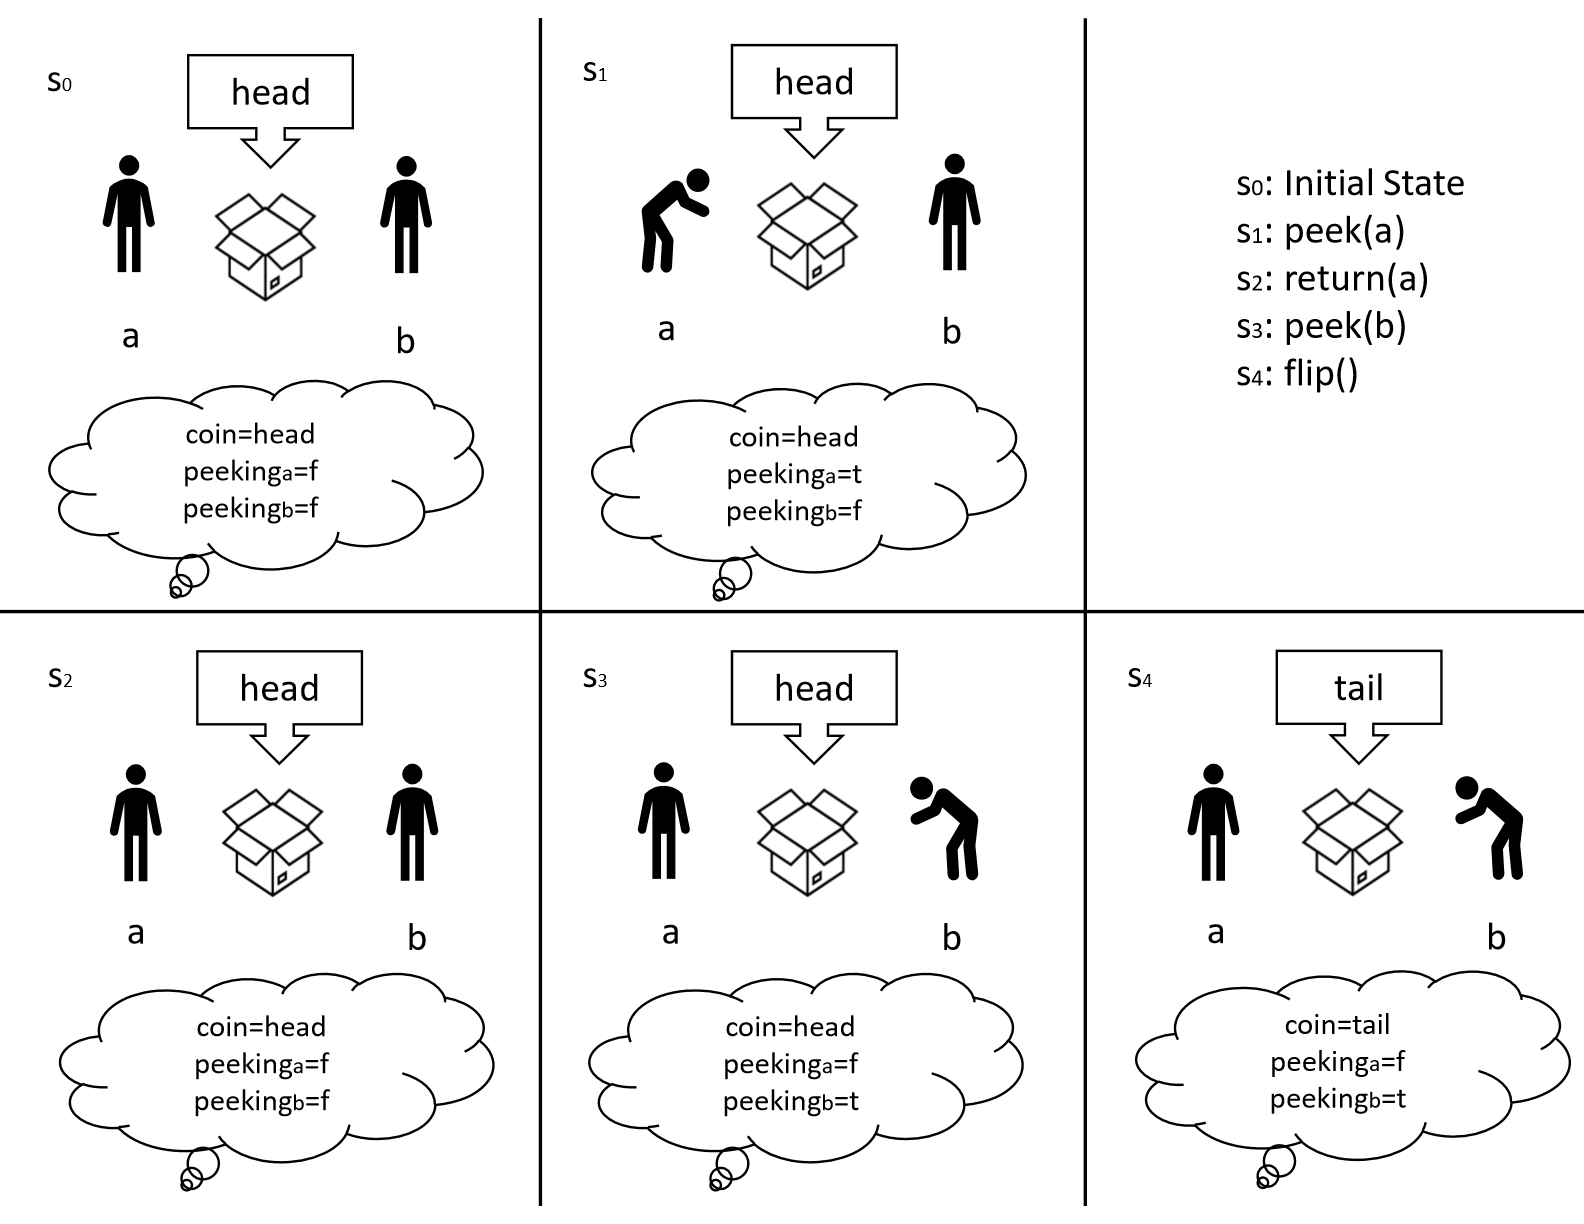
\includegraphics[width=0.9\columnwidth]{Figures/coin_plan2_s.png}
%     \caption{The sequence of states for Plan~\ref{plan2}}
%     \label{fig:coin_plan2_s}
% \end{figure}

% Let the sequence of states generated by this plan as $\seq = s_0,s_1,s_2,s_3,s_4$ (shown in Figure~\ref{fig:coin_plan2_s}).


% \begin{figure}
%     \centering
%     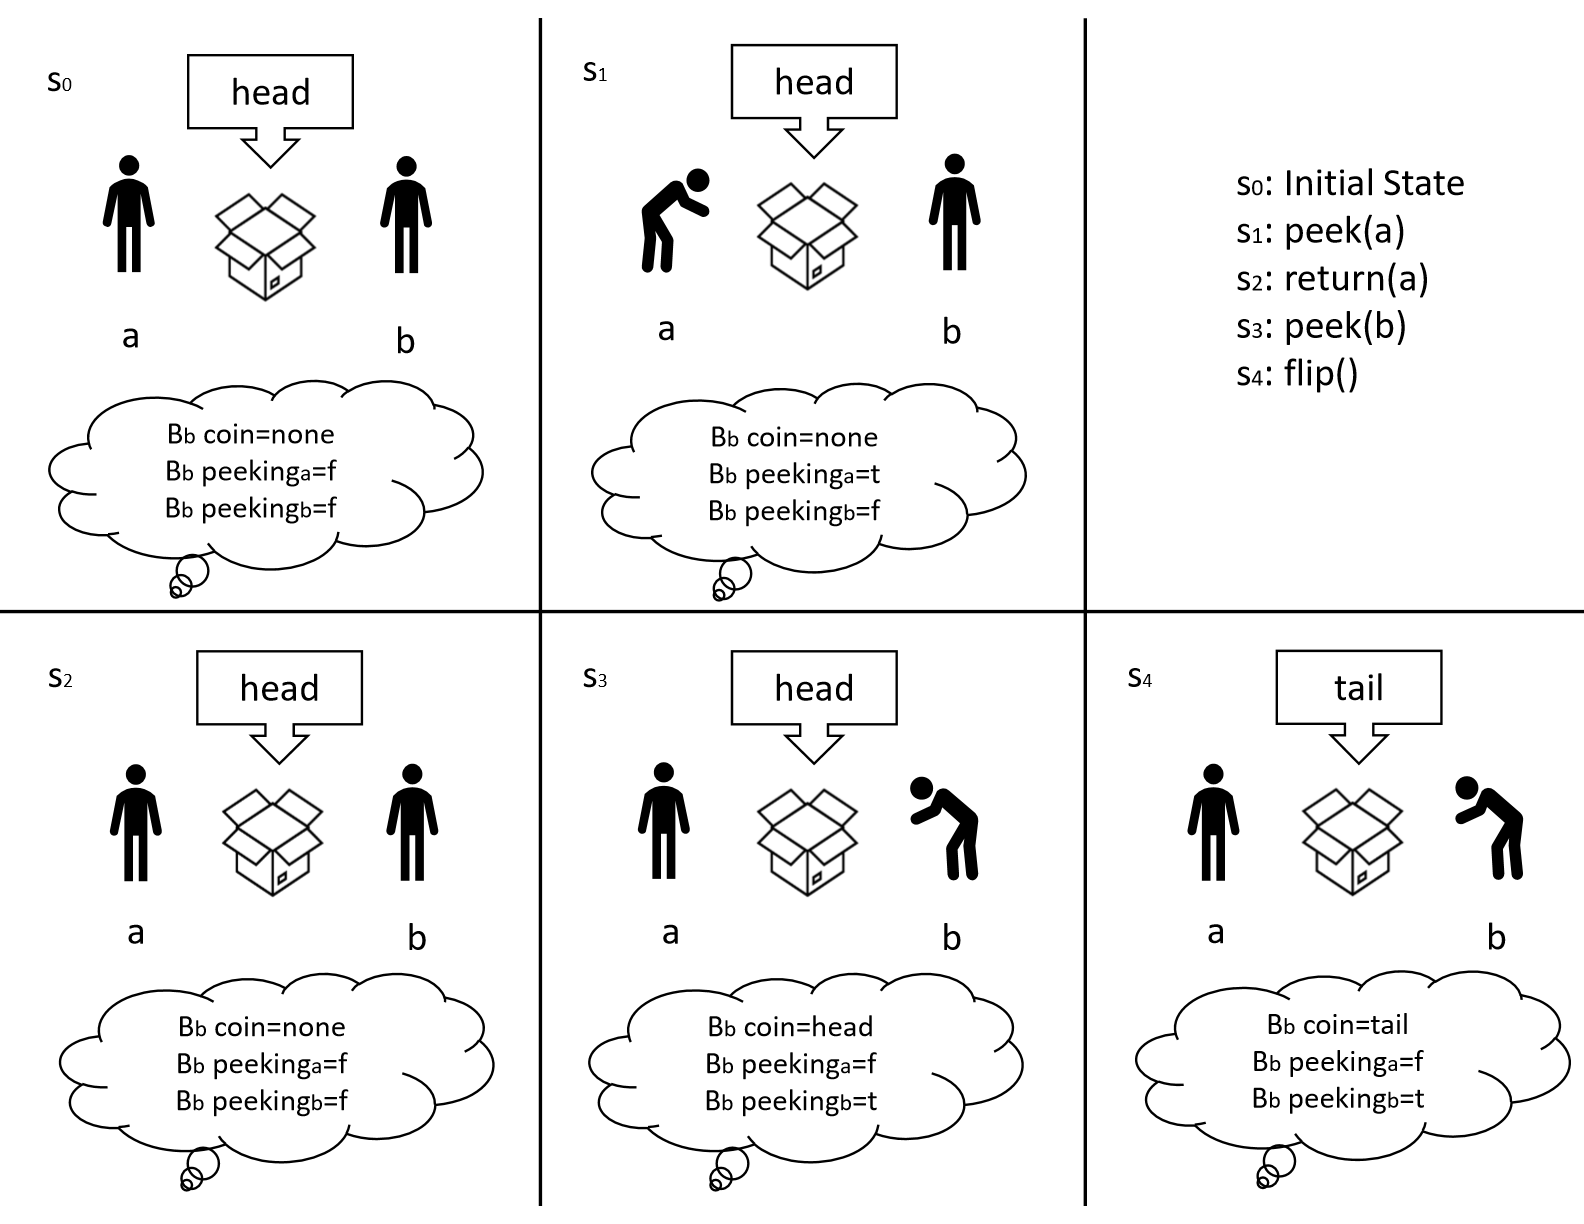
\includegraphics[width=0.9\columnwidth]{Figures/coin_plan2_sb.png}
%     \caption{ Agent $b$'s perspective for Plan~\ref{plan2}}
%     \label{fig:coin_plan2_sb}
% \end{figure}



% Agent $b$'s perspectives $\f_b(\seq)$ (shown in Figure~\ref{coin_plan2_sb}) should be:
% \begin{itemize}
%     \item [$s_0$:] $\{peeking_a \mapsto f,\ peeking_b \mapsto f,\ coin \mapsto None\}$
%     \item [$s_1$:] $\{peeking_a \mapsto t,\ peeking_b \mapsto f,\ coin \mapsto None\}$
%     \item [$s_2$:] $\{peeking_a \mapsto f,\ peeking_b \mapsto f,\ coin \mapsto None\}$
%     \item [$s_3$:] $\{peeking_a \mapsto f,\ peeking_b \mapsto t,\ coin \mapsto head\}$
%     \item [$s_4$:] $\{peeking_a \mapsto f,\ peeking_b \mapsto t,\ coin \mapsto tail\}$
% \end{itemize}

% \begin{figure}
%     \centering
%     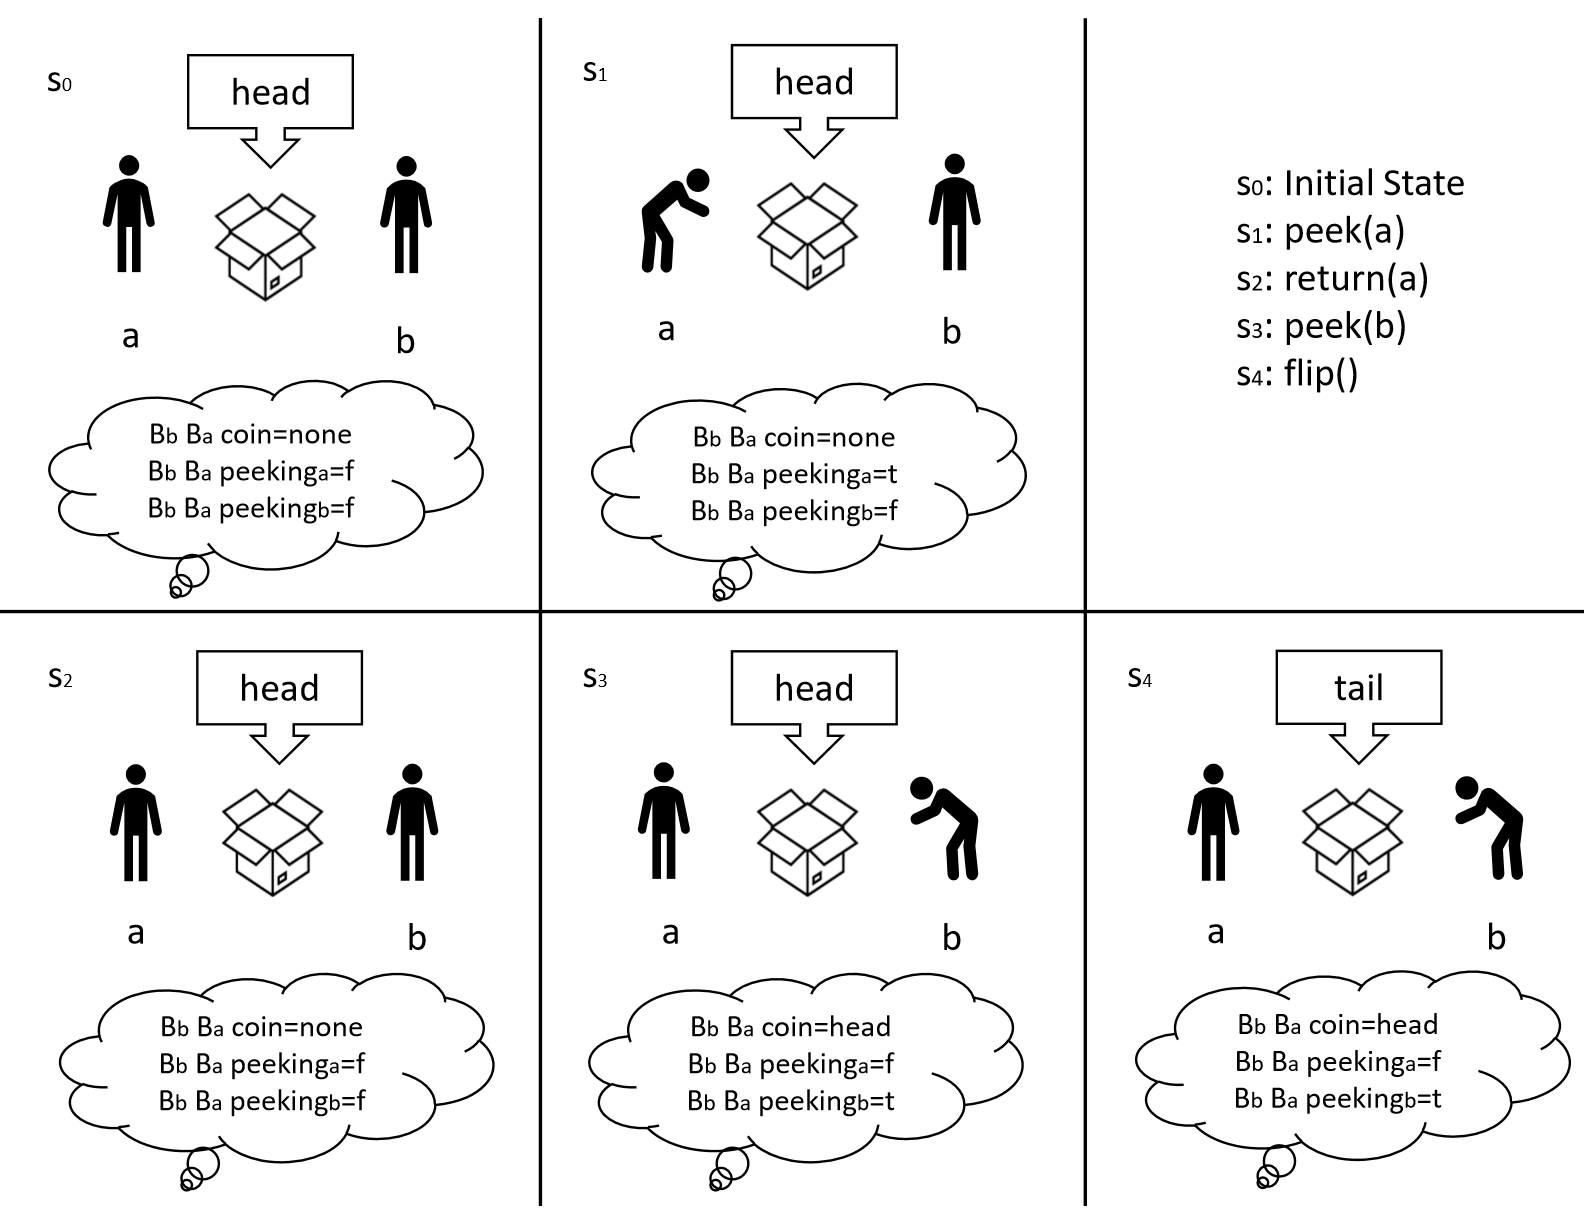
\includegraphics[width=0.9\columnwidth]{Figures/coin_plan2_sba.png}
%     \caption{ Agent $a$'s perspective under $b$'s perspective for Plan~\ref{plan2}}
%     \label{fig:coin_plan2_sba}
% \end{figure}



% In agent $b$'s mind, agent $a$'s perspectives $\f_a(\f_b(\seq))$ (shown in Figure~\ref{fig:coin_plan2_sb}) should be:
% \begin{itemize}
%     \item [$s_0$:] $\{peeking_a \mapsto f,\ peeking_b \mapsto f,\ coin \mapsto None\}$
%     \item [$s_1$:] $\{peeking_a \mapsto t,\ peeking_b \mapsto f,\ coin \mapsto None\}$
%     \item [$s_2$:] $\{peeking_a \mapsto f,\ peeking_b \mapsto f,\ coin \mapsto None\}$
%     \item [$s_3$:] $\{peeking_a \mapsto f,\ peeking_b \mapsto t,\ coin \mapsto head\}$
%     \item [$s_4$:] $\{peeking_a \mapsto f,\ peeking_b \mapsto t,\ coin \mapsto head\}$
% \end{itemize}

% \tm{I think what you have illustrated in the figures is very nice; but you need to do something other than use colours. Some people print in black and white; some are heavily colourblind. Why not just have this figure once and write $B_a coin=head$, etc. under each agent in each state? That will take up a similar amount of room, but then the beliefs, including nested beliefs, will be explicit and easy to understand}
% \gh{Updated}
% \begin{figure}
%     \centering
%     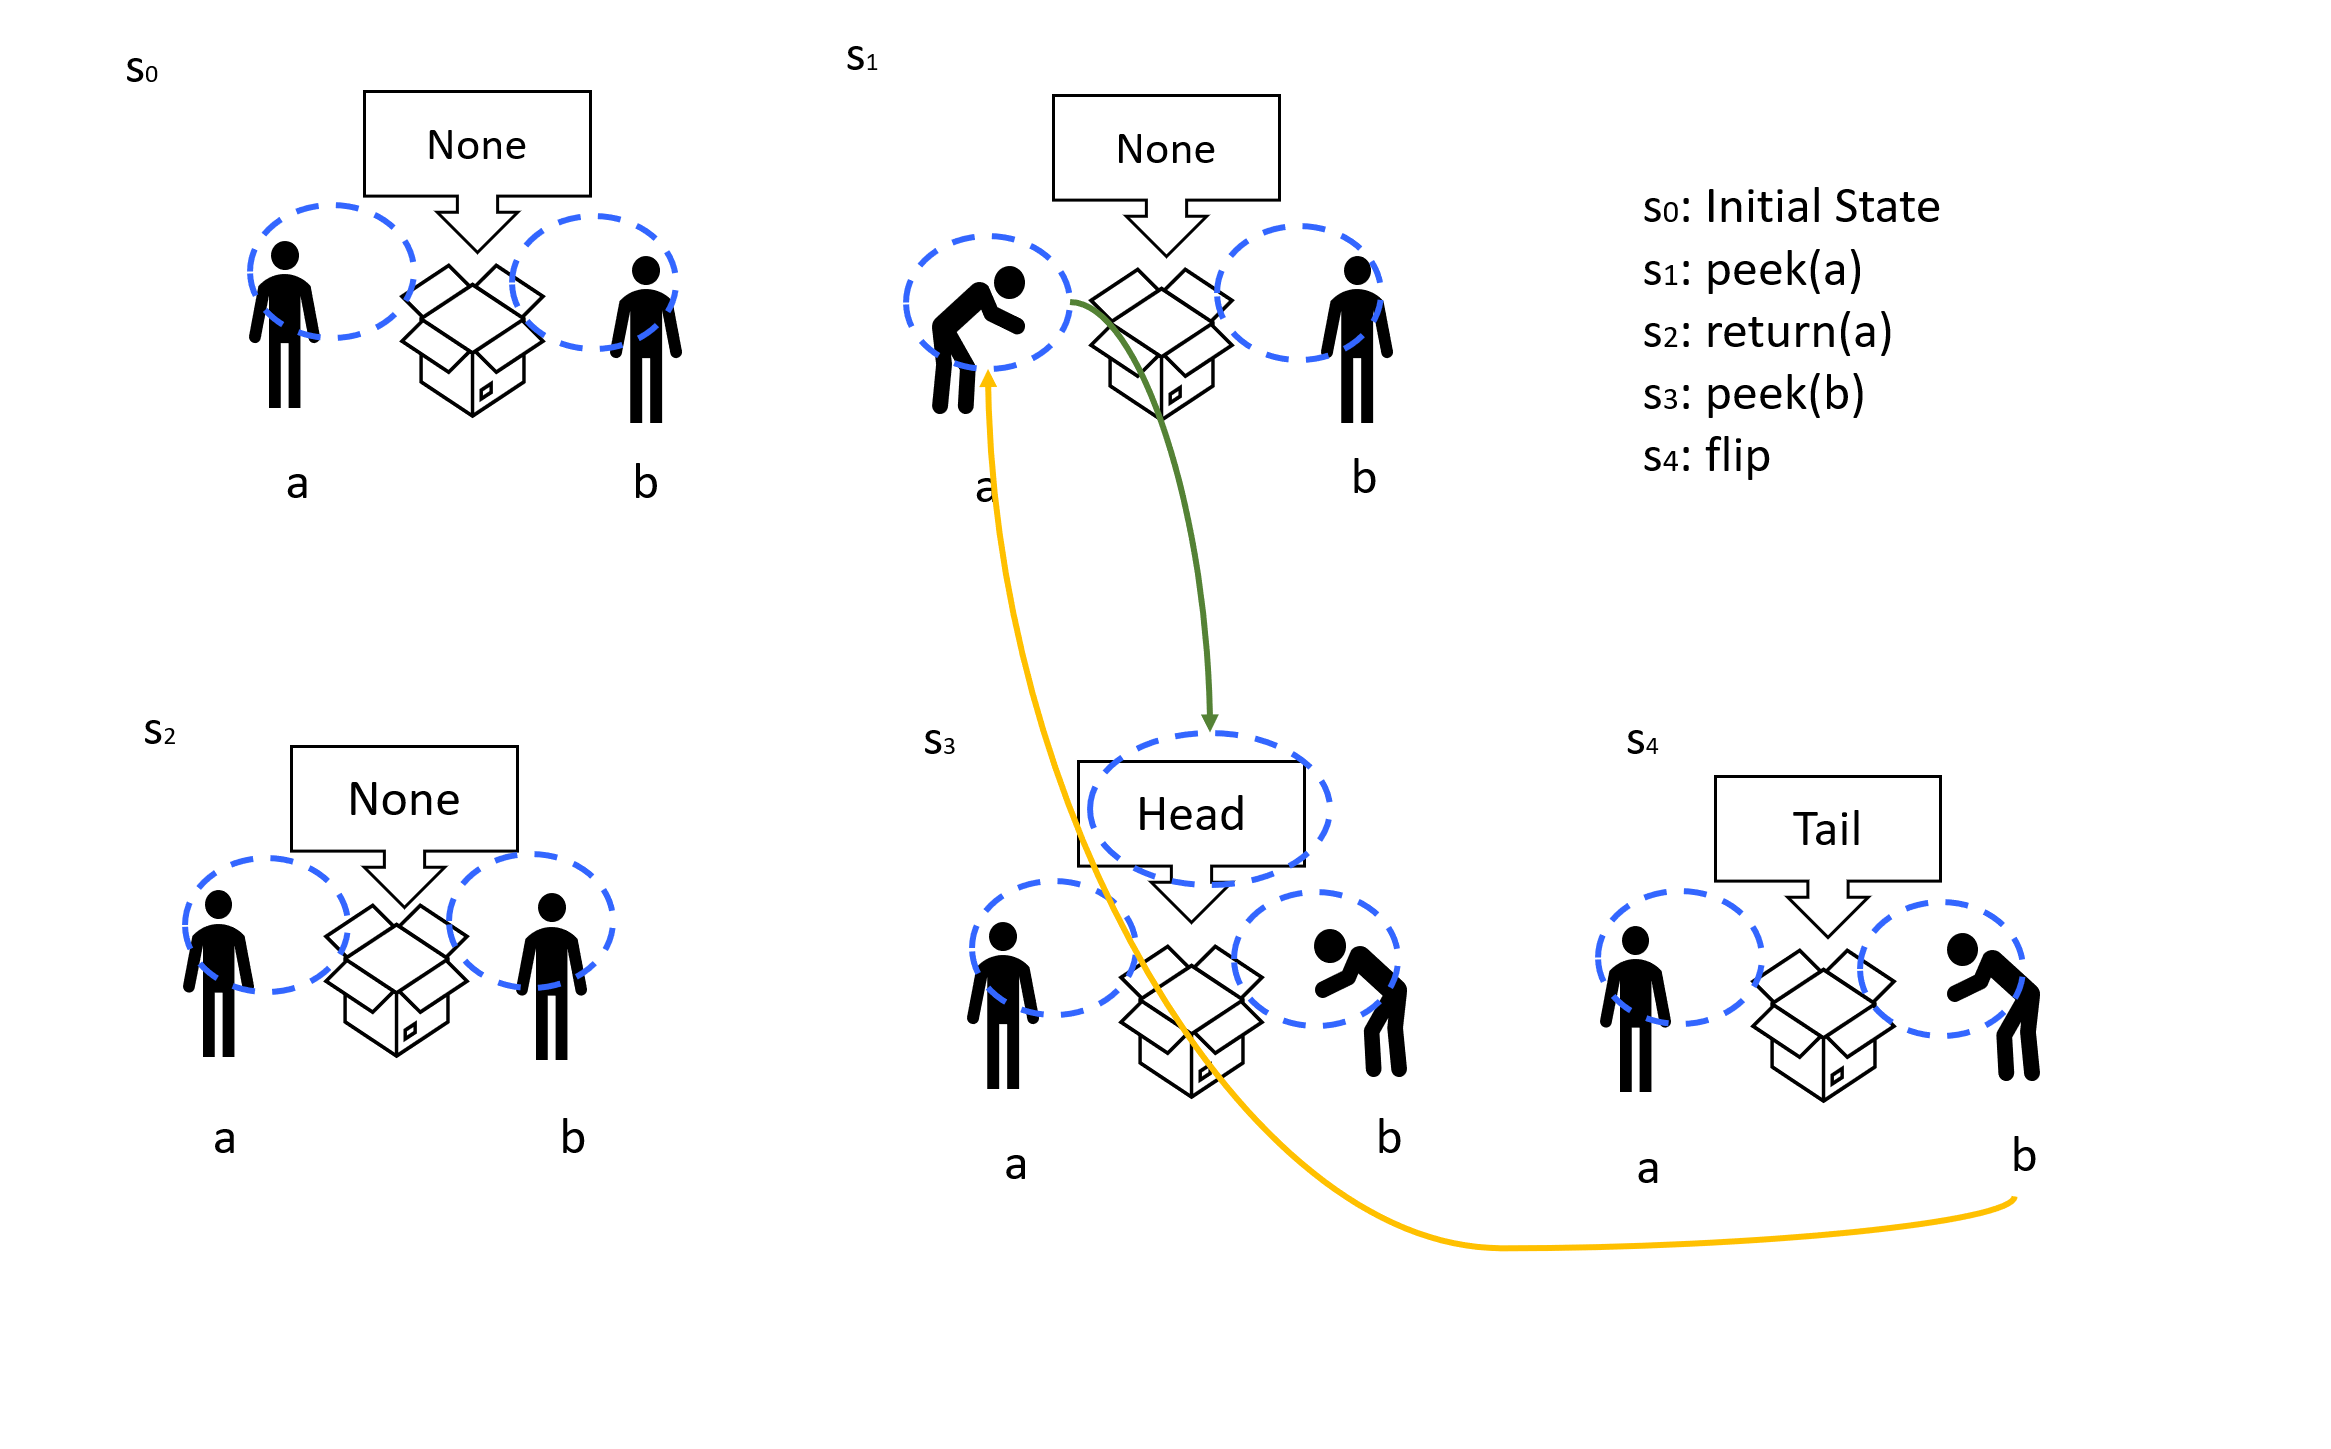
\includegraphics[width=0.9\columnwidth]{Figures/coin_example_2_ba.png}
%     \caption{ Agent $a$'s perspective under agent $b$'s perspective }
%     \label{fig:coin_example2_ba}
% \end{figure}

% \begin{figure*}
%     \centering
%     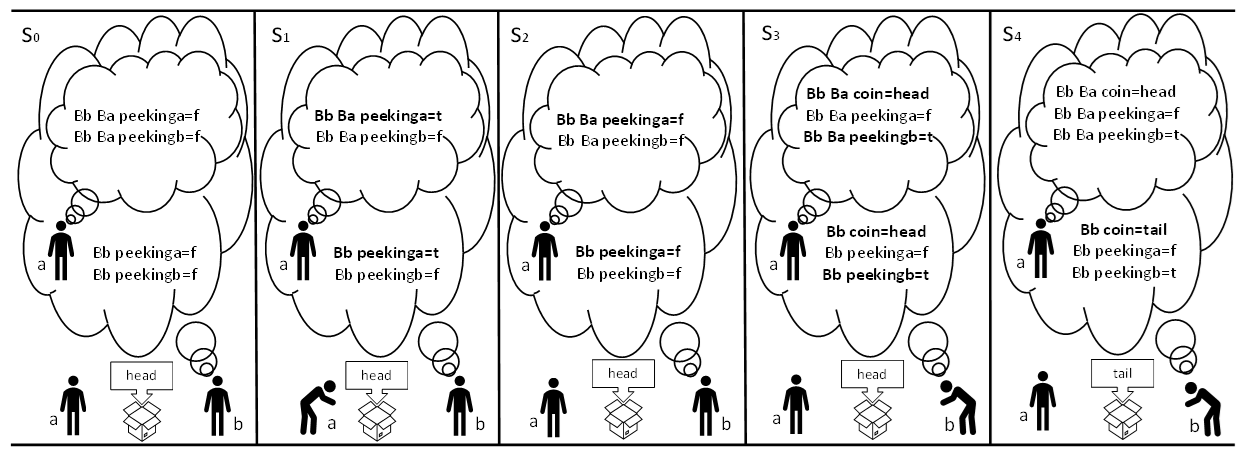
\includegraphics[width=0.9\textwidth]{Figures/plan_2_final.png}
%     \caption{Plan~\ref{plan2} with agent $b$'s justified beliefs. Bold text indicates belief that has changed.}
%     \label{fig:plan_2_final}
% \end{figure*}


In Figure~\ref{fig:plan_2_final}, agent $b$ cannot at the same time: 1) see agent $a$ peeking into the box and 2) see what was inside the box at that time, because $a$ and $b$ are no longer peeking into the box at the same time, as they were in $s_2$ from Plan~\ref{plan1}.
The latest timestamp $lt$ agent $a$ peeked into the box is $1$.
We can retrieve the value of the $coin$ at timestamp 1 from $b$'s perspective using $\memorization(\seq,1,coin)$.
In agent $b$'s perspective, there is no information about $coin$ until $s_3$, making the return value of $\memorization(\seq,1,coin)$ to be $\f_b(s)[3](coin)=head$.
% In agent $b$'s perspective, there is no information about $coin$ until $s_3$, so in $\memorization(\seq,1,coin)$, we have that the value of $coin$ is $head$ in $\f_b(\seq)$ at timestamp $3$.
So, $M,\seq \vDash B_b B_a coin=head$ is equivalent to $M,\f_b(\seq) \vDash B_a coin=head $, which is $M,\f_a(\f_b(\seq)) \vDash coin=head$.
Therefore, the justified belief of agent $b$ on a false belief about agent $a$ on $\varphi$ can be generated even if $b$ cannot see both 1) the truth value of $\varphi$ while 2) seeing agent $a$ seeing $\varphi$ at the same timestamp (same state).
\end{example}








% \subsection{BBL}
% BBL is a domain that contains stationary cameras that can turn or observe a certain range in a 2-dimension plane. Let there be two agents (cameras) $a$, $b$, and one movable proposition $p$. Initially ($s_0$), both $a$ can see both $b$ and $p$, while $b$ can see only $p$.

% \begin{figure*}[ht]
%     \centering
%     % % \begin{tikzpicture}
% %   \matrix (m) [matrix of math nodes,row sep=3em,column sep=4em,minimum width=2em]
% %   {
% %      F_t(x) & F(x) \\
% %      A_t & A \\};
% %   \path[-stealth]
% %     (m-1-1) edge node [left] {$\mathcal{B}_X$} (m-2-1)
% %             edge [double] node [below] {$\mathcal{B}_t$} (m-1-2)
% %     (m-2-1.east|-m-2-2) edge node [below] {$\mathcal{B}_T$}
% %             node [above] {$\exists$} (m-2-2)
% %     (m-1-2) edge node [right] {$\mathcal{B}_T$} (m-2-2)
% %             edge [dashed,-] (m-2-1);
% % \end{tikzpicture}


% \newcommand{\scale}{0.4}
% \newcommand{\range}{30}
% \newcommand{\size}{3}
% \newcommand{\oversize}{6}
% \makeatletter
% \newcommand{\gettikzxy}[3]{%
%   \tikz@scan@one@point\pgfutil@firstofone#1\relax
%   \edef#2{\the\pgf@x}%
%   \edef#3{\the\pgf@y}%
% }
% \makeatother

% \begin{tikzpicture}
%     \coordinate (top_left) at (0,20*\scale);
%     \coordinate (bottom_left) at (0,0);
%     \coordinate (top_right) at (20*\scale,20*\scale);
%     \coordinate (bottom_right) at (20*\scale,0);

%     \coordinate (origin) at (0,0);
%     \coordinate (a1) at (5*\scale,5*\scale);
%     \coordinate (a1_up) at (5*\scale,20*\scale);
%     \coordinate (a1_down) at (20*\scale,5*\scale);
%     \coordinate (a1_dir) at (6*\scale,6*\scale);
%     \coordinate (a2) at (15*\scale,15*\scale);
%     \coordinate (a2_up) at (0,15*\scale);
%     \coordinate (a2_down) at (15*\scale,0);
%     \coordinate (a2_dir) at (14*\scale,14*\scale);
        
%     \begin{scope}[transparency group]
%         \begin{scope}[blend mode=multiply]
%             \fill[ opacity=0.5,blue!30] (a1) -- (a1_up) -- (top_right) -- (a1_down) -- cycle;
%             \fill[ opacity=0.5,yellow!30] (a2) -- (a2_up) -- (bottom_left) -- (a2_down) -- cycle;
%         \end{scope}
%     \end{scope}
    
%     \draw[thick, black,->] (a1) -- (a1_dir);
%     \draw[thick, black,->] (a2) -- (a2_dir);
    

%     \draw[thick] let    \p{1} = (a1)    in (a1 |- origin)
%         node[circle,fill=red!80,inner sep=2pt,
%         label={[align=center]below:
%                 $a_1$ \\ 
%                 (\pgfmathparse{(\x1/28.45274)}\num[round-mode=places,round-precision=1]{\pgfmathresult},
%                 \pgfmathparse{(\y1/28.45274)}\num[round-mode=places,round-precision=1]{\pgfmathresult})
%                 }] at (\x1,\y1) {};
%     \draw[->, black] (a1) -- (a1_up);
%     \draw[->, black] (a1) -- (a1_down);
    
                
%     \draw[thick] let    \p{1} = (a2)    in (a1 |- origin)
%         node[circle,fill=red!80,inner sep=2pt,
%         label={[align=center]below:
%                 $a_2$ \\ 
%                 (\pgfmathparse{(\x1/28.45274)}\num[round-mode=places,round-precision=1]{\pgfmathresult},
%                 \pgfmathparse{(\y1/28.45274)}\num[round-mode=places,round-precision=1]{\pgfmathresult})
%                 }] at (\x1,\y1) {};
%     \draw[->, black] (a2) -- (a2_up);
%     \draw[->, black] (a2) -- (a2_down);
    
    
%     % border

    
%     \draw[black] (top_left) -- (bottom_left) -- (bottom_right) -- (top_right) -- cycle;

    
%     % \draw[->, gray, thick] ({cos(\range)*\size*2},0) -- ({cos(\range)*\size*2-cos(\range)*\oversize},{sin(\range)*\oversize});
%     % \draw[->, gray, thick] ({cos(\range)*\size*2},0) -- ({cos(\range)*\size*2},0) -- ({cos(\range)*\size*2-cos(\range)*\oversize},-{sin(\range)*\oversize});
    
    
%     \coordinate (b1) at (10*\scale,10*\scale);
%     \coordinate (b2) at (2.5*\scale,2.5*\scale);
%     \coordinate (b3) at (17.5*\scale,17.5*\scale);
    
%     \draw[thick] let    \p{1} = (b1)    in (a1 |- origin)
%         node[circle,fill=black!80,inner sep=1pt,
%         label={[align=center]below:
%                 $b_1$ \\ 
%                 (\pgfmathparse{(\x1/28.45274)}\num[round-mode=places,round-precision=1]{\pgfmathresult},
%                 \pgfmathparse{(\y1/28.45274)}\num[round-mode=places,round-precision=1]{\pgfmathresult})
%                 }] at (\x1,\y1) {};
                
%     \draw[thick] let    \p{1} = (b2)    in (a1 |- origin)
%         node[circle,fill=black!80,inner sep=1pt,
%         label={[align=center]below:
%                 $b_2$ \\ 
%                 (\pgfmathparse{(\x1/28.45274)}\num[round-mode=places,round-precision=1]{\pgfmathresult},
%                 \pgfmathparse{(\y1/28.45274)}\num[round-mode=places,round-precision=1]{\pgfmathresult})
%                 }] at (\x1,\y1) {};    

%     \draw[thick] let    \p{1} = (b3)    in (a1 |- origin)
%         node[circle,fill=black!80,inner sep=1pt,
%         label={[align=center]below:
%                 $b_3$ \\ 
%                 (\pgfmathparse{(\x1/28.45274)}\num[round-mode=places,round-precision=1]{\pgfmathresult},
%                 \pgfmathparse{(\y1/28.45274)}\num[round-mode=places,round-precision=1]{\pgfmathresult})
%                 }] at (\x1,\y1) {};    
                
%     % \filldraw[black] ({cos(\range)*\size},0) circle (2pt) node[anchor=west] {$b_2$};
%     % \filldraw[black] (-{cos(\range)*\size},0) circle (2pt) node[anchor=west] {$b_1$};
%     % \filldraw[black] ({cos(\range)*\size*3},0) circle (2pt) node[anchor=west] {$b_3$};
%     % \filldraw[black] ({cos(\range)*\size},{sin(\range)*\oversize*3/4}) circle (2pt) node [anchor=west] {$b_4$};
    

    
    
%     % border
%     % \draw[gray, thick] (-{cos(\range)*\size*2},-{sin(\range)*\oversize}) -- ({cos(\range)*\size*4},-{sin(\range)*\oversize});
%     % \draw[gray, thick] (-{cos(\range)*\size*2},{sin(\range)*\oversize}) -- ({cos(\range)*\size*4},{sin(\range)*\oversize});
%     % \draw[gray, thick] ({cos(\range)*\size*4},{sin(\range)*\oversize}) -- ({cos(\range)*\size*4},-{sin(\range)*\oversize});
%     % \draw[gray, thick] (-{cos(\range)*\size*2},{sin(\range)*\oversize}) -- (-{cos(\range)*\size*2},-{sin(\range)*\oversize});
% \end{tikzpicture}

% % \begin{tikzpicture}
% %     %\draw [help lines] (0,0) grid (4,4);
% %     %\coordinate (origin) at (0,0);
% %     \node[circle,fill]  (d1) at (3,2) {};

% %     %\draw[red,thick] let    \p{1} = (d1)    in (d1|- origin) node[label=below:$\x1$]{} --  (d1) --  (d1 -| origin) node[label=left:\y1]{} ;

% %     \end{tikzpicture}




% \begin{tikzpicture}
%   \matrix (m) [matrix of math nodes,row sep=3em,column sep=4em,minimum width=2em]
%   {
%      F_t(x) & F(x) \\
%      A_t & A \\};
%   \path[-stealth]
%     (m-1-1) edge node [left] {$\mathcal{B}_X$} (m-2-1)
%             edge [double] node [below] {$\mathcal{B}_t$} (m-1-2)
%     (m-2-1.east|-m-2-2) edge node [below] {$\mathcal{B}_T$}
%             node [above] {$\exists$} (m-2-2)
%     (m-1-2) edge node [right] {$\mathcal{B}_T$} (m-2-2)
%             edge [dashed,-] (m-2-1);
% \end{tikzpicture}


\newcommand{\scale}{0.4}
\newcommand{\range}{30}
\newcommand{\size}{3}
\newcommand{\oversize}{6}
\makeatletter
\newcommand{\gettikzxy}[3]{%
  \tikz@scan@one@point\pgfutil@firstofone#1\relax
  \edef#2{\the\pgf@x}%
  \edef#3{\the\pgf@y}%
}
\makeatother

\begin{tikzpicture}
    \coordinate (top_left) at (0,20*\scale);
    \coordinate (bottom_left) at (0,0);
    \coordinate (top_right) at (20*\scale,20*\scale);
    \coordinate (bottom_right) at (20*\scale,0);

    \coordinate (origin) at (0,0);
    \coordinate (a1) at (10*\scale,10*\scale);
    \coordinate (a1_up) at (0*\scale,10*\scale);
    \coordinate (a1_down) at (10*\scale,0*\scale);
    \coordinate (a1_opp) at (0*\scale,0*\scale);
    
    \coordinate (a1_dir) at (9*\scale,9*\scale);
    
    \coordinate (a2) at (15*\scale,15*\scale);
    \coordinate (a2_up) at (0,15*\scale);
    \coordinate (a2_down) at (15*\scale,0);
    \coordinate (a2_dir) at (14*\scale,14*\scale);
    

    \coordinate (b2) at (5*\scale,5*\scale);
    
        
    \begin{scope}[transparency group]
        \begin{scope}[blend mode=multiply]
            \fill[ opacity=0.5,blue!30] (a1) -- (a1_up) -- (a1_opp) -- (a1_down) -- cycle;
            \fill[ opacity=0.5,yellow!30] (a2) -- (a2_up) -- (bottom_left) -- (a2_down) -- cycle;
        \end{scope}
    \end{scope}
    
    \draw[thick, black,->] (a1) -- (a1_dir);
    \draw[thick, black,->] (a2) -- (a2_dir);
    

    \draw[thick] let    \p{1} = (a1)    in (a1 |- origin)
        node[circle,fill=red!80,inner sep=2pt,
        label={[align=center, xshift=0.6cm]below:
                $b$ \\ 
                (10,10)
                }] at (\x1,\y1) {};
    \draw[->, black] (a1) -- (a1_up);
    \draw[->, black] (a1) -- (a1_down);
    
                
    \draw[thick] let    \p{1} = (a2)    in (a1 |- origin)
        node[circle,fill=red!80,inner sep=2pt,
        label={[align=center, xshift=0.5cm]below:
                $a$ \\ 
                (15,15)
                }] at (\x1,\y1) {};
    \draw[->, black] (a2) -- (a2_up);
    \draw[->, black] (a2) -- (a2_down);
    
    
    % border

    
    \draw[black] (top_left) -- (bottom_left) -- (bottom_right) -- (top_right) -- cycle;
    
    

    
                
    \draw[thick] let    \p{1} = (b2)    in (a1 |- origin)
        node[circle,fill=black!80,inner sep=1pt,
        label={[align=center]above:
                $c$ \\ 
                (5,5)
                }] at (\x1,\y1) {};    

                
\end{tikzpicture}

%     \caption{Example for Big Brother Logic}
%     \label{fig:big_brother_exp}
% \end{figure*}

% \subsubsection{Initial State}
% Firstly, in order to model this domain into state, we need to have variables that represents the directions of the agents: $dir(a)$ and $dir(b)$, and the location of the proposition $loc(p)$. Since all agents are stationary, with the information of the direction, it is easy to calculate whether an agent can see something or not based on the line of sight in the perspective functions. Then, initially, the global state and agent's local state should be $\{dir(a),dir(b),loc(p),p\}$, $\{dir(a),dir(b),loc(p),p\}$ and $\{dir(a)=null,dir(b),loc(p),p\}$ respectively. And clearly, we have the following epistemic relations:
% \begin{itemize}
%     \item $K_a p$, $K_b p$
%     \item $K_a K_b p$, $\neg K_b K_a p$ ($\neg S_b S_a p$)
%     \item $B_a p$, $B_b p$
%     \item $K_a B_b p$, $\neg K_b B_a p$
%     \item $B_a B_b p$, $\neg B_b B_a p$
% \end{itemize}

% \subsubsection{State 1}
% Then, we rotate the direction of the agent $b$ by $180_{\circ} $ so that he could see $a$, but cannot see $p$. We note this state as $s1$ and $b$'s direction as $dir(b)'$. Then, we have each agents observation as $\{dir(a),dir(b)',loc(p),p\}$ and $\{dir(b)',dir(a)\}$ respectively. In the meantime, $\memorization_b(s_1)$ = $\f_b(s_0) \backslash \observation_b(s_1) = \{loc(p),p\}$.
% Based on their perspectives, we have:

% \begin{itemize}
%     \item $K_a p$, $\neg K_b p$
%     \item $K_a \neg K_b p$ ($K_a \neg S_b p$), $\neg K_b K_a p$ ($\neg S_b p$)
%     \item $B_a p$, $B_b p$
%     \item $K_a B_b p$, $\neg K_b B_a p$ ($\neg S_b p$)
%     \item $B_a B_b p$, $B_b B_a p$
% \end{itemize}

% Most of the above epistemic formulae are trivial, except $\neg K_b B_a p$, $B_b B_a p$ and $B_a B_b p$. For agent $b$, in order to see $B_a p$, he need to see all the variables that related to the evaluation of the formula, which includes $p$ and $dir(a)$. Since $\neg S_b p$, then we have $\neg K_b B_a p$. 
% As for $B_b B_a p$, $(M,s_1) \vDash B_b B_a p$ holds when $(M,\f_b(s_1)) \vDash B_a p$, which means $(M,\f_a(\f_b(s_1))) \vDash p$.
% In $b$'s perspective of the world $s_1$, we have $\{dir(b)',dir(a),loc(p),p\}$ and $a$'s prespective about this would be $\{dir(b)',dir(a),loc(p),p\}$, which holds $(M,\f_a(\f_b(s_1))) \vDash p$.
% As for $B_a B_b p$, it is a bit trickier. 
% $(M,s_1) \vDash B_a B_b p$ holds when $(M,\f_a(s_1)) \vDash B_b p$, which is equivalent $(M,\f_b(\f_a(s_1))) \vDash p$. Then, in $a$'s perspective ($\{dir(a),dir(b)',loc(p),p\}$) of the world $s1$, $b$'s perspective cannot be calculated with ease. 
% Firstly, we induct $b$'s observation over a's perspective of $s1$: $\observation_b(\f_a(s_1)) = \{dir(b)'\}$. 
% Then, we need to figure out $b$'s perspective of the previous timestamp ($\f_a(s_0)$), we have $\f_a(s_0) = \{dir(a),dir(b),loc(p),p\}$ and $\f_b(\f_a(s_0))=\{dir(a),dir(b),loc(p),p\}$.
% At last, we can calculated $\memorization_b(\f_a(s_1)) = \{dir(a),dir(b),loc(p),p\}$ to form $\f_b(\f_a(s_1))=\{dir(a),dir(b),loc(p),p,dir(b)'\}$
% Then, we can find out that the $(M,s_1) \vDash B_a B_b p$ holds.

% \gh{It is interested to evaluate $B_a S_b S_c p$, should it be true or not?}

% \subsubsection{State 2}
% Then, we change the value of the $p$ to $\neg p$ to generate false belief and note this state as $s_2$. Now, each agent's observation becomes $\{dir(a),dir(b)',loc(p),\neg p\}$, $\{dir(b)',dir(c)\}$ and $\{dir(a),dir(b)',dir(c),loc(p),\neg p\}$, respectively. In the meantime, $\memorization_b(s_1)$ = $\f_b(s_1) \backslash \observation_b(s_1) = \{dir(a),loc(p),p\}$.

% \begin{itemize}
%     \item $K_a \neg p$, $\neg K_b \neg p$, $K_c \neg p$
%     \item $K_a \neg K_b \neg p$ ($K_a \neg S_b \neg p$), $\neg K_b K_a \neg p$ ($\neg S_b \neg p$), $K_c K_a \neg p$, $K_c K_b \neg p$ ($K_c \neg S_b \neg p$)
%     \item $B_a \neg p$, $B_b p$, $B_c \neg p$
%     \item $K_a B_b p$, $\neg K_b B_a \neg p$ ($\neg S_b \neg p$), $K_c B_a \neg p$, $K_c B_b p$, $\neg K_a B_c \neg p$, $\neg K_b B_c \neg p$ ($\neg S_b \neg p$)
%     \item $B_a B_b p$, $B_b B_a p$, $B_c B_a \neg p$, $B_c B_b p$, $\neg B_a B_c \neg p$, $B_b B_c p$
% \end{itemize}

% Now, the epistemic formulae are harder to evaluate. $M,s_2 \vDash K_a B_b p$ is equivalent to $ M,s_2 \vDash S_a B_b p \land B_b p$. 
% $ M,s_2 \vDash B_b p$ is trivial and $ M,s_2 \vDash S_a B_b p$ is equivalent to $ M,O_a(s_2) \vDash B_b p$ is also trivial referring to the definition (e).

% Under $a$'s perspective $\{dir(a),dir(b)',dir(c),loc(p),\neg p, loc(c)=null\}$, we can get $b$'s perspective by union $b$'s observation $\{dir(b)',dir(c)=\neg null\}$ with $\memorization_b(\f_a(s_2))$ $=$ $\f_b(\f_a(s_1)) \backslash \observation_b(\f_a(s_2))$ $ = $ $\{dir(a),loc(p),p,dir(b)'\}$. 
% That gives us $ M,s_2 \vDash B_a B_b p$.

% \subsection{State 3}

% At last, we can rotate the agent $b$ to its original direction $dir(b)$ and note this state as $s_3$. 

% \begin{itemize}
%     \item $K_a \neg p$, $K_b \neg p$, $K_c \neg p$
%     \item $K_a K_b \neg p$, $ K_b K_a \neg p$, $K_c K_a \neg p$, $K_c K_b \neg p$ ($\neg S_b \neg dir(s)$)
%     \item $B_a \neg p$, $B_b \neg p$, $B_c \neg p$
%     \item $K_a B_b \neg p$, $K_b B_a \neg p$, $K_c B_a \neg p$, $K_c B_b \neg p$, $\neg K_a B_c \neg p$, $\neg K_b B_c \neg p$ ($\neg S_b \neg dir(s)$)
%     \item $B_a B_b \neg p$, $B_b B_a \neg p$, $B_c B_a \neg p$, $B_c B_b \neg p$, $\neg B_a B_c \neg p$, $B_b B_c \neg p$
% \end{itemize}

% $B_b B_c \neg p$

% BBL is a domain that contains stationary cameras that can turn or observe a certain range in a 2-dimension plane. Let there be three agents (cameras) $a$, $b$ and $c$, and one movable proposition $p$. Initially ($s_0$), both $a$ and $b$ can see $o$ and each other, while $c$ can see all of them. 


% \subsection{Example 2}

% \subsubsection{Initial State}
% Firstly, in order to model this domain into state, we need to have variables that represents the directions of the agents: $dir(a)$, $dir(b)$ and $dir(c)$, and the location of the proposition $loc(p)$. Since all agents are stationary, with the information of the direction, it is easy to calculate whether an agent can see something or not based on the line of sight in the perspective functions. Then, initially, the global state and agent's local state should be $\{dir(a),dir(b),dir(c),loc(p),p\}$, $\{dir(a),dir(b),dir(c)=null,loc(p),p\}$, $\{dir(a),dir(b),dir(c)=null,loc(p),p\}$ and $\{dir(a),dir(b),dir(c),loc(p),p\}$ respectively. And clearly, we have the following epistemic relations:
% \begin{itemize}
%     \item $K_a p$, $K_b p$, $K_c p$
%     \item $K_a K_b p$, $K_b K_a p$, $K_c K_a p$, $K_c K_b p$
%     \item $B_a p$, $B_b p$, $B_c p$
%     \item $K_a B_b p$, $K_b B_a p$, $K_c B_a p$, $K_c B_b p$, $\neg K_a B_c p$, $\neg K_b B_c p$
%     \item $B_a B_b p$, $B_b B_a p$, $B_c B_a p$, $B_c B_b p$, $\neg B_a B_c p$, $\neg B_b B_c p$
% \end{itemize}

% \subsection{State 1}
% Then, we rotate the direction of the agent $b$ so that he could see $c$, but cannot see $a$ and $p$. We note this state as $s1$ and $b$'s direction as $dir(b)'$. Then, we have each agents observation as $\{dir(a),dir(b)',loc(p),p\}$, $\{dir(b)',dir(c)\}$ and $\{dir(a),dir(b)',dir(c),loc(p),p\}$ respectively. In the meantime, $\memorization_b(s_1)$ = $\f_b(s_0) \backslash \observation_b(s_1) = \{dir(a),loc(p),p\}$.
% Based on their perspectives, we have:

% \begin{itemize}
%     \item $K_a p$, $\neg K_b p$, $K_c p$
%     \item $K_a \neg K_b p$ ($K_a \neg S_b p$), $\neg K_b K_a p$ ($\neg S_b p$), $K_c K_a p$, $K_c K_b p$ ($K_c \neg S_b p$)
%     \item $B_a p$, $B_b p$, $B_c p$
%     \item $K_a B_b p$, $\neg K_b B_a p$ ($\neg S_b p$), $K_c B_a p$, $K_c B_b p$, $\neg K_a B_c p$, $\neg K_b B_c p$ ($\neg S_b p$)
%     \item $B_a B_b p$, $B_b B_a p$, $B_c B_a p$, $B_c B_b p$, $\neg B_a B_c p$, $B_b B_c p$
% \end{itemize}

% Most of the above epistemic formulae are trivial, except $\neg K_b B_a p$, $B_b B_a p$ and $B_a B_b p$. For agent $b$, in order to see $B_a p$, he need to see all the variables that related to the evaluation of the formula, which includes $p$ or $dir(a)$. Since $\neg S_b p$ or $\neg S_b loc(a)$, then we have $\neg K_b B_a p$. As for $B_b B_a p$, $(M,s_1) \vDash B_b B_a p$ holds when $(M,\f_b(s_1)) \vDash B_a p$, which means $(M,\f_a(\f_b(s_1))) \vDash p$.
% In $b$'s perspective of the world $s_1$, we have $\{dir(b)',dir(c),dir(a),loc(p),p\}$ and $a$'s prespective about this would be $\{dir(b)',dir(a),loc(p),p\}$, which holds $(M,\f_a(\f_b(s_1))) \vDash p$.
% As for $B_a B_b p$, it is a bit trickier. $(M,s_1) \vDash B_a B_b p$ holds when $(M,\f_a(s_1)) \vDash B_b p$, which is equivalent $(M,\f_b(\f_a(s_1))) \vDash p$. Then, in $a$'s perspective ($\{dir(a),dir(b)',loc(p),p,dir(c)=null\}$) of the world $s1$, $b$'s perspective cannot be calculated with ease. 
% Firstly, we induct $b$'s observation over a's perspective of $s1$: $\observation_b(\f_a(s_1)) = \{dir(b)',dir(c)=\neg null\}$. 
% Then, we need to figure out $b$'s perspective of the previous timestamp ($\f_a(s_0)$), we have $\f_a(s_0) = \{dir(a),dir(b),dir(c)=null,loc(p),p\}$ and $\f_b(\f_a(s_0))=\{dir(a),dir(b),dir(c)=null,loc(p),p\}$.
% At last, we can calculated $\memorization_b(\f_a(s_1)) = \{dir(a),dir(b),loc(p),p\}$ to form $\f_b(\f_a(s_1))=\{dir(a),dir(b),loc(p),p,dir(b)',dir(c)=\neg null\}$

% \gh{It is interested to evaluate $B_a S_b S_c p$, should it be true or not?}

% \subsubsection{State 2}
% Then, we change the value of the $p$ to $\neg p$ to generate false belief and note this state as $s_2$. Now, each agent's observation becomes $\{dir(a),dir(b)',loc(p),\neg p\}$, $\{dir(b)',dir(c)\}$ and $\{dir(a),dir(b)',dir(c),loc(p),\neg p\}$, respectively. In the meantime, $\memorization_b(s_1)$ = $\f_b(s_1) \backslash \observation_b(s_1) = \{dir(a),loc(p),p\}$.

% \begin{itemize}
%     \item $K_a \neg p$, $\neg K_b \neg p$, $K_c \neg p$
%     \item $K_a \neg K_b \neg p$ ($K_a \neg S_b \neg p$), $\neg K_b K_a \neg p$ ($\neg S_b \neg p$), $K_c K_a \neg p$, $K_c K_b \neg p$ ($K_c \neg S_b \neg p$)
%     \item $B_a \neg p$, $B_b p$, $B_c \neg p$
%     \item $K_a B_b p$, $\neg K_b B_a \neg p$ ($\neg S_b \neg p$), $K_c B_a \neg p$, $K_c B_b p$, $\neg K_a B_c \neg p$, $\neg K_b B_c \neg p$ ($\neg S_b \neg p$)
%     \item $B_a B_b p$, $B_b B_a p$, $B_c B_a \neg p$, $B_c B_b p$, $\neg B_a B_c \neg p$, $B_b B_c p$
% \end{itemize}

% Now, the epistemic formulae are harder to evaluate. $M,s_2 \vDash K_a B_b p$ is equivalent to $ M,s_2 \vDash S_a B_b p \land B_b p$. 
% $ M,s_2 \vDash B_b p$ is trivial and $ M,s_2 \vDash S_a B_b p$ is equivalent to $ M,O_a(s_2) \vDash B_b p$ is also trivial referring to the definition (e).

% Under $a$'s perspective $\{dir(a),dir(b)',dir(c),loc(p),\neg p, loc(c)=null\}$, we can get $b$'s perspective by union $b$'s observation $\{dir(b)',dir(c)=\neg null\}$ with $\memorization_b(\f_a(s_2))$ $=$ $\f_b(\f_a(s_1)) \backslash \observation_b(\f_a(s_2))$ $ = $ $\{dir(a),loc(p),p,dir(b)'\}$. 
% That gives us $ M,s_2 \vDash B_a B_b p$.

% \subsection{State 3}

% At last, we can rotate the agent $b$ to its original direction $dir(b)$ and note this state as $s_3$. 

% \begin{itemize}
%     \item $K_a \neg p$, $K_b \neg p$, $K_c \neg p$
%     \item $K_a K_b \neg p$, $ K_b K_a \neg p$, $K_c K_a \neg p$, $K_c K_b \neg p$ ($\neg S_b \neg dir(s)$)
%     \item $B_a \neg p$, $B_b \neg p$, $B_c \neg p$
%     \item $K_a B_b \neg p$, $K_b B_a \neg p$, $K_c B_a \neg p$, $K_c B_b \neg p$, $\neg K_a B_c \neg p$, $\neg K_b B_c \neg p$ ($\neg S_b \neg dir(s)$)
%     \item $B_a B_b \neg p$, $B_b B_a \neg p$, $B_c B_a \neg p$, $B_c B_b \neg p$, $\neg B_a B_c \neg p$, $B_b B_c \neg p$
% \end{itemize}

% $B_b B_c \neg p$


% \subsection{}
% \begin{table*}[ht]
%     %\addtolength{\tabcolsep}{-3pt}    
%     \centering
%     \small
%     \begin{tabular}{ccccrrrrrrrrr}
%          \toprule
%           \multicolumn{4}{c}{Parameters} & \multicolumn{5}{c}{PWP} & \multicolumn{4}{c}{PDKB} \\ 
%           \cmidrule(lr){1-4} \cmidrule(lr){5-9} \cmidrule(lr){10-13}
%           \multirow{2}{*}{$|Agt|$} & \multirow{2}{*}{$d$} & \multirow{2}{*}{$|\mathcal{G}|$} & \multirow{2}{*}{$|\mathcal{P}|$} & \multirow{2}{*}{$|Gen|$} & \multirow{2}{*}{$|Exp|$} & \multirow{2}{*}{$|Calls|$} & \multicolumn{2}{c}{TIME(s)} & \multirow{2}{*}{$|Gen|$} & \multirow{2}{*}{$|Exp|$}&\multicolumn{2}{c}{TIME(s)}
%           \\ & & & & & & & {Calls} & Total & & & Search & Total \\
%          \midrule

%             $4$ & $1$ & $2$ & $4$ & $68$ & $364$ & $2234$ & $4.9$ & $5.4$ & $79$ & $15$ & $0.3$& $0.8$\\
%             $4$ & $2$ & $2$ & $5$ & $78$ & $442$ & $2558$ & $6.0$ & $6.6$ & $61$ & $12$ & $1.6$ & $9.6$\\
%             $4$ & $1$ & $4$ & $6$ & $14781$ & $134492$ & $495432$ & $1942.2$ & $2053.3$ & $88$ & $10$ & $0.2$ & $0.7$\\
%             $4$ & $2$ & $4$ & $7$ & $31709$ & $220022$ & $1056453$ & $5477.5$ & $5707.9$ & $130$ & $17$ & $1.5$ & $9.7$\\
%             $4$ & $1$ & $8$ & $12$ & $-$ & $-$ & $-$ & $-$ & $-$ & $135$ & $14$ & $0.2$ & $0.7$\\
%             $4$ & $2$ & $8$ & $27$ & $-$ & $-$ & $-$ & $-$ & $-$ & $1717$ & $508$ & $2.6$ & $10.9$\\
            
%             $8$ & $1$ & $2$ & $4$ & $96$ & $892$ & $12290$ & $90.8$ & $95.4$ & $152$ & $25$ & $0.7$ & $4.2$\\
%             $8$ & $2$ & $2$ & $5$ & $114$ & $1114$ & $14602$ & $108.9$ & $114.4$ & $186$ & $36$ & $340.4$ & $182.4$\\
%             $8$ & $1$ & $4$ & $11$ & $-$ & $-$ & $-$ & $-$ & $-$ & $5919$ & $194$ & $1.8$ & $5.5$\\
%             $8$ & $2$ & $4$ & $9$ & $-$ & $-$ & $-$ & $-$ & $-$ & $344$ & $29$ & $166.5$ & $329.2$\\
%             % $8$ & $1$ & $8$ & $14$ & $-$ & $-$ & $-$ & $-$ & $-$ & $980$ & $268$ & $0.7$ & $4.3$\\
%             % $8$ & $2$ & $8$ & $15$ & $-$ & $-$ & $-$ & $-$ & $-$ & $726$ & $69$ & $180.5$ & $336.8$\\
                  
%         \bottomrule
%     \end{tabular}
%     \caption{Experimental results for grapevine domain}
%     \label{tab:grapevine}
% \end{table*}
\begin{table*}
    %\addtolength{\tabcolsep}{-3pt}    
    \centering
    \small
    \begin{tabular}{c@{~}c@{~}c@{~}crrrrrrrrr}
         \toprule
          \multicolumn{4}{c}{Parameters} & \multicolumn{5}{c}{PWP} & \multicolumn{4}{c}{PDKB} \\ 
          \cmidrule(lr){1-4} \cmidrule(lr){5-9} \cmidrule(lr){10-13}
          \multirow{2}{*}{$|Agt|$} & \multirow{2}{*}{$d$} & \multirow{2}{*}{$|\mathcal{G}|$} & \multirow{2}{*}{$|\mathcal{P}|$} & \multirow{2}{*}{$|Gen|$} & \multirow{2}{*}{$|Exp|$} & \multirow{2}{*}{$|Calls|$} & \multicolumn{2}{c}{TIME(s)} & \multirow{2}{*}{$|Gen|$} & \multirow{2}{*}{$|Exp|$}&\multicolumn{2}{c}{TIME(s)}
          \\ & & & & & & & {Calls} & Total & & & Search & Total \\
         \midrule

            $4$ & $1$ & $2$ & $4$ & $364$ & $68$ & $2234$ & $4.9$ & $5.4$ & $79$ & $15$ & $0.3$& $0.8$\\
            $4$ & $2$ & $2$ & $5$ & $442$ & $78$ & $2558$ & $6.0$ & $6.6$ & $61$ & $12$ & $1.6$ & $9.6$\\
            $4$ & $1$ & $4$ & $6$ & $134492$ & $14781$ & $495432$ & $1942.2$ & $2053.3$ & $88$ & $10$ & $0.2$ & $0.7$\\
            $4$ & $2$ & $4$ & $7$ & $220022$ & $31709$ & $1056453$ & $5477.5$ & $5707.9$ & $130$ & $17$ & $1.5$ & $9.7$\\
            % $4$ & $1$ & $8$ & $12$ & $-$ & $-$ & $-$ & $-$ & $-$ & $135$ & $14$ & $0.2$ & $0.7$\\
            % $4$ & $2$ & $8$ & $27$ & $-$ & $-$ & $-$ & $-$ & $-$ & $1717$ & $508$ & $2.6$ & $10.9$\\
            
            $8$ & $1$ & $2$ & $4$ & $892$ & $96$ & $12290$ & $90.8$ & $95.4$ & $152$ & $25$ & $0.7$ & $4.2$\\
            $8$ & $2$ & $2$ & $5$ & $1114$ & $114$ & $14602$ & $108.9$ & $114.4$ & $186$ & $36$ & $340.4$ & $182.4$\\
            $8$ & $1$ & $4$ & $11$ & $-$ & $-$ & $-$ & $-$ & $-$ & $5919$ & $194$ & $1.8$ & $5.5$\\
            $8$ & $2$ & $4$ & $9$ & $-$ & $-$ & $-$ & $-$ & $-$ & $344$ & $29$ & $166.5$ & $329.2$\\
            % $8$ & $1$ & $8$ & $14$ & $-$ & $-$ & $-$ & $-$ & $-$ & $980$ & $268$ & $0.7$ & $4.3$\\
            % $8$ & $2$ & $8$ & $15$ & $-$ & $-$ & $-$ & $-$ & $-$ & $726$ & $69$ & $180.5$ & $336.8$\\
                  
        \bottomrule
    \end{tabular}
    \caption{Experimental Results for Grapevine Domain}
    \label{tab:grapevine}
\end{table*}
% \begin{table*}[th]
%     \addtolength{\tabcolsep}{-3pt}    
%     \centering
%     \small
    
%         \begin{tabular}{lccccrrrrrl}%cc}
%         \toprule
        
%         \multirow{3}{*}{}
%         & \multicolumn{4}{c}{Parameters} & \multicolumn{5}{c}{Performance} &  \\
%          \cmidrule(lr){2-5} \cmidrule(lr){6-10}
%         & \multirow{2}{*}{$|Agt|$} & \multirow{2}{*}{$d$} & \multirow{2}{*}{$|\mathcal{G}|$} & \multirow{2}{*}{$|P|$} & \multirow{2}{*}{$|Gen|$} & \multirow{2}{*}{$|Exp|$} & \multirow{2}{*}{$|Calls|$} & \multicolumn{2}{c}{TIME(s)} &\multirow{2}{*}{Goal} \\
%         & & & & & & & & {$calls$} & Total & \\
%         \midrule
%         C01 & $2$ & $1$ & $1$ & $1$ & $3$ & $2$ & $2$ & $0.0$ & $0.0$ & $B_a coin=head $ \\
%         C02 & $2$ & $1$ & $1$ & $2$ & $7$ & $18$ & $7$ & $0.0$  & $0.0$ & $B_a coin=tail$ \\
%         C03 & $2$ & $1$ & $1$ & $2$ & $5$ & $12$ & $7$ & $0.0$ & $0.0$ & $B_a coin=head \land B_b coin=head$ \\
%         C04 & $2$ & $2$ & $1$ & $4$ & $43$ & $126$ & $61$ & $0.0$ & $0.0$& $ B_a coin=head \land B_b coin=tail $ \\
%         C05 & $2$ & $3$ & $2$ & $4$ & $46$ & $135$ & $58$ & $0.0$ & $0.0$ & $ B_a coin=head \land B_b coin=tail \land B_b\ B_a coin=head $ \\
%         C06 & $2$ & $2$ & $2$ & $6$ & $414$ & $1239$ & $533$ & $0.5$ & $0.7$ & $ B_a\ B_b coin=tail \land B_b B_a coin=head$ \\
        
%         % C07 & $2$ & $1$ & $1$ & $2$ & $43$ & $126$ & $52$ & $0.0$ & $0.0$& $UB_{a,b} coin=head \land B_b coin=tail$ \\

%         \bottomrule
%     \end{tabular}
%     \caption{Experimental results for coin domain}
%     \label{tab:coin}
% \end{table*}

\begin{table*}[ht]
    \addtolength{\tabcolsep}{-3pt}    
    \centering
    \small
    
        \begin{tabular}{lccccrrrrrl}%cc}
        \toprule
        
        
        \multirow{3}{*}{}
        & \multicolumn{4}{c}{Parameters} & \multicolumn{5}{c}{Performance} &  \\
         \cmidrule(lr){2-5} \cmidrule(lr){6-10}
        & \multirow{2}{*}{$|Agt|$} & \multirow{2}{*}{$d$} & \multirow{2}{*}{$|\mathcal{G}|$} & \multirow{2}{*}{$|P|$} & \multirow{2}{*}{$|Gen|$} & \multirow{2}{*}{$|Exp|$} & \multirow{2}{*}{$|Calls|$} & \multicolumn{2}{c}{TIME(s)} &\multirow{2}{*}{Goal} \\
        & & & & & & & & {$calls$} & Total & \\
        \midrule
        % BBL01 & $2$ & $1$ & $1$ & $3$ & $336$ & $85$ & $85$ & $0.0$ & $0.0$ & $S_b v$ \\
        BBL01 & $2$ & $1$ & $1$ & $3$ & $336$ & $85$ & $85$ & $0.0$  & $0.0$ & $K_b v=e$ \\
        BBL02 & $2$ & $1$ & $1$ & $3$ & $336$ & $85$ & $85$ & $0.1$ & $0.1$& $B_b v=e$ \\
        BBL03 & $2$ & $1$ & $2$ & $3$ & $336$ & $85$ & $170$ & $1.1$ & $1.1$ & $B_b v=e \land B_a v=e$ \\
        BBL04 & $2$ & $2$ & $1$ & $5$ & $2728$ & $683$ & $683$ & $90.4$ & $90.6$ & $B_b B_a v=e$ \\
        BBL05 & $2$ & $2$ & $2$ & $5$ & $2728$ & $683$ & $693$ & $17.3$ & $17.5$ & $B_a B_b v=e \land B_b B_a v=e$ \\
        BBL06 & $2$ & $3$ & $1$ & $5$ & $2728$ & $683$ & $683$ & $178.2$ & $178.5$& $B_b B_a B_b v=e$ \\
        \bottomrule
    \end{tabular}
    \caption{Experimental results for BBL domain}
    \label{tab:bbl}
\end{table*}

\begin{table*}[ht]
    \centering
    \small
    \addtolength{\tabcolsep}{-1pt}    

        \begin{tabular}{lccccrrrrrl}%cc}
        \toprule
        
        \multirow{3}{*}{}
        & \multicolumn{4}{c}{Parameters} & \multicolumn{5}{c}{Performance} &  \\
         \cmidrule(lr){2-5} \cmidrule(lr){6-10}
        & \multirow{2}{*}{$|Agt|$} & \multirow{2}{*}{$d$} & \multirow{2}{*}{$|\mathcal{G}|$} & \multirow{2}{*}{$|P|$} & \multirow{2}{*}{$|Gen|$} & \multirow{2}{*}{$|Exp|$} & \multirow{2}{*}{$|Calls|$} & \multicolumn{2}{c}{TIME(s)} &\multirow{2}{*}{Goal} \\
        & & & & & & & & {$calls$} & Total & \\
        \midrule
        SN01 & $5$ & $1$ & $1$ & $1$ & $64$   & $7$  & $7$   & $0.0$ & $0.0$ & $B_c p=t$ \\
        SN02 & $5$ & $2$ & $2$ & $1$ & $86$   & $9$  & $11$  & $0.2$ & $0.2$ & $B_c p=t \land B_b B_c p=t$ \\
        SN03 & $5$ & $1$ & $2$ & $2$ & $215$  & $20$ & $25$  & $0.4$ & $0.5$ & $B_c p=t \neg B_d p=t$ \\
        SN04 & $5$ & $1$ & $1$ & $2$ & $1029$ & $96$ & $193$ & $4.4$ & $4.8$ & $B_{a,b,c,d,e} p = t$ \\
        %$B_a p=t \land B_b p=t \land B_c p=t \land B_d p=t \land B_e p=t $ \\
        SN05 & $5$ & $1$ & $1$ & $2$ & $430$  & $37$ & $56$  & $1.3$ & $1.4$ & $B_{a,b,d,e} p = t \land \neg B_c p=t$ \\%$B_a p=t \land B_b p=t \land \neg B_c p=t \land B_d p=t \land B_e p=t $ \\
        SN06 & $5$ & $1$ & $1$ & $2$ & $669$  & $62$ & $96$  & $2.1$ & $2.3$ & $B_{a,c} p=t \land \neg B_b p=t \land \neg B_d p=t \land \neg B_e p=t $ \\
        \bottomrule
    \end{tabular}
    \caption{Experimental results for SN domain. $B_{a,\ldots,e} \varphi$ is shorthand for each agent in the set $\{a,\ldots,e\}$ believing $\varphi$}
    \label{tab:sn}
\end{table*}{}

\section{Experiments}

We experiment on two benchmark domains (Corridor, and Grapevine), as well as three other domains (Coin, Big Brother Logic and Social-media Network) to evaluate the potential of our model.
In this section, we denote $d$ as the depth of the epistemic formulae, $|\mathcal{G}|$ as the number of goal formulae, $|\mathcal{P}|$ as the length of the plan and $|calls|$ as the number of epistemic formulae reasoning.



\subsection{Implementation}
%Since the perspective function in our model use the current state sequence as input, we need a F-STRIPS planner gives an easy access to the current state sequence.
%Unfortunately, most of the existing F-STRIPS planner does not support that.
% It is inefficient to track the sequence of states.
The source code of the planner, the domain and problem files, as well as experimental results, can be downloaded from https://github.com/guanghuhappysf128/bpwp

\subsubsection{Planner Implementation} 
We implemented a simple F-STRIPS planner that supports PDDL and external functions. 
Since the objective is to demonstrate our model instead of the search algorithm, we use \emph{Breadth First Search} (BFS).
The experiments are run on a windows 10 machine with 12 CPUs (Intel i7-8700K CUP \@ 3.70GHz) with 32GB ram. 

\subsubsection{PDDL encoding}
As for the encoding, we use the same approach in \citet{Hu2022-ul}.
The epistemic formula evaluation only occurs in either the action precondition (Example~\ref{example:grapvine_action}) or the goal in PDDL encoding, while the evaluation process itself is done in the external function, which we implemented using python.
% \nl{Some reviewers may ask why we didn't use BFWS or others. May be worth including an explanation why we didn't use it as we did in previous work.}
% \gh{It has been commented out, I am not sure whether we need to put it in?}




\subsection{Corridor}
Corridor is a benchmark problem in epistemic planning \cite{DBLP:journals/ai/MuiseBFMMPS22}.
Several agents located in different rooms of a corridor try to learn a secret.
One of the agents ($a$ in our encoding) has the ability to \emph{move} between rooms, \emph{sense} the secret, \emph{shout} and \emph{shout\_lie}.
The action \emph{shout} announces the true value of the secret as long as agent $a$ knows the secret (by performing \emph{sense} action before), while the action \emph{shout\_lie} announces the false value of the secret. For both actions, agents in the same room or adjacent rooms learn the shouted value of the secret. 
The objective is to find a plan for agent $a$ that makes some agents believe the secret while some other agents believe the  secret is false.


\subsubsection{Seeing Rule:}
\[
    \text{sct} \in \dom(\observation_i(s)) \text{ iff } |s(\text{loc-secret-shout}) - s(\text{loc-$i$})| \leq 1
\]
% \subsubsection{Encoding}
% The seeing rule for corridor domain can be defined as:
% \[
%     \text{sct} \in \dom(\observation_i(s)) \text{ iff } |s(\text{loc-sct-shout}) - s(\text{loc-$i$})| \leq 1
% \]


% % \[
% %     \sees_i(s)(sct) = 
% %     \begin{cases}
% %         true & \text{if } |s(\text{loc-sct-shout}) - s(\text{loc-i})| \leq 1\\
% %         false & otherwise \\
% %     \end{cases}
% % \]
% Although agent $a$ is the only agent that can shout out a secret, we cannot use \emph{loc-a} to define \emph{seeing} as the secret might not have been announced at the current state.
% Therefore, a variable \emph{loc-sct-shout} is needed to represent in which room the secret has being shouted.
% A sample action \emph{shout} can be represented as follows:

% \begin{tabular}{rl}
% ~~\texttt{\textbf{action}} & shout()\\
% ~~~~\texttt{\textbf{prec}} & sensed=1, loc-a=x\\
% ~~~~\texttt{\textbf{effs}} & sct=true, loc-sct-shout=x
% \end{tabular}
% \vspace{2mm}

\subsubsection{Result}
Results are shown in Table~\ref{tab:corridor}.
We use the same set of problems as \citet{DBLP:journals/ai/MuiseBFMMPS22}, which contain tasks with false-belief.
Since the goals in all of their problems are the same, the number of node generations and node expansions are constant across all problems, while only the number of agents and depth of epistemic formulae affect execution time. 
We can see that the number of agents and depth of epistemic formula affect the pre-encoding done by PDKB \citet{DBLP:journals/ai/MuiseBFMMPS22}, but not PWP's lazy evaluation. 

% \begin{table*}[ht]
%     %\addtolength{\tabcolsep}{-3pt}    
%     \centering
%     \small
%     \begin{tabular}{ccccrrrrrrrrr}
%          \toprule
%           \multicolumn{4}{c}{Parameters} & \multicolumn{5}{c}{PWP} & \multicolumn{4}{c}{PDKB} \\ 
%           \cmidrule(lr){1-4} \cmidrule(lr){5-9} \cmidrule(lr){10-13}
%           \multirow{2}{*}{$|Agt|$} & \multirow{2}{*}{$d$} & \multirow{2}{*}{$|\mathcal{G}|$} & \multirow{2}{*}{$|\mathcal{P}|$} & \multirow{2}{*}{$|Gen|$} & \multirow{2}{*}{$|Exp|$} & \multirow{2}{*}{$|Calls|$} & \multicolumn{2}{c}{TIME(s)} & \multirow{2}{*}{$|Gen|$} & \multirow{2}{*}{$|Exp|$}&\multicolumn{2}{c}{TIME(s)}
%           \\ & & & & & & & {Calls} & Total & & & Search & Total \\
%          \midrule

%             $3$ & $1$ & $2$ & $5$ & $575$ & $154$ & $185$ & $0.2$ & $0.3$ & $34$ & $16$ & $0.1$& $0.2$\\
%             $5$ & $1$ & $2$ & $5$ & $575$ & $154$ & $185$ & $0.4$ & $0.5$ & $36$ & $16$ & $0.1$ & $0.2$\\
%             $7$ & $1$ & $2$ & $5$ & $575$ & $154$ & $185$ & $0.6$ & $0.7$ & $37$ & $16$ & $0.1$ & $0.2$\\
%             $3$ & $3$ & $2$ & $5$ & $575$ & $154$ & $185$ & $0.3$ & $0.4$ & $34$ & $16$ & $0.1$ & $0.7$\\
%             $5$ & $3$ & $2$ & $5$ & $575$ & $154$ & $185$ & $0.4$ & $0.5$ & $36$ & $16$ & $0.2$ & $3.3$\\
%             $7$ & $3$ & $2$ & $5$ & $575$ & $154$ & $185$ & $0.7$ & $0.8$ & $37$ & $16$ & $0.6$ & $10.8$\\
%             $3$ & $5$ & $2$ & $5$ & $575$ & $154$ & $185$ & $0.3$ & $0.3$ & $34$ & $16$ & $2.4$ & $39.6$\\
%             $5$ & $5$ & $2$ & $5$ & $575$ & $154$ & $185$ & $0.4$ & $0.5$ & $36$ & $16$ & $217.8$ & $1348.8$\\
%             $7$ & $5$ & $2$ & $5$ & $575$ & $154$ & $185$ & $0.7$ & $0.8$ & $37$ & $16$ & $-$ & $-$\\
                  
%         \bottomrule
%     \end{tabular}
%     \caption{Experimental results for corridor domain}
%     \label{tab:corridor}
% \end{table*}


\subsection{Grapevine}
Grapevine is another benchmark problem in epistemic planning \cite{DBLP:journals/ai/MuiseBFMMPS22}. In two adjacent rooms, agents share secrets they have heard previously to all agents in the same room.
All agents can \emph{move-left} and \emph{move-right} between two rooms, and \emph{share} the truth about someone's secret or \emph{lie} about it.
Both actions require the agent to believe the secret.
The objective is to make some agents believe others' secrets without the secret owner's awareness.

\begin{example}
\label{example:grapvine_action}
Agent $i$ shares agent $j$'s secret $j$-sct:

\begin{tabular}{rl}
~~\texttt{\textbf{action}} & share(i,$j$-sct)\\
~~~~\texttt{\textbf{prec}} & loc-i=x, \texttt{epis:} $B_i$ $j$-sct\\
~~~~\texttt{\textbf{effs}} & \texttt{forall} ?a - agent loc-?a-sct-shared = 0 \\
 & $j$-sct=true, loc-$j$-sct-shared=x\\
\end{tabular}

The precondition ``\texttt{epis:} $B_i$ $j$-sct'' is evaluated by the external function (our model).
The effect ``loc-$j$-sct-shared=x'' means $j$-sct has been shared in location x, and ``j-sct=true'' (if $i$ performs action lie, it would be false).

\end{example}

\subsubsection{Seeing Rule:}
\[
    \text{$j$-secret} \in \dom(\observation_i(s)) \text{ iff } s(\text{loc-$j$-secret-shared})=s(\text{loc-$i$})
\]
% \subsubsection{Encoding}
% The seeing rule for grapevine domain can be defined as:
% \[
%     \text{$j$-sct} \in \dom(\observation_i(s)) \text{ iff } s(\text{loc-$j$-sct-shared})=s(\text{loc-$i$})
% \]
% % \[
% %     \sees_i(s)(\text{j-sct}) = 
% %     \begin{cases}
% %         true & \text{if } s(\text{loc-j-sct-shared}) = s(\text{loc-i}) \\
% %         false & otherwise \\
% %     \end{cases}
% % \]
% Although the seeing function is similar to corridor, the modeling is more challenging because everyone in the grapevine is able to share other's secrets.
% In addition, since every agent is movable in this domain, the knowledge about where the secret has been shared should not persist in the next timestamp.
% Otherwise, when agent $a$ shared $a$'s secret in room $r1$ and move to room $r2$, agent $a$ would believe that $a$'s secret is still being shared in room $r1$.
% Therefore, one sample action \emph{share} can be represented as follows:

% \begin{tabular}{rl}
% ~~\texttt{\textbf{action}} & share(i,j-sct)\\
% ~~~~\texttt{\textbf{prec}} & loc-i=x\\
%  & \texttt{epis:} $B_i$ j-sct\\
% ~~~~\texttt{\textbf{effs}} & \texttt{forall} ?a - agent loc-?a-sct-shared = 0 \\
%  & j-sct=true, loc-j-sct-shared=x\\
% \end{tabular}

\subsubsection{Result}
Results are shown in Table~\ref{tab:grapevine}.
We use the same set of problems as \citet{DBLP:journals/ai/MuiseBFMMPS22}.
Since the epistemic formula is in the precondition of all \emph{share} actions, the number of the external function calls is much larger compared to the corridor domain.
In addition, in grapevine, the number of agents increases the branching factor of the problem. 
%To be specific, the branching factor for 4 agents is 36 (4 move actions, 16 share actions and 16 lie actions) and for 8 agents is 136 (8 move actions, 64 share actions and 64 lie actions), which is much larger than corridors domain.
Given we implemented just a BFS search algorithm, the planner ran out of time limit (100 minutes) for larger problems.
% If our planner have the same amount of node expanded, it would perform better than PDKB approach.

% \tm{Change the above to: `the planner reached out time limit of X minutes' -- whatever X is}
% \gh{Done}

% \begin{table*}[ht]
%     %\addtolength{\tabcolsep}{-3pt}    
%     \centering
%     \small
%     \begin{tabular}{ccccrrrrrrrrr}
%          \toprule
%           \multicolumn{4}{c}{Parameters} & \multicolumn{5}{c}{PWP} & \multicolumn{4}{c}{PDKB} \\ 
%           \cmidrule(lr){1-4} \cmidrule(lr){5-9} \cmidrule(lr){10-13}
%           \multirow{2}{*}{$|Agt|$} & \multirow{2}{*}{$d$} & \multirow{2}{*}{$|\mathcal{G}|$} & \multirow{2}{*}{$|\mathcal{P}|$} & \multirow{2}{*}{$|Gen|$} & \multirow{2}{*}{$|Exp|$} & \multirow{2}{*}{$|Calls|$} & \multicolumn{2}{c}{TIME(s)} & \multirow{2}{*}{$|Gen|$} & \multirow{2}{*}{$|Exp|$}&\multicolumn{2}{c}{TIME(s)}
%           \\ & & & & & & & {Calls} & Total & & & Search & Total \\
%          \midrule

%             $4$ & $1$ & $2$ & $4$ & $68$ & $364$ & $2234$ & $4.9$ & $5.4$ & $79$ & $15$ & $0.3$& $0.8$\\
%             $4$ & $2$ & $2$ & $5$ & $78$ & $442$ & $2558$ & $6.0$ & $6.6$ & $61$ & $12$ & $1.6$ & $9.6$\\
%             $4$ & $1$ & $4$ & $6$ & $14781$ & $134492$ & $495432$ & $1942.2$ & $2053.3$ & $88$ & $10$ & $0.2$ & $0.7$\\
%             $4$ & $2$ & $4$ & $7$ & $31709$ & $220022$ & $1056453$ & $5477.5$ & $5707.9$ & $130$ & $17$ & $1.5$ & $9.7$\\
%             $4$ & $1$ & $8$ & $12$ & $-$ & $-$ & $-$ & $-$ & $-$ & $135$ & $14$ & $0.2$ & $0.7$\\
%             $4$ & $2$ & $8$ & $27$ & $-$ & $-$ & $-$ & $-$ & $-$ & $1717$ & $508$ & $2.6$ & $10.9$\\
            
%             $8$ & $1$ & $2$ & $4$ & $96$ & $892$ & $12290$ & $90.8$ & $95.4$ & $152$ & $25$ & $0.7$ & $4.2$\\
%             $8$ & $2$ & $2$ & $5$ & $114$ & $1114$ & $14602$ & $108.9$ & $114.4$ & $186$ & $36$ & $340.4$ & $182.4$\\
%             $8$ & $1$ & $4$ & $11$ & $-$ & $-$ & $-$ & $-$ & $-$ & $5919$ & $194$ & $1.8$ & $5.5$\\
%             $8$ & $2$ & $4$ & $9$ & $-$ & $-$ & $-$ & $-$ & $-$ & $344$ & $29$ & $166.5$ & $329.2$\\
%             % $8$ & $1$ & $8$ & $14$ & $-$ & $-$ & $-$ & $-$ & $-$ & $980$ & $268$ & $0.7$ & $4.3$\\
%             % $8$ & $2$ & $8$ & $15$ & $-$ & $-$ & $-$ & $-$ & $-$ & $726$ & $69$ & $180.5$ & $336.8$\\
                  
%         \bottomrule
%     \end{tabular}
%     \caption{Experimental results for grapevine domain}
%     \label{tab:grapevine}
% \end{table*}


\subsection{Coin}
The coin domain is defined in Example~\ref{example:coin}.
The objective is to generate some false beliefs.


\subsubsection{Seeing Rule:}
\[
    \text{coin} \in \dom(\observation_i(s)) \text{ iff } s(\text{peeking-$i$})
\]
% \subsubsection{Encoding}
% The seeing rule for coin domain can be defined as:
% \[
%     \text{coin} \in \dom(\observation_i(s)) \text{ iff } s(\text{peeking-$i$})
% \]
% % \[
% %     \sees_i(s)(coin) = 
% %     \begin{cases}
% %         true & \text{if } s(\text{peeking\_i}) \\
% %         false & otherwise \\
% %     \end{cases}
% % \]
% The encoding for actions \emph{peek}, \emph{return} and \emph{flip} is straightforward.
% % \gh{maybe I should remove case environment?}
% % \tm{Yes, I agree}
% % \gh{Done}

\subsubsection{Result}
% The results are shown in Table~\ref{tab:coin}.
% Test cases C01 and C02 have single belief goals with the depth of 1, while test cases C03 and C04 have two goals demonstrating belief and false belief. 
% Test case C05 is the same as the task in Example~\ref{example:coin}.
Since the coin domain is trivial, results are given in the appendix. 
% It can be solved by either Plan~\ref{plan1} or Plan~\ref{plan2}.
A test case with complex goals, $B_a B_b coin=tail$ and $B_b B_a coin=head$, is worthy of discussion.
That is, each agent believes the other believes the coin is a different value.

The plan returned is:
%\begin{plan}
%\label{plan:C}
\emph{peek(a)}, \emph{peek(b)}, \emph{return(b)}, \emph{flip}, \emph{return(a)}, \emph{peek(b)}.
%\end{plan}
The latest state where $b$ sees that $a$ sees coin is $s_4$.
From $s_4$, the function $\memorization$ returns $coin=head$ from $s_2$ (after the first \emph{peek(b)} action), which is the latest state where the coin is in $\f_b(\seq)$ before $s_4$.

% \tm{Is the below correct? State $s_4$ is after `flip'. should it not be after $s_2$?}
% \gh{Yes. It should be. It means $b$ sees "$a$ sees coin", but $b$ does not see coin himself. Maybe change to $b$ knows/sees $peeking_a$?}
% \nl{I cannot follow the explanation after the plan. Specially because it is not clear the initil state of coin, and if the first state is s0. I'm not sure this explanation is actually needed. I suggest removing the last 2 sentences it to gain space.}
% \gh{Yes. the initial state is $s_0$ and it is the same as the examples in Introduction and Model section}
% C06 and C07 demonstrate the model can handle group belief.

% \begin{table*}[th]
%     \addtolength{\tabcolsep}{-3pt}    
%     \centering
%     \small
    
%         \begin{tabular}{lccccrrrrrl}%cc}
%         \toprule
        
%         \multirow{3}{*}{}
%         & \multicolumn{4}{c}{Parameters} & \multicolumn{5}{c}{Performance} &  \\
%          \cmidrule(lr){2-5} \cmidrule(lr){6-10}
%         & \multirow{2}{*}{$|Agt|$} & \multirow{2}{*}{$d$} & \multirow{2}{*}{$|\mathcal{G}|$} & \multirow{2}{*}{$|P|$} & \multirow{2}{*}{$|Gen|$} & \multirow{2}{*}{$|Exp|$} & \multirow{2}{*}{$|Calls|$} & \multicolumn{2}{c}{TIME(s)} &\multirow{2}{*}{Goal} \\
%         & & & & & & & & {$calls$} & Total & \\
%         \midrule
%         C01 & $2$ & $1$ & $1$ & $1$ & $3$ & $2$ & $2$ & $0.0$ & $0.0$ & $B_a coin=head $ \\
%         C02 & $2$ & $1$ & $1$ & $2$ & $7$ & $18$ & $7$ & $0.0$  & $0.0$ & $B_a coin=tail$ \\
%         C03 & $2$ & $1$ & $1$ & $2$ & $5$ & $12$ & $7$ & $0.0$ & $0.0$ & $B_a coin=head \land B_b coin=head$ \\
%         C04 & $2$ & $2$ & $1$ & $4$ & $43$ & $126$ & $61$ & $0.0$ & $0.0$& $ B_a coin=head \land B_b coin=tail $ \\
%         C05 & $2$ & $3$ & $2$ & $4$ & $46$ & $135$ & $58$ & $0.0$ & $0.0$ & $ B_a coin=head \land B_b coin=tail \land B_b\ B_a coin=head $ \\
%         C06 & $2$ & $2$ & $2$ & $6$ & $414$ & $1239$ & $533$ & $0.5$ & $0.7$ & $ B_a\ B_b coin=tail \land B_b B_a coin=head$ \\
        
%         % C07 & $2$ & $1$ & $1$ & $2$ & $43$ & $126$ & $52$ & $0.0$ & $0.0$& $UB_{a,b} coin=head \land B_b coin=tail$ \\

%         \bottomrule
%     \end{tabular}
%     \caption{Experimental results for coin domain}
%     \label{tab:coin}
% \end{table*}



\subsection{Big Brother Logic (BBL)}
BBL~\cite{DBLP:conf/atal/GasquetGS14} contains stationary cameras that can turn and observe a certain angular range in a 2-dimension plane.
For example,  camera $a$ and camera $b$ are located in positions $(3,3)$ and $(2,2)$ respectively, while a target $v$ with value $e$ is located in position $(1,1)$.
The angular range of each camera is $90^\circ$, defined by the observation function $\observation_i$.
Both cameras have two actions: \emph{clockwise-turn} and \emph{anticlockwise-turn}.
% For simplicity, we set the angle of turning to be enumerated from the set $\{180^\circ,135^\circ,90^\circ,45^\circ,0^\circ,-45^\circ,-90^\circ,-135^\circ\}$ 
For simplicity, we set the angle of turning to be enumerated from the set $\{0^\circ,\pm 45^\circ, \pm 90^\circ, \pm135^\circ, 180^\circ\}$ 
and the turning angle to $45^\circ$, but as the external functions are implemented in Python, we can replace this with floating point numbers to  model continuous directions. We use the same problems defined by \citet{Hu2022-ul}, but with modified goals to support belief instead of knowledge.

\subsubsection{Seeing Rule:} From \citet{Hu2022-ul}:

$ j \in \dom(\observation_i(s))$ iff
\begin{equation}
    \label{eq:bbl}
    \begin{array}{c}
    \left(|\arctan (\frac{|s(y_i)-s(y_j)|}{s(x_i)-s(x_j)}) - s(dir_i)| \leq \frac{s(ang_i)}{2}\right)\\ 
    \lor \\ 
    \left(|\arctan (\frac{|s(y_i)-s(y_j)|}{s(x_i)-s(x_j)}) - s(dir_i)| \geq \frac{360^\circ-s(ang_i)}{2}\right)
    \end{array}
\end{equation}

\noindent where $(x_i,y_i)$ is the location of object/agent $i$.


%We use the same seeing rules as defined by \citet{Hu2022-ul} (see Appendix Section~4).
% \subsubsection{Encoding}
% % \tm{As discussed on Zoom, I suggest moving this to the appendix and also referring to this in the JAIR paper}
% % \gh{Done}
% % \tm{Ok good, but note also that you should add a reference to the appendix so the reader knows to look there}
% The seeing rule of the BBL is exactly the same as the one defined in \cite{Hu2022-ul} (also can be found in Appendix Section~4).
% % The seeing function for BBL domain can be defined as:
% % $\sees_i(s)(coin)=$
% % \begin{equation}
% %     \label{eq:bbl}
% %     \begin{array}{c}
% %     \left(|\arctan (\frac{|y_i-y_j|}{x_i-x_j}) - dir_i| \leq \frac{ang_i}{2}\right)\\ 
% %     \lor \\ 
% %     \left(|\arctan (\frac{|y_i-y_j|}{x_i-x_j}) - dir_i| \geq \frac{360^\circ-ang_i}{2}\right)
% %     \end{array}
% % \end{equation}
% The encoding for action \emph{clockwise-turn} and \emph{anticlockwise-turn} only changes ontic state, which is trivial.



\subsubsection{Result}

Results are shown in Table~\ref{tab:bbl}.
Initially, camera $b$ faces $90^\circ$ in all problems.
The optimal solution for camera $b$ to gain any information on variable $v$ is to turn anticlockwise $135^\circ$, which is the case of BBL01-03.
However, as for camera $b$ to acquire any beliefs about camera $a$, camera $b$ has to turn clockwise first to see camera $a$ (BBL04-06).


% \begin{table*}[ht]
%     \addtolength{\tabcolsep}{-3pt}    
%     \centering
    
%         \begin{tabular}{lccccrrrrrl}%cc}
%         \toprule
        
        
%         \multirow{3}{*}{}
%         & \multicolumn{4}{c}{Parameters} & \multicolumn{5}{c}{Performance} &  \\
%          \cmidrule(lr){2-5} \cmidrule(lr){6-10}
%         & \multirow{2}{*}{$|Agt|$} & \multirow{2}{*}{$d$} & \multirow{2}{*}{$|\mathcal{G}|$} & \multirow{2}{*}{$|P|$} & \multirow{2}{*}{$|Gen|$} & \multirow{2}{*}{$|Exp|$} & \multirow{2}{*}{$|Calls|$} & \multicolumn{2}{c}{TIME(s)} &\multirow{2}{*}{Goal} \\
%         & & & & & & & & {$calls$} & Total & \\
%         \midrule
%         % BBL01 & $2$ & $1$ & $1$ & $3$ & $336$ & $85$ & $85$ & $0.0$ & $0.0$ & $S_b v$ \\
%         BBL01 & $2$ & $1$ & $1$ & $3$ & $336$ & $85$ & $85$ & $0.0$  & $0.0$ & $K_b v=e$ \\
%         BBL02 & $2$ & $1$ & $1$ & $3$ & $336$ & $85$ & $85$ & $0.1$ & $0.1$& $B_b v=e$ \\
%         BBL03 & $2$ & $1$ & $2$ & $3$ & $336$ & $85$ & $170$ & $1.1$ & $1.1$ & $B_b v=e \land B_a v=e$ \\
%         BBL04 & $2$ & $2$ & $1$ & $5$ & $2728$ & $683$ & $683$ & $90.4$ & $90.6$ & $B_b B_a v=e$ \\
%         BBL05 & $2$ & $2$ & $2$ & $5$ & $2728$ & $683$ & $693$ & $17.3$ & $17.5$ & $B_a B_b v=e \land B_b B_a v=e$ \\
%         BBL06 & $2$ & $3$ & $1$ & $5$ & $2728$ & $683$ & $683$ & $178.2$ & $178.5$& $B_b B_a B_b v=e$ \\
%         \bottomrule
%     \end{tabular}
%     \caption{Experimental results for BBL domain}
%     \label{tab:bbl}
% \end{table*}

The results show that we can solve multi-agent belief problems in complex domains such as BBL, which would be difficult to encode in a propositional language without external functions. 
% The difference in solving times for BBL05 and BBL06 is interesting. 
% $B_b B_a v=e$ is the goal in BBL05 and the second goal in BBL06. 
% However, the first goal $B_a B_b v=e$ in BBL06 is easier to solve, and is false at most search nodes, thus short-circuiting the query.
    
    
    
    
\subsection{Social-media Network}
The Social-media Network (SN) domain is an abstract network using bi-directional communication proposed by \citet{Hu2022-ul}.
The agents establish two-way communication channels by befriending each other and communicating by posting messages on their homepage or their friends' homepages. Each agent can \emph{Befriend} or \emph{Unfriend}  another agent.
For example, let $a$, $b$, $c$, $d$ and $e$ be 5 agents and $p=1$ be the message $a$ wants to share.
The secret $p$ can be \emph{post} or \emph{retract} on the homepage of agent $a$ or $a$'s friends' homepage.
The objective is to form beliefs about messages.
Initially, $a$ is friended with $c$ and $d$, $b$ is friended $c$ and $e$, $c$ is friended with $a$, $b$ and $d$, $d$ is friended with $a$, $c$ and $e$, while $e$ is friended with $b$ and $d$.

\subsubsection{Seeing Rule:}
\[
    p \in \dom(\observation_i(s)) \text{ iff } \exists j\in Agt, s(\text{friended-$i$-$j$}) \land s(\text{post-$p$-$j$})
\]
% \subsubsection{Encoding}
% The seeing rule in SN can be represented as:
% \[
%     p \in \dom(\observation_i(s)) \text{ iff } \exists j\in Agt, s(\text{friended-$i$-$j$}) \land s(\text{post-$p$-$j$})
% \]
% All the actions only change ontic states.

\subsubsection{Results}
The results are shown in Table~\ref{tab:sn}.
For SN01, the plan is simply ``post $p$ on $a$'s homepage'', while for SN02, with $b$ involved, the plan becomes ``post on $c$'s homepage''.
For SN05, the object is for everyone but $c$ to gain the same belief of $p$, while SN06 is for everyone who does not believe $p$ except $c$ ($a$ knows $p$ all along, as $p$ is posted by $a$).

% \begin{table*}[ht]
%     \centering
%     \addtolength{\tabcolsep}{-1pt}    

%         \begin{tabular}{lccccrrrrrl}%cc}
%         \toprule
        
%         \multirow{3}{*}{}
%         & \multicolumn{4}{c}{Parameters} & \multicolumn{5}{c}{Performance} &  \\
%          \cmidrule(lr){2-5} \cmidrule(lr){6-10}
%         & \multirow{2}{*}{$|Agt|$} & \multirow{2}{*}{$d$} & \multirow{2}{*}{$|\mathcal{G}|$} & \multirow{2}{*}{$|P|$} & \multirow{2}{*}{$|Gen|$} & \multirow{2}{*}{$|Exp|$} & \multirow{2}{*}{$|Calls|$} & \multicolumn{2}{c}{TIME(s)} &\multirow{2}{*}{Goal} \\
%         & & & & & & & & {$calls$} & Total & \\
%         \midrule
%         SN01 & $5$ & $1$ & $1$ & $1$ & $64$   & $7$  & $7$   & $0.0$ & $0.0$ & $B_c p=t$ \\
%         SN02 & $5$ & $2$ & $2$ & $1$ & $86$   & $9$  & $11$  & $0.2$ & $0.2$ & $B_c p=t \land B_b B_c p=t$ \\
%         SN03 & $5$ & $1$ & $2$ & $2$ & $215$  & $20$ & $25$  & $0.4$ & $0.5$ & $B_c p=t \neg B_d p=t$ \\
%         SN04 & $5$ & $1$ & $1$ & $2$ & $1029$ & $96$ & $193$ & $4.4$ & $4.8$ & $B_{a,b,c,d,e} p = t$ \\
%         %$B_a p=t \land B_b p=t \land B_c p=t \land B_d p=t \land B_e p=t $ \\
%         SN05 & $5$ & $1$ & $1$ & $2$ & $430$  & $37$ & $56$  & $1.3$ & $1.4$ & $B_{a,b,d,e} p = t \land \neg B_c p=t$ \\%$B_a p=t \land B_b p=t \land \neg B_c p=t \land B_d p=t \land B_e p=t $ \\
%         SN06 & $5$ & $1$ & $1$ & $2$ & $669$  & $62$ & $96$  & $2.1$ & $2.3$ & $B_{a,c} p=t \land \neg B_b p=t \land \neg B_d p=t \land \neg B_e p=t $ \\
%         \bottomrule
%     \end{tabular}
%     \caption{Experimental results for SN domain. $B_{a,\ldots,e} \varphi$ is shorthand for each agent in the set $\{a,\ldots,e\}$ believing $\varphi$}
%     \label{tab:sn}
% \end{table*}{}


\section{Conclusions and Future Work}

In this paper, we defined an extension to the PWP S5 logic, to handle belief using perspectives; and embedded this within a model-free planning tool. 
% Although it is not possible to prove the soundness and correctness of our justified belief model, we prove that the new logic is a KD45$_n$ logic. 
Although it is not possible to prove the soundness and correctness of our justified belief model, we prove that the new logic satisfies the principles of belief described by the axioms of the logic KD45$_n$
Our experiments demonstrate that we can effectively handle problems of planning with belief, and can do so efficiently even with a simple prototype planner implemented using BFS.
% \gh{I feel we should say something that our model have the same model-free setting as pwp}

For future work, we will study common belief, which is a challenge to model using perspectives, because common belief is the infinite regress of nested belief, so may not terminate. 
A potential solution is to find a way to merge each agent's justified perspectives. 
In addition, besides retrieving information from the agent's memory as justification, other forms of justification, such as argument would be intriguing to be integrated into our model \cite{goldman1979justified}.
\newpage

\bibliography{reference}


\end{document}
